\documentclass[twoside]{book}

% Packages required by doxygen
\usepackage{calc}
\usepackage{doxygen}
\usepackage{graphicx}
\usepackage[utf8]{inputenc}
\usepackage{makeidx}
\usepackage{multicol}
\usepackage{multirow}
\usepackage{textcomp}
\usepackage[table]{xcolor}

% Font selection
\usepackage[T1]{fontenc}
\usepackage{mathptmx}
\usepackage[scaled=.90]{helvet}
\usepackage{courier}
\usepackage{amssymb}
\usepackage{sectsty}
\renewcommand{\familydefault}{\sfdefault}
\allsectionsfont{%
  \fontseries{bc}\selectfont%
  \color{darkgray}%
}
\renewcommand{\DoxyLabelFont}{%
  \fontseries{bc}\selectfont%
  \color{darkgray}%
}

% Page & text layout
\usepackage{geometry}
\geometry{%
  a4paper,%
  top=2.5cm,%
  bottom=2.5cm,%
  left=2.5cm,%
  right=2.5cm%
}
\tolerance=750
\hfuzz=15pt
\hbadness=750
\setlength{\emergencystretch}{15pt}
\setlength{\parindent}{0cm}
\setlength{\parskip}{0.2cm}
\makeatletter
\renewcommand{\paragraph}{%
  \@startsection{paragraph}{4}{0ex}{-1.0ex}{1.0ex}{%
    \normalfont\normalsize\bfseries\SS@parafont%
  }%
}
\renewcommand{\subparagraph}{%
  \@startsection{subparagraph}{5}{0ex}{-1.0ex}{1.0ex}{%
    \normalfont\normalsize\bfseries\SS@subparafont%
  }%
}
\makeatother

% Headers & footers
\usepackage{fancyhdr}
\pagestyle{fancyplain}
\fancyhead[LE]{\fancyplain{}{\bfseries\thepage}}
\fancyhead[CE]{\fancyplain{}{}}
\fancyhead[RE]{\fancyplain{}{\bfseries\leftmark}}
\fancyhead[LO]{\fancyplain{}{\bfseries\rightmark}}
\fancyhead[CO]{\fancyplain{}{}}
\fancyhead[RO]{\fancyplain{}{\bfseries\thepage}}
\fancyfoot[LE]{\fancyplain{}{}}
\fancyfoot[CE]{\fancyplain{}{}}
\fancyfoot[RE]{\fancyplain{}{\bfseries\scriptsize Generated on Thu Aug 27 2015 12\-:17\-:45 for A\-R\-T1 Simulator by Doxygen }}
\fancyfoot[LO]{\fancyplain{}{\bfseries\scriptsize Generated on Thu Aug 27 2015 12\-:17\-:45 for A\-R\-T1 Simulator by Doxygen }}
\fancyfoot[CO]{\fancyplain{}{}}
\fancyfoot[RO]{\fancyplain{}{}}
\renewcommand{\footrulewidth}{0.4pt}
\renewcommand{\chaptermark}[1]{%
  \markboth{#1}{}%
}
\renewcommand{\sectionmark}[1]{%
  \markright{\thesection\ #1}%
}

% Indices & bibliography
\usepackage{natbib}
\usepackage[titles]{tocloft}
\setcounter{tocdepth}{3}
\setcounter{secnumdepth}{5}
\makeindex

% Hyperlinks (required, but should be loaded last)
\usepackage{ifpdf}
\ifpdf
  \usepackage[pdftex,pagebackref=true]{hyperref}
\else
  \usepackage[ps2pdf,pagebackref=true]{hyperref}
\fi
\hypersetup{%
  colorlinks=true,%
  linkcolor=blue,%
  citecolor=blue,%
  unicode%
}

% Custom commands
\newcommand{\clearemptydoublepage}{%
  \newpage{\pagestyle{empty}\cleardoublepage}%
}


%===== C O N T E N T S =====

\begin{document}

% Titlepage & ToC
\hypersetup{pageanchor=false}
\pagenumbering{roman}
\begin{titlepage}
\vspace*{7cm}
\begin{center}%
{\Large A\-R\-T1 Simulator \\[1ex]\large 0.\-0.\-1 }\\
\vspace*{1cm}
{\large Generated by Doxygen 1.8.6}\\
\vspace*{0.5cm}
{\small Thu Aug 27 2015 12:17:45}\\
\end{center}
\end{titlepage}
\clearemptydoublepage
\tableofcontents
\clearemptydoublepage
\pagenumbering{arabic}
\hypersetup{pageanchor=true}

%--- Begin generated contents ---
\chapter{A\-R\-T1 project introduction}
\label{index}\hypertarget{index}{}\section*{R\-E\-Q\-U\-I\-R\-E\-M\-E\-N\-T\-S }

You'll need cmake in order to compile with the cmake list. On debian you can use\-: 
\begin{DoxyCode}
\textcolor{preprocessor}{# apt-get install cmake}
\end{DoxyCode}


This code also use the C Containers Library (ccl). The library is released under the B\-S\-D license and the code is include in this program. \begin{DoxySeeAlso}{See Also}
\href{https://code.google.com/p/ccl/}{\tt https\-://code.\-google.\-com/p/ccl/}
\end{DoxySeeAlso}
\begin{DoxyNote}{Note}
It is possible to translate the program so that it dosen't use these library containers but it is very less readable and the performances aren't better.
\end{DoxyNote}
\section*{M\-E\-M\-O\-R\-Y L\-E\-A\-K\-S }

No memory leaks should occur. I execute the program many times in different ways and vargrind is manifest\-: 
\begin{DoxyCode}
All heap blocks were freed -- no leaks are possible
\end{DoxyCode}


\section*{G\-E\-N\-E\-R\-A\-T\-E Y\-O\-U\-R B\-I\-N\-A\-R\-Y P\-A\-T\-T\-E\-R\-N\-S S\-E\-T\-S }

I have add a python script which will help you generate binary patterns sets from non-\/binary patterns sets. You can run it with\-: 
\begin{DoxyCode}
./generate\_binary\_patterns -i input\_file -o output\_file -s class\_pos
\end{DoxyCode}


The input file should contains one patterns per line. Every patterns should have the same number of attributes. The clas\-\_\-pos is the index of the class of the pattern. It can be at the begining like in\-: 
\begin{DoxyCode}
\textcolor{keyword}{class}, attrib0, attrib1, attrib2
@encode

In which \textcolor{keywordflow}{case} the class\_pos would be 1. Or it can be at the end like in:
@code
attrib0, attrib1, attrib2, \textcolor{keyword}{class}
\end{DoxyCode}
 In which case the class\-\_\-pos wouls be -\/1.

For instance if you want to generate a binary patterns set for the Zoo dataset you can use\-: 
\begin{DoxyCode}
./generate\_binary\_patterns -i ./data/Zoo/zoo.data -o ./data/zoo.csv -s \textcolor{stringliteral}{'-1'}
\end{DoxyCode}


The python script will scan every line of the input file and count the number of different values for every comma separated attributes. You can see it like\-: 
\begin{DoxyCode}
e,t,s,h,s,s,p
a,t,s,r,s,s,j
e,b,s,h,s,a,j
e,t,s,g,s,s,p
-------------
2 2 1 3 1 2 2
\end{DoxyCode}


This means that the third and fifth attributes are useless because they can only hold 1 unique value. The script now knows the number of different values each attribute can hold and it also knows these values because it has build a list which should looks like\-: 
\begin{DoxyCode}
[[\textcolor{charliteral}{'e'}, \textcolor{charliteral}{'a'}],
 [\textcolor{charliteral}{'t'}, \textcolor{charliteral}{'b'}],
 [\textcolor{charliteral}{'s'}],
 [\textcolor{charliteral}{'h'}, \textcolor{charliteral}{'r'}, \textcolor{charliteral}{'g'}],
 [\textcolor{charliteral}{'s'}],
 [\textcolor{charliteral}{'s'}, \textcolor{charliteral}{'a'}],
 [\textcolor{charliteral}{'p'}, \textcolor{charliteral}{'j'}]]
\end{DoxyCode}


Finaly the script will flatten the previous nested list and give each pattern a 1 if it hold this value or a 0 otherwise. In our example the first pattern will be converted to (first line preent the flatten list\-: 
\begin{DoxyCode}
[\textcolor{charliteral}{'e'}, \textcolor{charliteral}{'a'}, \textcolor{charliteral}{'t'}, \textcolor{charliteral}{'b'}, \textcolor{charliteral}{'s'}, \textcolor{charliteral}{'h'}, \textcolor{charliteral}{'r'}, \textcolor{charliteral}{'g'}, \textcolor{charliteral}{'s'}, \textcolor{charliteral}{'s'}, \textcolor{charliteral}{'a'}, \textcolor{charliteral}{'p'}, \textcolor{charliteral}{'j'}]
-----------------------------------------------------------------
  1    0    1    0    1    1    0    0    1    1    0    1    0
\end{DoxyCode}


Of course, the pattern will only have a 1 per attribute part of the list.

\section*{R\-U\-N\-I\-N\-G T\-H\-E P\-R\-O\-G\-R\-A\-M }

\subsection*{E\-X\-E\-M\-P\-L\-E R\-U\-N }

You can run the program with something like\-: 
\begin{DoxyCode}
$ ./runart1 -t ./data/mushrooms\_train.csv -T ./data/mushrooms\_test.csv -s
-n 5 -p 5
\end{DoxyCode}
 The above command use the mushrooms dataset, limit the execution to 5 passes and skip the first column of the dataset. See the description of the command line options below.

The output looks like\-:\-: 
\begin{DoxyCode}
   \_   \_\_\_ \_\_\_\_\_ \_   \_\_\_ \_\_\_ \_\_  \_\_ \_   \_ \_      \_ \_\_\_\_\_ \_\_\_  \_\_\_ 
  /\_\(\backslash\) | \_ \(\backslash\)\_   \_/ | / \_\_|\_ \_|  \(\backslash\)/  | | | | |    /\_\(\backslash\)\_   \_/ \_ \(\backslash\)| \_ \(\backslash\)
 / \_ \(\backslash\)|   / | | | | \(\backslash\)\_\_ \(\backslash\)| || |\(\backslash\)/| | |\_| | |\_\_ / \_ \(\backslash\)| || (\_) |   /
/\_/ \(\backslash\)\_\(\backslash\)\_|\_\(\backslash\) |\_| |\_| |\_\_\_/\_\_\_|\_|  |\_|\(\backslash\)\_\_\_/|\_\_\_\_/\_/ \(\backslash\)\_\(\backslash\)\_| \(\backslash\)\_\_\_/|\_|\_\(\backslash\)

-------------------------------------------------------

Runing ART1 algorithm \textcolor{keyword}{using} following parameters:
    Training file: ./data/mushrooms.csv
    Testing file: ./data/mushrooms.csv
    Skipping first attribute of every patterns
    Output file prefix: art
    Fluctuation percentage: 5%
    Max number of iterations: 5
    Beta parameter: 1
    Vigilance parmeter: 0.5

------------- INTERNING TRAINING PATTERNS ------------

Opening file \textcolor{stringliteral}{"./data/mushrooms.csv"}... OK
Reading input file \textcolor{stringliteral}{"./data/mushrooms.csv"}... OK

--------- CHECKING TRAINING PATTERNS VALIDITY --------

7723 patterns have been scanned
Patterns length is 117
Removing patterns containing only 0... OK
Number of network patterns: 7723

-------------------- ADDING NOISE -------------------

Adding 5% of noise to each patterns... OK
8452 pattern\textcolor{stringliteral}{'s bits have been switched to 0}
\textcolor{stringliteral}{}
\textcolor{stringliteral}{------------------- TRAINING STAGE ------------------}
\textcolor{stringliteral}{}
\textcolor{stringliteral}{Pass n° | No. reassigned | Fluctuation | No. clusters}
\textcolor{stringliteral}{--------+----------------+-------------+-------------}
\textcolor{stringliteral}{      1 |           7723 |        100% |          359}
\textcolor{stringliteral}{      2 |           6410 |    82.9988% |          442}
\textcolor{stringliteral}{      3 |           4309 |    55.7944% |          447}
\textcolor{stringliteral}{      4 |           3568 |    46.1997% |          447}
\textcolor{stringliteral}{      5 |           3466 |    44.8789% |          447}
\textcolor{stringliteral}{}
\textcolor{stringliteral}{-------------- WRITING TRAINING RESULTS -------------}
\textcolor{stringliteral}{}
\textcolor{stringliteral}{Writing results...}
\textcolor{stringliteral}{Opening file "./results/train/art\_results"... OK}
\textcolor{stringliteral}{Opening file "./results/clusters/art\_clust\_0.csv"... OK}
\textcolor{stringliteral}{Opening file "./results/clusters/art\_clust\_1.csv"... OK}
\textcolor{stringliteral}{Opening file "./results/clusters/art\_clust\_2.csv"... OK}
\textcolor{stringliteral}{[...]}
\textcolor{stringliteral}{Opening file "./results/clusters/art\_clust\_446.csv"... OK}
\textcolor{stringliteral}{OK}
\textcolor{stringliteral}{}
\textcolor{stringliteral}{------------- INTERNING TESTING PATTERNS ------------}
\textcolor{stringliteral}{}
\textcolor{stringliteral}{Opening file "./data/test.csv"... OK}
\textcolor{stringliteral}{Reading input file "./data/test.csv"... OK}
\textcolor{stringliteral}{}
\textcolor{stringliteral}{--------- CHECKING TESTING PATTERNS VALIDITY --------}
\textcolor{stringliteral}{}
\textcolor{stringliteral}{401 patterns have been scanned}
\textcolor{stringliteral}{Patterns length is 117}
\textcolor{stringliteral}{Removing patterns containing only 0... OK}
\textcolor{stringliteral}{Number of network patterns: 401}
\textcolor{stringliteral}{}
\textcolor{stringliteral}{-------------------- ADDING NOISE -------------------}
\textcolor{stringliteral}{}
\textcolor{stringliteral}{Adding 5% of noise to each patterns... OK}
\textcolor{stringliteral}{454 pattern'}s bits have been switched to 0

------------------- TESTING STAGE ------------------

SUCCESS: 396
FAIL: 5

-------------- WRITING TESTING RESULTS -------------

nPats: 401
emptyPats: 0
Opening file \textcolor{stringliteral}{"./results/test/art\_results"}... OK
Writing results... OK
\end{DoxyCode}


Dataset used is mushrooms\-\_\-train.\-csv. We ask program to exit after 5 passes and we indicate that the first column of each non-\/empty and non-\/comment lines of the dataset is the class of the pattern so it must be isolated from the pattern itself. We also add 5\% of noise to the patterns, this is the reason why there is so much clusters.

Here are the major steps of the training stage\-:\-:


\begin{DoxyEnumerate}
\item The program list the parameters of the network. It can be the parameters you have pass on the command line or their default values.
\item The dataset is opened and read. The patterns (every valid lines) are extracted from the file and inserted in as much \hyperlink{struct_c_s_v_line}{C\-S\-V\-Line} structures (see description below) as needed. An \hyperlink{struct_c_s_v_line}{C\-S\-V\-Line} structure basically hold a pattern and its class.
\item The patterns length is checked\-: every patterns must have the exact same length, otherwise, the program will exit.
\end{DoxyEnumerate}
\begin{DoxyEnumerate}
\item The patterns containing only 0s are removed because they are useless and can cause infinite loops.
\item The patterns are normalized\-: every bits are clamped to 0 or 1.
\item The \char`\"{}real\char`\"{} training starts\-: a. The program try to assigned every patterns to a cluster, creating new clusters as needed. b. The pass ends when every patterns have been assigned to a cluster. c. Then a new pass starts and the program try to reassigned patterns to better clusters. The fluctuation of the pass is a function of the number of reassigned patterns. d. And so on until the maximum number of passes is reached or the fluctuation fall below the minimum fluctuation rate.
\item The results are written on a file + one file for each clusters, describing it.
\item The program also compute the classes of the clusters during the results output (I agree this may not be the right place to do it, bit confusing...). The class of a cluster is determined by the classes of the patterns it contains. The program count the number of each unique class. The most prominent class is the class of the cluster.
\item The program can then compute, for each pattern, if it has been classified in the right cluster, i.\-e. a cluster with the same class. The classification success/failure ratio is added at the bottom of the result file along with the clusters classes repartition.
\end{DoxyEnumerate}

Here are the following steps which are carried only if a testing set is passed to the program\-:\-:


\begin{DoxyEnumerate}
\item The program repeat the step 1-\/4 for the testing patterns set, if provided, otherwise it simply ends.
\item The testing starts\-: a. For each testing pattern the program compute its best matching cluster, i.\-e. the cluster with the nearest prototype of the pattern, where the pattern would be classified. b. Then it compare the best matching cluster class with the pattern class. If they match then the classification is a success, otherwise it is a failure. c. The success/failure ratio is computed.
\item The test results are written on a file in /results/test which allow the user to check wich patterns have been successfully classified and which have not. The ratio is also added at the end of the file.
\end{DoxyEnumerate}

Reguarding our example output, the five first steps are carried out then the training starts\-:


\begin{DoxyItemize}
\item In the first pass every patterns are assigned to a prototype so the fluctuation rate is 100\%.
\item In the second pass about 83\% of the patterns are reassigned to a different cluster, the fluctuation rate is about 83\% (this high value is due to the noise we add to the atterns, without any noise it would have be something like 5\%).
\item And so on until...
\item The program reach the sixth passes but do not enter it. Instead it break the loop because we exceed the maximum number of passes.
\end{DoxyItemize}

After the training stage the results are written into the results files. The main result file (in \char`\"{}/results/training/\char`\"{}) contains every information about the network and the training stage. The files under \char`\"{}/results/clusters/\char`\"{} describes each cluster of the network by showing their prototype and listing their patterns (patterns which have contribute to its prototype). When the program's done with the training, it starts testing with the testing patterns set. The testing loop looks like\-:


\begin{DoxyItemize}
\item Select the next testing pattern.
\item Find its best matching cluster.
\item Compare the best matching cluster class with the pattern class.
\begin{DoxyItemize}
\item If they match, then the success variable is incremented.
\item Else, the fail variable is incremented.
\end{DoxyItemize}
\end{DoxyItemize}

And the testing loop will iterate on every testing patterns. At the end of the loop the ratio is printed and you can see that 396 testing patterns have been classified in a relevant cluster, matching their classes. The 5 others patterns have not been classified in a matching cluster.

\subsection*{R\-E\-S\-U\-L\-T\-S I\-N\-T\-E\-R\-P\-R\-E\-T\-A\-T\-I\-O\-N }

The classification in the previous exemple has been willingly complicated by adding noise to the patterns. Nonetheless, the neural network manage to reach a very acceptable result. It has successfully recognized the edible state of 98.\-75\% of the tested mushrooms. Among the 5 mushrooms which have been wrongfully classified 3 have been classified as edible altough they are poisonous (pattern 51, 134, 169) so there is less than a chance for two hundred for you to eat a poisonous mushroom if you trust the program results. Keep it mind that without noise the results could have been better.

\section*{P\-A\-R\-A\-M\-E\-T\-E\-R\-S }

-\/t specifies the dataset (csv file) with the patterns to train.

-\/\-T specifies the dataset (csv file) with the patterns to test.

-\/f specifies the minimum fluctuation. The program will stop if the minimum fluctuation is greater than the pass fluctuation. Default value is 5\%.

-\/p specifies the maximum number of passes. The program will stop if the maximum number of passes is reached. In any case it is important to note that the final clusters are the best clusters set (the clusters set which induce the less fluctuation).

-\/n noise network parameter\-: percentage of noise to add to the training patterns.

-\/\-N noise network parameter\-: percentage of noise to add to the testing patterns.

-\/s indicate to the program that it must skip the first dataset column (it should be the class of the pattern). This parameter must be used whenever you call the program but the idea is to make it more flexible by passing a value with the parameter -\/s indicating the columns of the classes (this is a todo).

-\/o specifies a prefix for the output result files. Default is \char`\"{}art\char`\"{}.

-\/b specifies the beta parameter value of the network. It influences the number of cluster (with the vigilance parameter). Default is 1 (no influence).

-\/v specifies the network vigilance. It act as a pattern acceptance threshold for the clusters. The higher the vigilance the pickier the threshold, the higher the amount of clusters. The vigilance must be between 0 and 1. Default is 0.\-5.

\begin{DoxyRefDesc}{Todo}
\item[\hyperlink{todo__todo000005}{Todo}]save network datas in a database (clusters, patterns...) so that it will be easier to train a network and test it later. Each network can be saved in a specific database which can be loaded later. \end{DoxyRefDesc}

\chapter{Todo List}
\label{todo}
\hypertarget{todo}{}

\begin{DoxyRefList}
\item[\label{todo__todo000005}%
\hypertarget{todo__todo000005}{}%
page \hyperlink{index}{A\-R\-T1 project introduction} ]save network datas in a database (clusters, patterns...) so that it will be easier to train a network and test it later. Each network can be saved in a specific database which can be loaded later.  
\item[\label{todo__todo000001}%
\hypertarget{todo__todo000001}{}%
File \hyperlink{art1_8c}{art1.c} ]The fluctuation rate must be increased after each pass.  
\item[\label{todo__todo000002}%
\hypertarget{todo__todo000002}{}%
File \hyperlink{io_8c}{io.c} ]Implement save and load for results files. 
\item[\label{todo__todo000004}%
\hypertarget{todo__todo000004}{}%
File \hyperlink{main_8c}{main.c} ]Change the data structures to make it more readable.  
\item[\label{todo__todo000003}%
\hypertarget{todo__todo000003}{}%
Global \hyperlink{io_8h_a72d8ceea6208425220d76bc1d02b7498}{write\-\_\-train\-\_\-results} (Vector $\ast$$\ast$clusts\-Classes, \hyperlink{struct_in_param}{In\-Param} par, ulong empty\-Pats, float fluc, Vector $\ast$pats, ulong n\-Pats, Vector $\ast$clusts, Vector $\ast$pats\-Class)]It would be a good idea to use the output file in order to load a network.
\end{DoxyRefList}
\chapter{Data Structure Index}
\section{Data Structures}
Here are the data structures with brief descriptions\-:\begin{DoxyCompactList}
\item\contentsline{section}{\hyperlink{struct_cluster}{Cluster} }{\pageref{struct_cluster}}{}
\item\contentsline{section}{\hyperlink{struct_c_s_v_line}{C\-S\-V\-Line} }{\pageref{struct_c_s_v_line}}{}
\item\contentsline{section}{\hyperlink{struct_in_param}{In\-Param} }{\pageref{struct_in_param}}{}
\end{DoxyCompactList}

\chapter{File Index}
\section{File List}
Here is a list of all files with brief descriptions\-:\begin{DoxyCompactList}
\item\contentsline{section}{src/\hyperlink{art1_8c}{art1.\-c} }{\pageref{art1_8c}}{}
\item\contentsline{section}{src/\hyperlink{art1_8h}{art1.\-h} }{\pageref{art1_8h}}{}
\item\contentsline{section}{src/\hyperlink{dbg_8h}{dbg.\-h} }{\pageref{dbg_8h}}{}
\item\contentsline{section}{src/\hyperlink{io_8c}{io.\-c} }{\pageref{io_8c}}{}
\item\contentsline{section}{src/\hyperlink{io_8h}{io.\-h} }{\pageref{io_8h}}{}
\item\contentsline{section}{src/\hyperlink{main_8c}{main.\-c} }{\pageref{main_8c}}{}
\item\contentsline{section}{src/\hyperlink{utls_8c}{utls.\-c} }{\pageref{utls_8c}}{}
\item\contentsline{section}{src/\hyperlink{utls_8h}{utls.\-h} }{\pageref{utls_8h}}{}
\end{DoxyCompactList}

\chapter{Data Structure Documentation}
\hypertarget{struct_cluster}{\section{Cluster Struct Reference}
\label{struct_cluster}\index{Cluster@{Cluster}}
}


{\ttfamily \#include $<$utls.\-h$>$}

\subsection*{Data Fields}
\begin{DoxyCompactItemize}
\item 
Vector $\ast$ \hyperlink{struct_cluster_a5435b2d6c6d72ae1a3f1b330351df4e0}{prot}
\item 
Vector $\ast$ \hyperlink{struct_cluster_a0556b1f22ee46f5182612d02a05c24b3}{pat\-Set}
\item 
bool \hyperlink{struct_cluster_a1a40c90982b4564c988eafec3a43cb3c}{inhib}
\end{DoxyCompactItemize}


\subsection{Detailed Description}
The structure for a cluster, holding its prototype and assigned patterns. 

\subsection{Field Documentation}
\hypertarget{struct_cluster_a1a40c90982b4564c988eafec3a43cb3c}{\index{Cluster@{Cluster}!inhib@{inhib}}
\index{inhib@{inhib}!Cluster@{Cluster}}
\subsubsection[{inhib}]{\setlength{\rightskip}{0pt plus 5cm}inhib}}\label{struct_cluster_a1a40c90982b4564c988eafec3a43cb3c}
The inhib boolean is a flag indicated whether the cluster is inhibited. \hypertarget{struct_cluster_a0556b1f22ee46f5182612d02a05c24b3}{\index{Cluster@{Cluster}!pat\-Set@{pat\-Set}}
\index{pat\-Set@{pat\-Set}!Cluster@{Cluster}}
\subsubsection[{pat\-Set}]{\setlength{\rightskip}{0pt plus 5cm}pat\-Set}}\label{struct_cluster_a0556b1f22ee46f5182612d02a05c24b3}
pat\-Set is a set of patterns I\-D which belong to the cluster. It means that the previous prot vector has been shaped by these patterns when they where added to the cluster. \hypertarget{struct_cluster_a5435b2d6c6d72ae1a3f1b330351df4e0}{\index{Cluster@{Cluster}!prot@{prot}}
\index{prot@{prot}!Cluster@{Cluster}}
\subsubsection[{prot}]{\setlength{\rightskip}{0pt plus 5cm}prot}}\label{struct_cluster_a5435b2d6c6d72ae1a3f1b330351df4e0}
The cluster prototype. it's the centroid of the cluster, it's basically a pattern wich contains 1 only where every patterns of the cluster have a 1. 

The documentation for this struct was generated from the following file\-:\begin{DoxyCompactItemize}
\item 
src/\hyperlink{utls_8h}{utls.\-h}\end{DoxyCompactItemize}

\hypertarget{struct_c_s_v_line}{\section{C\-S\-V\-Line Struct Reference}
\label{struct_c_s_v_line}\index{C\-S\-V\-Line@{C\-S\-V\-Line}}
}


{\ttfamily \#include $<$utls.\-h$>$}

\subsection*{Data Fields}
\begin{DoxyCompactItemize}
\item 
char $\ast$ \hyperlink{struct_c_s_v_line_a185c73c6507391d1eb38c776b68ce96d}{class}
\item 
Vector $\ast$ \hyperlink{struct_c_s_v_line_acb906433e1289aa1c251dc5057746a88}{val}
\end{DoxyCompactItemize}


\subsection{Detailed Description}
The structure holds an input file line. 

\subsection{Field Documentation}
\hypertarget{struct_c_s_v_line_a185c73c6507391d1eb38c776b68ce96d}{\index{C\-S\-V\-Line@{C\-S\-V\-Line}!class@{class}}
\index{class@{class}!CSVLine@{C\-S\-V\-Line}}
\subsubsection[{class}]{\setlength{\rightskip}{0pt plus 5cm}class}}\label{struct_c_s_v_line_a185c73c6507391d1eb38c776b68ce96d}
The class is the first column of every valid line of the input dataset file (for now, it can only be the first column). In the mushrooms dataset it can be 'p' for poisonous or 'e' for edible \hypertarget{struct_c_s_v_line_acb906433e1289aa1c251dc5057746a88}{\index{C\-S\-V\-Line@{C\-S\-V\-Line}!val@{val}}
\index{val@{val}!CSVLine@{C\-S\-V\-Line}}
\subsubsection[{val}]{\setlength{\rightskip}{0pt plus 5cm}val}}\label{struct_c_s_v_line_acb906433e1289aa1c251dc5057746a88}
The val is the actual pattern of the input file line. 

The documentation for this struct was generated from the following file\-:\begin{DoxyCompactItemize}
\item 
src/\hyperlink{utls_8h}{utls.\-h}\end{DoxyCompactItemize}

\hypertarget{struct_in_param}{\section{In\-Param Struct Reference}
\label{struct_in_param}\index{In\-Param@{In\-Param}}
}


{\ttfamily \#include $<$utls.\-h$>$}

\subsection*{Data Fields}
\begin{DoxyCompactItemize}
\item 
float \hyperlink{struct_in_param_ab146b9cbab6e73e7588b240dc709fe01}{beta}
\item 
bool \hyperlink{struct_in_param_a84926deb45bc620f21afab303b9114c3}{skip}
\item 
float \hyperlink{struct_in_param_a785bde0eb3bff8f83bd6e019449f4a7d}{vigilance}
\item 
unsigned long \hyperlink{struct_in_param_aee3a18897dc672ba38e5a3a48b391bf5}{max\-Passes}
\item 
float \hyperlink{struct_in_param_a342fcb2317908701d8574b9c0e7c8bd1}{min\-Fluc}
\item 
int \hyperlink{struct_in_param_aac324529f6880073feb747dc3c6f7add}{train\-Noise}
\item 
int \hyperlink{struct_in_param_a38957505183ab4eba98c9ea699fa286e}{test\-Noise}
\item 
char \hyperlink{struct_in_param_a74f24df2ba8ea34ebc927809d25a14ef}{prefix} \mbox{[}P\-A\-T\-H\-\_\-\-M\-A\-X\mbox{]}
\item 
char \hyperlink{struct_in_param_adcd81017e33884084e72e477e5462f07}{train\-File} \mbox{[}P\-A\-T\-H\-\_\-\-M\-A\-X\mbox{]}
\item 
char \hyperlink{struct_in_param_ab064012679f686113e26114dd2a273f3}{test\-File} \mbox{[}P\-A\-T\-H\-\_\-\-M\-A\-X\mbox{]}
\end{DoxyCompactItemize}


\subsection{Detailed Description}
This structure holds every parameters of the network.

The parameters can be set by the user via the \char`\"{}trainart\char`\"{} shell script and are initialized in the io.\-set\-\_\-network\-\_\-values function. 

\subsection{Field Documentation}
\hypertarget{struct_in_param_ab146b9cbab6e73e7588b240dc709fe01}{\index{In\-Param@{In\-Param}!beta@{beta}}
\index{beta@{beta}!InParam@{In\-Param}}
\subsubsection[{beta}]{\setlength{\rightskip}{0pt plus 5cm}beta}}\label{struct_in_param_ab146b9cbab6e73e7588b240dc709fe01}
The beta value is used when testing patterns against clusters it influences the amount of created clusters. \hypertarget{struct_in_param_aee3a18897dc672ba38e5a3a48b391bf5}{\index{In\-Param@{In\-Param}!max\-Passes@{max\-Passes}}
\index{max\-Passes@{max\-Passes}!InParam@{In\-Param}}
\subsubsection[{max\-Passes}]{\setlength{\rightskip}{0pt plus 5cm}max\-Passes}}\label{struct_in_param_aee3a18897dc672ba38e5a3a48b391bf5}
The max\-Passes indicates the maximum number of pass that the training will carry out. \hypertarget{struct_in_param_a342fcb2317908701d8574b9c0e7c8bd1}{\index{In\-Param@{In\-Param}!min\-Fluc@{min\-Fluc}}
\index{min\-Fluc@{min\-Fluc}!InParam@{In\-Param}}
\subsubsection[{min\-Fluc}]{\setlength{\rightskip}{0pt plus 5cm}min\-Fluc}}\label{struct_in_param_a342fcb2317908701d8574b9c0e7c8bd1}
The min\-Fluc indicates the minimum percentage of fluctuation. If pass ever present a lower fluctuation percentage then the training stage stops. \hypertarget{struct_in_param_a74f24df2ba8ea34ebc927809d25a14ef}{\index{In\-Param@{In\-Param}!prefix@{prefix}}
\index{prefix@{prefix}!InParam@{In\-Param}}
\subsubsection[{prefix}]{\setlength{\rightskip}{0pt plus 5cm}prefix}}\label{struct_in_param_a74f24df2ba8ea34ebc927809d25a14ef}
The prefix is the string that will be added to output files containing the results. \hypertarget{struct_in_param_a84926deb45bc620f21afab303b9114c3}{\index{In\-Param@{In\-Param}!skip@{skip}}
\index{skip@{skip}!InParam@{In\-Param}}
\subsubsection[{skip}]{\setlength{\rightskip}{0pt plus 5cm}skip}}\label{struct_in_param_a84926deb45bc620f21afab303b9114c3}
The skip flag indicates weither the first input file column should be concidered as a class name. \hypertarget{struct_in_param_ab064012679f686113e26114dd2a273f3}{\index{In\-Param@{In\-Param}!test\-File@{test\-File}}
\index{test\-File@{test\-File}!InParam@{In\-Param}}
\subsubsection[{test\-File}]{\setlength{\rightskip}{0pt plus 5cm}test\-File}}\label{struct_in_param_ab064012679f686113e26114dd2a273f3}
test\-File contains the patterns to test. \hypertarget{struct_in_param_a38957505183ab4eba98c9ea699fa286e}{\index{In\-Param@{In\-Param}!test\-Noise@{test\-Noise}}
\index{test\-Noise@{test\-Noise}!InParam@{In\-Param}}
\subsubsection[{test\-Noise}]{\setlength{\rightskip}{0pt plus 5cm}test\-Noise}}\label{struct_in_param_a38957505183ab4eba98c9ea699fa286e}
The test\-Noise variable indicates the noise percentage to add to the testing patterns. \hypertarget{struct_in_param_adcd81017e33884084e72e477e5462f07}{\index{In\-Param@{In\-Param}!train\-File@{train\-File}}
\index{train\-File@{train\-File}!InParam@{In\-Param}}
\subsubsection[{train\-File}]{\setlength{\rightskip}{0pt plus 5cm}train\-File}}\label{struct_in_param_adcd81017e33884084e72e477e5462f07}
train\-File is the input file\-: the csv file which is the data set. \hypertarget{struct_in_param_aac324529f6880073feb747dc3c6f7add}{\index{In\-Param@{In\-Param}!train\-Noise@{train\-Noise}}
\index{train\-Noise@{train\-Noise}!InParam@{In\-Param}}
\subsubsection[{train\-Noise}]{\setlength{\rightskip}{0pt plus 5cm}train\-Noise}}\label{struct_in_param_aac324529f6880073feb747dc3c6f7add}
The train\-Noise variable indicates the noise percentage to add to the training patterns. \hypertarget{struct_in_param_a785bde0eb3bff8f83bd6e019449f4a7d}{\index{In\-Param@{In\-Param}!vigilance@{vigilance}}
\index{vigilance@{vigilance}!InParam@{In\-Param}}
\subsubsection[{vigilance}]{\setlength{\rightskip}{0pt plus 5cm}vigilance}}\label{struct_in_param_a785bde0eb3bff8f83bd6e019449f4a7d}
The vigilance is the more important parameter of the art network. It act as a pattern acceptance threshold for the clusters. The higher the vigilance the pickier the threshold, the higher the amount of clusters. 

The documentation for this struct was generated from the following file\-:\begin{DoxyCompactItemize}
\item 
src/\hyperlink{utls_8h}{utls.\-h}\end{DoxyCompactItemize}

\chapter{File Documentation}
\hypertarget{art1_8c}{\section{src/art1.c File Reference}
\label{art1_8c}\index{src/art1.\-c@{src/art1.\-c}}
}
{\ttfamily \#include $<$limits.\-h$>$}\\*
{\ttfamily \#include $<$time.\-h$>$}\\*
{\ttfamily \#include \char`\"{}art1.\-h\char`\"{}}\\*
{\ttfamily \#include \char`\"{}utls.\-h\char`\"{}}\\*
{\ttfamily \#include \char`\"{}io.\-h\char`\"{}}\\*
{\ttfamily \#include \char`\"{}ccl\-\_\-internal.\-h\char`\"{}}\\*
Include dependency graph for art1.\-c\-:\nopagebreak
\begin{figure}[H]
\begin{center}
\leavevmode
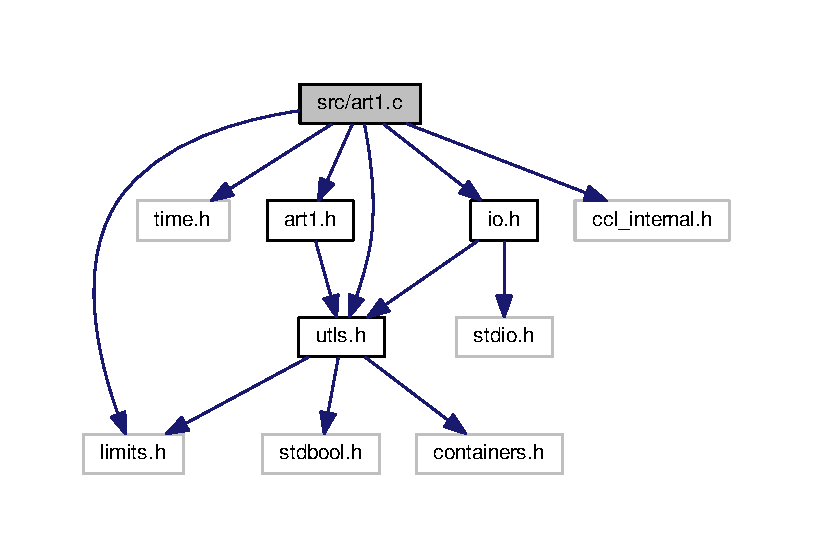
\includegraphics[width=350pt]{art1_8c__incl}
\end{center}
\end{figure}
\subsection*{Functions}
\begin{DoxyCompactItemize}
\item 
static void \hyperlink{art1_8c_aa31c8a4ded2582847654c80c3ccfcd2e}{prot\-\_\-add\-\_\-pat} (Vector $\ast$prot, Vector $\ast$pat)
\item 
static void \hyperlink{art1_8c_af42037e324f8d12d47b3816ee43870e3}{clust\-\_\-rm\-\_\-pat} (Vector $\ast$clusts, \hyperlink{utls_8h_a718b4eb2652c286f4d42dc18a8e71a1a}{ulong} i\-Clust, Vector $\ast$pats, \hyperlink{utls_8h_a718b4eb2652c286f4d42dc18a8e71a1a}{ulong} i\-Pat)
\item 
static long \hyperlink{art1_8c_adefc21b0893b11ef75642d4b6206b6cb}{com\-Ones} (Vector $\ast$pat1, Vector $\ast$pat2)
\item 
static long \hyperlink{art1_8c_a8a078c8dea015330aadc1877a0d2473a}{ones} (Vector $\ast$pat)
\item 
static void \hyperlink{art1_8c_a5217c9d063680d8924839b9f0e6bfad0}{clust\-\_\-add\-\_\-new} (Vector $\ast$clusts, Vector $\ast$pats, \hyperlink{utls_8h_a718b4eb2652c286f4d42dc18a8e71a1a}{ulong} i\-Pat)
\item 
static bool \hyperlink{art1_8c_a84b8605661376445ec3d74ec8e7d6cca}{clust\-\_\-add\-\_\-pat} (Vector $\ast$pat, Vector $\ast$pats, Vector $\ast$clusts, \hyperlink{utls_8h_a718b4eb2652c286f4d42dc18a8e71a1a}{ulong} i\-Pat, \hyperlink{utls_8h_a718b4eb2652c286f4d42dc18a8e71a1a}{ulong} i\-Candidat)
\item 
static void \hyperlink{art1_8c_adb1b5354deaf6f2e894ceb34715a36cf}{fill\-\_\-scores} (double $\ast$scores, const \hyperlink{utls_8h_a718b4eb2652c286f4d42dc18a8e71a1a}{ulong} psize, Vector $\ast$pat, Vector $\ast$clusts, float beta)
\item 
static void \hyperlink{art1_8c_a6a244d9593bbcbc30389044848bb8bea}{highest\-\_\-score} (Vector $\ast$$\ast$eq\-Scores, double $\ast$scores, \hyperlink{utls_8h_a718b4eb2652c286f4d42dc18a8e71a1a}{ulong} psize, Vector $\ast$clusts)
\item 
static \hyperlink{utls_8h_a718b4eb2652c286f4d42dc18a8e71a1a}{ulong} \hyperlink{art1_8c_a5c928b4810ec54fc333a49c26aacc624}{count\-\_\-inhib\-\_\-clusts} (Vector $\ast$clusts)
\item 
static \hyperlink{struct_cluster}{Cluster} $\ast$ \hyperlink{art1_8c_aad13cffc24501a03c4a28658a7818292}{nearest\-\_\-prot} (\hyperlink{utls_8h_a718b4eb2652c286f4d42dc18a8e71a1a}{ulong} $\ast$i\-Candidat, Vector $\ast$pat, Vector $\ast$clusts, float beta)
\item 
static void \hyperlink{art1_8c_a03b474f3089272d9f3b614dc73d8b468}{compute\-\_\-pass\-\_\-stats} (\hyperlink{utls_8h_a718b4eb2652c286f4d42dc18a8e71a1a}{ulong} $\ast$no\-Reassigned, float $\ast$fluc, Vector $\ast$reassigned, Vector $\ast$pats)
\item 
static bool \hyperlink{art1_8c_a3e69b8605f3c9eea5ef7aef29f5d5f05}{try\-\_\-next\-\_\-candidate} (\hyperlink{struct_in_param}{In\-Param} param, Vector $\ast$pats, Vector $\ast$clusts, Vector $\ast$reassigned, \hyperlink{utls_8h_a718b4eb2652c286f4d42dc18a8e71a1a}{ulong} i\-Pat)
\item 
static void \hyperlink{art1_8c_ad45139b18d1b8a8a247cb0a939b014cc}{reset\-\_\-reassigned} (Vector $\ast$reassigned)
\item 
static void \hyperlink{art1_8c_aa8367cb1a8c9a7c88c54ca019a9e6c24}{reset\-\_\-clusts\-\_\-inhib\-\_\-flags} (Vector $\ast$clusts)
\item 
void \hyperlink{art1_8c_ae84af51b551ff2e1db27eb807d0c5522}{network\-\_\-train} (Vector $\ast$$\ast$best\-Clusts, float $\ast$best\-Fluc, \hyperlink{struct_in_param}{In\-Param} par, Vector $\ast$pats)
\item 
static \hyperlink{utls_8h_a718b4eb2652c286f4d42dc18a8e71a1a}{ulong} \hyperlink{art1_8c_a1911a1940ed363f7f58050e738f076b8}{test\-\_\-next\-\_\-candidate} (\hyperlink{struct_in_param}{In\-Param} par, Vector $\ast$clusts, Vector $\ast$pats, \hyperlink{utls_8h_a718b4eb2652c286f4d42dc18a8e71a1a}{ulong} i\-Pat)
\item 
void \hyperlink{art1_8c_aac75e59787bfa49a08fa5de191779c97}{network\-\_\-test} (Vector $\ast$$\ast$test\-Res\-Classes, Vector $\ast$clusts, \hyperlink{struct_in_param}{In\-Param} par, Vector $\ast$pats, Vector $\ast$clusts\-Classes, Vector $\ast$classes)
\end{DoxyCompactItemize}


\subsection{Detailed Description}
\begin{DoxyAuthor}{Author}
Mathieu Fourcroy 
\end{DoxyAuthor}
\begin{DoxyDate}{Date}
June 2015 
\end{DoxyDate}
\begin{DoxyVersion}{Version}
0.\-0.\-1
\end{DoxyVersion}
This file contains the functions about training and testing the network.

\subsubsection*{C\-L\-U\-S\-T\-E\-R\-S }

A cluster include two things\-:
\begin{DoxyItemize}
\item A prototype\-: it's the centroid of the cluster, it's basically a pattern wich contains 1 only where every patterns of the cluster have a 1.
\item A set of patterns\-: it's the cluster members, they shape the cluster prototype.
\end{DoxyItemize}

In this programm a cluster is represented by the \hyperlink{struct_cluster}{Cluster} structure (yes, really!)

\subsubsection*{F\-L\-U\-C\-T\-U\-A\-T\-I\-O\-N }

The param.\-min\-Fluc parameter is used to indicate the maximum fluctuation percentage. The fluctuation is a function of the number of patterns which were re-\/assigned to a different cluster. The higher the number of re-\/assigned patterns, the higher the fluctuation rate. This parameter is used in order to avoid (nearly) infinite loops when training patterns.

\begin{DoxyRefDesc}{Todo}
\item[\hyperlink{todo__todo000001}{Todo}]The fluctuation rate must be increased after each pass. \end{DoxyRefDesc}


\subsection{Function Documentation}
\hypertarget{art1_8c_a5217c9d063680d8924839b9f0e6bfad0}{\index{art1.\-c@{art1.\-c}!clust\-\_\-add\-\_\-new@{clust\-\_\-add\-\_\-new}}
\index{clust\-\_\-add\-\_\-new@{clust\-\_\-add\-\_\-new}!art1.c@{art1.\-c}}
\subsubsection[{clust\-\_\-add\-\_\-new}]{\setlength{\rightskip}{0pt plus 5cm}static void clust\-\_\-add\-\_\-new (
\begin{DoxyParamCaption}
\item[{Vector $\ast$}]{clusts, }
\item[{Vector $\ast$}]{pats, }
\item[{{\bf ulong}}]{i\-Pat}
\end{DoxyParamCaption}
)\hspace{0.3cm}{\ttfamily [static]}}}\label{art1_8c_a5217c9d063680d8924839b9f0e6bfad0}
Add a new cluster to the network clusters vector.

Ceate a new cluster and initialize it by setting pattern at index 'i\-Pat' in 'pats' as its prototype and adding pattern I\-D 'i\-Pat' in its patterns set. Finaly, add the new cluster to 'clusts'.


\begin{DoxyParams}[1]{Parameters}
\mbox{\tt in,out}  & {\em clusts} & The network clusters vector where the new cluster will be added. \\
\hline
\mbox{\tt in}  & {\em pats} & The network training patterns. \\
\hline
\mbox{\tt in}  & {\em i\-Pat} & The index of the current training pattern. \\
\hline
\end{DoxyParams}


Here is the call graph for this function\-:\nopagebreak
\begin{figure}[H]
\begin{center}
\leavevmode
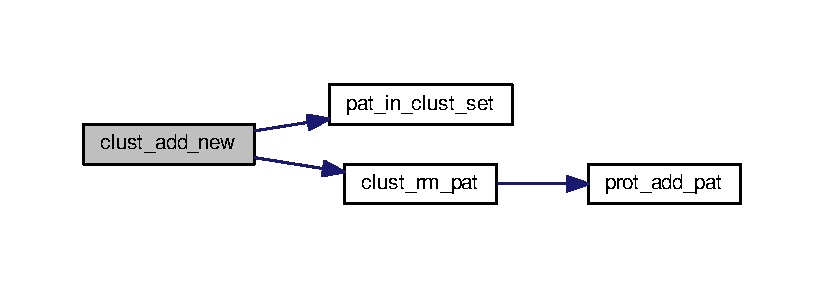
\includegraphics[width=350pt]{art1_8c_a5217c9d063680d8924839b9f0e6bfad0_cgraph}
\end{center}
\end{figure}




Here is the caller graph for this function\-:\nopagebreak
\begin{figure}[H]
\begin{center}
\leavevmode
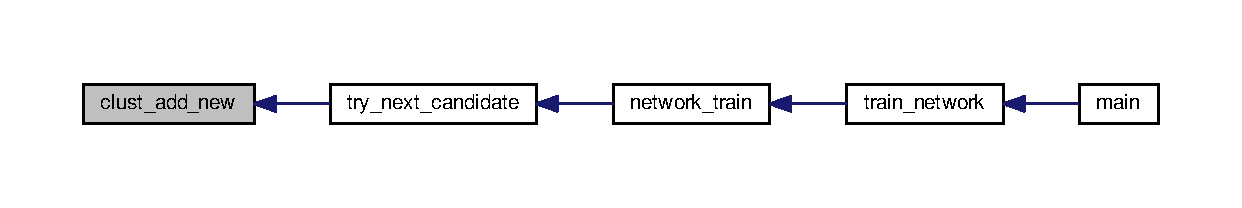
\includegraphics[width=350pt]{art1_8c_a5217c9d063680d8924839b9f0e6bfad0_icgraph}
\end{center}
\end{figure}


\hypertarget{art1_8c_a84b8605661376445ec3d74ec8e7d6cca}{\index{art1.\-c@{art1.\-c}!clust\-\_\-add\-\_\-pat@{clust\-\_\-add\-\_\-pat}}
\index{clust\-\_\-add\-\_\-pat@{clust\-\_\-add\-\_\-pat}!art1.c@{art1.\-c}}
\subsubsection[{clust\-\_\-add\-\_\-pat}]{\setlength{\rightskip}{0pt plus 5cm}static bool clust\-\_\-add\-\_\-pat (
\begin{DoxyParamCaption}
\item[{Vector $\ast$}]{pat, }
\item[{Vector $\ast$}]{pats, }
\item[{Vector $\ast$}]{clusts, }
\item[{{\bf ulong}}]{i\-Pat, }
\item[{{\bf ulong}}]{i\-Candidat}
\end{DoxyParamCaption}
)\hspace{0.3cm}{\ttfamily [static]}}}\label{art1_8c_a84b8605661376445ec3d74ec8e7d6cca}
Add a pattern to a cluster.

To add a pattern to a candidate cluster we must\-:
\begin{DoxyItemize}
\item Add the pattern I\-D to the cluster patterns set
\item Reshape the cluster prototype.
\end{DoxyItemize}

If the pattern already belongs to another cluster then it is removed from this cluster and added to the candidate cluster (reassignement) and true is returned. If the pattern already belongs to the candidate cluster then false is returned and the algorithm should go with the next pattern to train. Else, if the pattern dosen't already belongs to any cluster then it is simply added to the candidate cluster and true is returned.


\begin{DoxyParams}[1]{Parameters}
\mbox{\tt in}  & {\em pat} & The pattern to add to the cluster. \\
\hline
\mbox{\tt in}  & {\em pats} & The network training patterns set. \\
\hline
\mbox{\tt in,out}  & {\em clusts} & The network clusters. \\
\hline
\mbox{\tt in}  & {\em i\-Pat} & The index of 'pat' in 'pats'. \\
\hline
\mbox{\tt in}  & {\em i\-Candidate} & The index of the cluter in which the pattern will be added.\\
\hline
\end{DoxyParams}
\begin{DoxyReturn}{Returns}
true if the pattern has been added to the cluster ; false if the pattern already belongs to the cluster. 
\end{DoxyReturn}


Here is the call graph for this function\-:\nopagebreak
\begin{figure}[H]
\begin{center}
\leavevmode
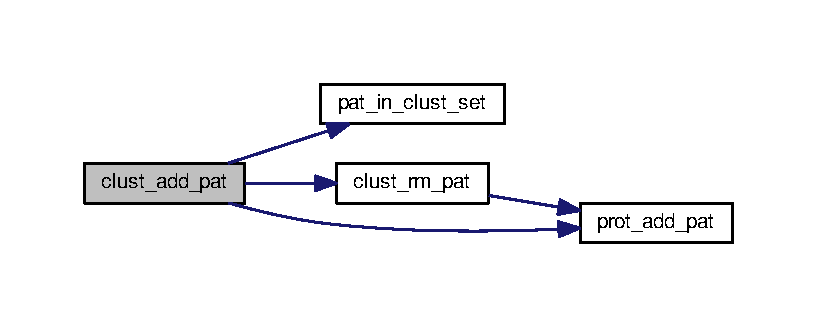
\includegraphics[width=350pt]{art1_8c_a84b8605661376445ec3d74ec8e7d6cca_cgraph}
\end{center}
\end{figure}




Here is the caller graph for this function\-:\nopagebreak
\begin{figure}[H]
\begin{center}
\leavevmode
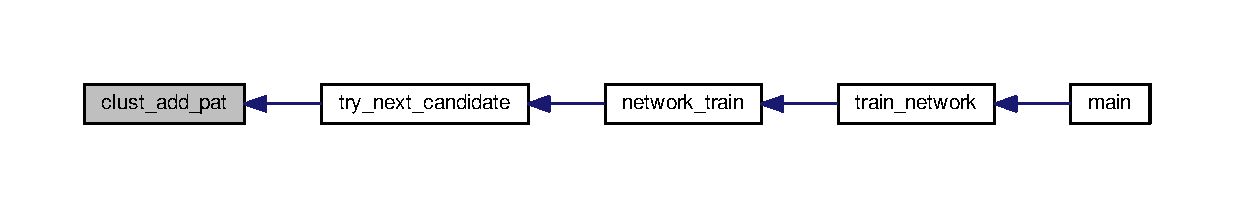
\includegraphics[width=350pt]{art1_8c_a84b8605661376445ec3d74ec8e7d6cca_icgraph}
\end{center}
\end{figure}


\hypertarget{art1_8c_af42037e324f8d12d47b3816ee43870e3}{\index{art1.\-c@{art1.\-c}!clust\-\_\-rm\-\_\-pat@{clust\-\_\-rm\-\_\-pat}}
\index{clust\-\_\-rm\-\_\-pat@{clust\-\_\-rm\-\_\-pat}!art1.c@{art1.\-c}}
\subsubsection[{clust\-\_\-rm\-\_\-pat}]{\setlength{\rightskip}{0pt plus 5cm}static void clust\-\_\-rm\-\_\-pat (
\begin{DoxyParamCaption}
\item[{Vector $\ast$}]{clusts, }
\item[{{\bf ulong}}]{i\-Clust, }
\item[{Vector $\ast$}]{pats, }
\item[{{\bf ulong}}]{i\-Pat}
\end{DoxyParamCaption}
)\hspace{0.3cm}{\ttfamily [static]}}}\label{art1_8c_af42037e324f8d12d47b3816ee43870e3}
Remove the given pattern from the given cluster.

Remove the pattern at index 'i\-Pat' of 'pats' from cluster prototype at index 'i\-Clust' of 'clusts'. Also remove the pattern I\-D from the prototype patterns set.


\begin{DoxyParams}[1]{Parameters}
\mbox{\tt in}  & {\em pats} & The network training patterns set. \\
\hline
\mbox{\tt in}  & {\em i\-Pat} & The index of the pattern to remove. \\
\hline
\mbox{\tt in,out}  & {\em clusts} & The network clusters. \\
\hline
\mbox{\tt in}  & {\em i\-Clust} & The index of the cluster from which the pattern will be removed. \\
\hline
\end{DoxyParams}


Here is the call graph for this function\-:\nopagebreak
\begin{figure}[H]
\begin{center}
\leavevmode
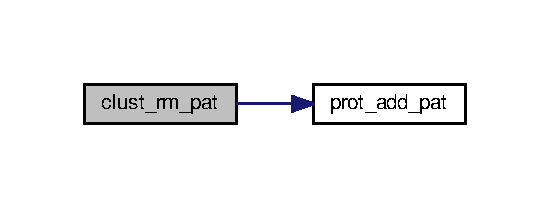
\includegraphics[width=264pt]{art1_8c_af42037e324f8d12d47b3816ee43870e3_cgraph}
\end{center}
\end{figure}




Here is the caller graph for this function\-:\nopagebreak
\begin{figure}[H]
\begin{center}
\leavevmode
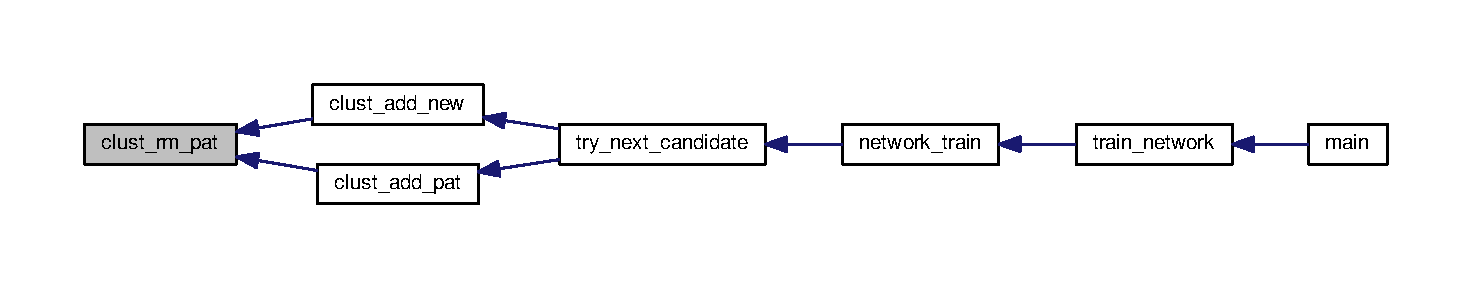
\includegraphics[width=350pt]{art1_8c_af42037e324f8d12d47b3816ee43870e3_icgraph}
\end{center}
\end{figure}


\hypertarget{art1_8c_adefc21b0893b11ef75642d4b6206b6cb}{\index{art1.\-c@{art1.\-c}!com\-Ones@{com\-Ones}}
\index{com\-Ones@{com\-Ones}!art1.c@{art1.\-c}}
\subsubsection[{com\-Ones}]{\setlength{\rightskip}{0pt plus 5cm}static long com\-Ones (
\begin{DoxyParamCaption}
\item[{Vector $\ast$}]{pat1, }
\item[{Vector $\ast$}]{pat2}
\end{DoxyParamCaption}
)\hspace{0.3cm}{\ttfamily [static]}}}\label{art1_8c_adefc21b0893b11ef75642d4b6206b6cb}
Returns the number of 1 that the two given patterns have in common.

Count and return the number of 1 which are present in 'pat1' and 'pat2', at same indexes.

\begin{DoxyNote}{Note}
'pat1' and 'pat2' must have the same length. It is admit and it's obvious because the program check it at the begining so no test are carried out here in order to save time.
\end{DoxyNote}

\begin{DoxyParams}[1]{Parameters}
\mbox{\tt in}  & {\em pat1} & The first pattern, will be compared to 'pat2'. \\
\hline
\mbox{\tt in}  & {\em pat2} & The second pattern, will be compared to 'pat1'.\\
\hline
\end{DoxyParams}
\begin{DoxyReturn}{Returns}
The number of 1 that the two given patterns have in common. 
\end{DoxyReturn}


Here is the caller graph for this function\-:\nopagebreak
\begin{figure}[H]
\begin{center}
\leavevmode
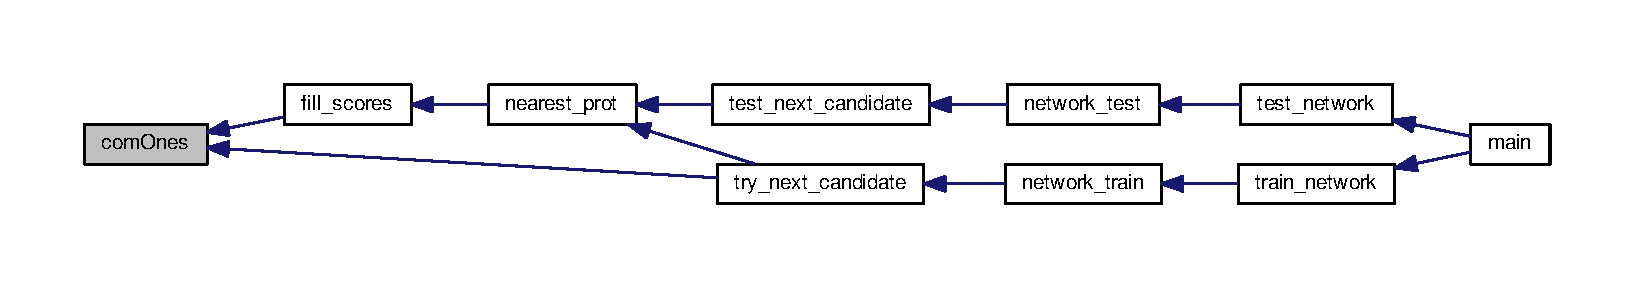
\includegraphics[width=350pt]{art1_8c_adefc21b0893b11ef75642d4b6206b6cb_icgraph}
\end{center}
\end{figure}


\hypertarget{art1_8c_a03b474f3089272d9f3b614dc73d8b468}{\index{art1.\-c@{art1.\-c}!compute\-\_\-pass\-\_\-stats@{compute\-\_\-pass\-\_\-stats}}
\index{compute\-\_\-pass\-\_\-stats@{compute\-\_\-pass\-\_\-stats}!art1.c@{art1.\-c}}
\subsubsection[{compute\-\_\-pass\-\_\-stats}]{\setlength{\rightskip}{0pt plus 5cm}static void compute\-\_\-pass\-\_\-stats (
\begin{DoxyParamCaption}
\item[{{\bf ulong} $\ast$}]{no\-Reassigned, }
\item[{float $\ast$}]{fluc, }
\item[{Vector $\ast$}]{reassigned, }
\item[{Vector $\ast$}]{pats}
\end{DoxyParamCaption}
)\hspace{0.3cm}{\ttfamily [static]}}}\label{art1_8c_a03b474f3089272d9f3b614dc73d8b468}
Compute the statistics of the last training pass.

Sets the 'no\-Reassigned' parameter (number of patterns reassigned to another cluster during the pass) and the 'fluc' parameter (fluctuation percentage for the pass).


\begin{DoxyParams}[1]{Parameters}
\mbox{\tt out}  & {\em no\-Reassigned} & Number of patterns which have been assigned to another cluster during the pass. \\
\hline
\mbox{\tt out}  & {\em fluc} & Fluctuation percentage of the pass. \\
\hline
\mbox{\tt in}  & {\em reassigned} & Array of values indicating the I\-D of the patterns which have been reassigned to another cluster (I\-D is the index in the array). \\
\hline
\mbox{\tt in}  & {\em pats} & The network training patterns set. \\
\hline
\end{DoxyParams}


Here is the caller graph for this function\-:\nopagebreak
\begin{figure}[H]
\begin{center}
\leavevmode
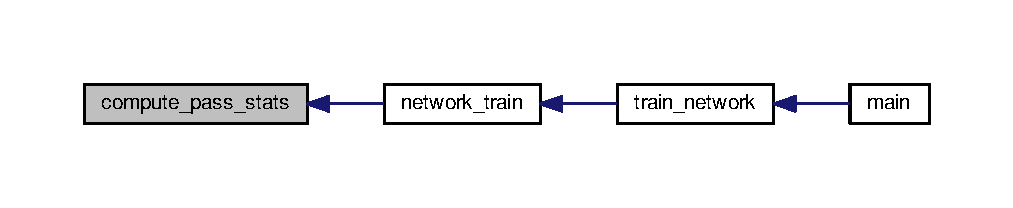
\includegraphics[width=350pt]{art1_8c_a03b474f3089272d9f3b614dc73d8b468_icgraph}
\end{center}
\end{figure}


\hypertarget{art1_8c_a5c928b4810ec54fc333a49c26aacc624}{\index{art1.\-c@{art1.\-c}!count\-\_\-inhib\-\_\-clusts@{count\-\_\-inhib\-\_\-clusts}}
\index{count\-\_\-inhib\-\_\-clusts@{count\-\_\-inhib\-\_\-clusts}!art1.c@{art1.\-c}}
\subsubsection[{count\-\_\-inhib\-\_\-clusts}]{\setlength{\rightskip}{0pt plus 5cm}static {\bf ulong} count\-\_\-inhib\-\_\-clusts (
\begin{DoxyParamCaption}
\item[{Vector $\ast$}]{clusts}
\end{DoxyParamCaption}
)\hspace{0.3cm}{\ttfamily [static]}}}\label{art1_8c_a5c928b4810ec54fc333a49c26aacc624}
Returns the number of inhibited clusters.


\begin{DoxyParams}[1]{Parameters}
\mbox{\tt in}  & {\em clusts} & The network clusters.\\
\hline
\end{DoxyParams}
\begin{DoxyReturn}{Returns}
The number of inhibited clusters. 
\end{DoxyReturn}


Here is the caller graph for this function\-:\nopagebreak
\begin{figure}[H]
\begin{center}
\leavevmode
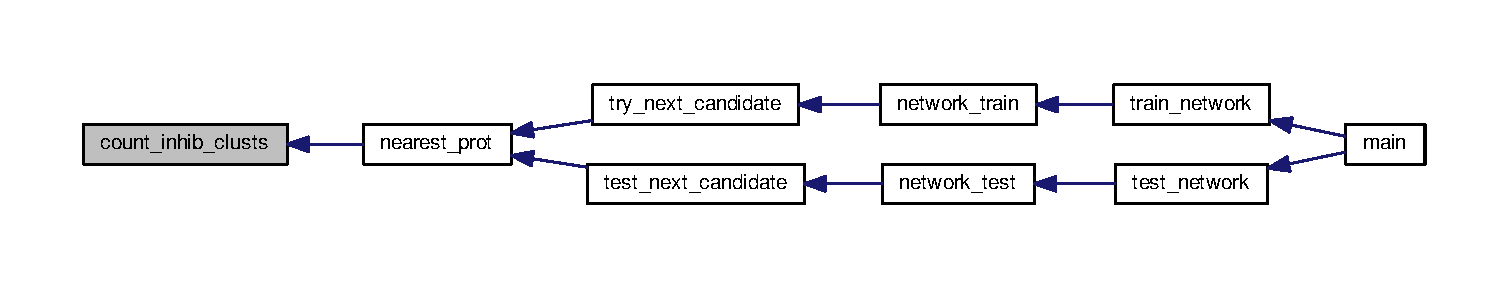
\includegraphics[width=350pt]{art1_8c_a5c928b4810ec54fc333a49c26aacc624_icgraph}
\end{center}
\end{figure}


\hypertarget{art1_8c_adb1b5354deaf6f2e894ceb34715a36cf}{\index{art1.\-c@{art1.\-c}!fill\-\_\-scores@{fill\-\_\-scores}}
\index{fill\-\_\-scores@{fill\-\_\-scores}!art1.c@{art1.\-c}}
\subsubsection[{fill\-\_\-scores}]{\setlength{\rightskip}{0pt plus 5cm}static void fill\-\_\-scores (
\begin{DoxyParamCaption}
\item[{double $\ast$}]{scores, }
\item[{const {\bf ulong}}]{psize, }
\item[{Vector $\ast$}]{pat, }
\item[{Vector $\ast$}]{clusts, }
\item[{float}]{beta}
\end{DoxyParamCaption}
)\hspace{0.3cm}{\ttfamily [static]}}}\label{art1_8c_adb1b5354deaf6f2e894ceb34715a36cf}
Fill the score array with the computed scores of the network prototypes.

Fill the 'score' array with a score value for each cluster prototype in 'clusts'. The score value represents the similarity level between the actual pattern and a cluster prototype. If a prototype is inhibited then its score is N\-O\-N\-E.

\begin{DoxyNote}{Note}
The calculation is based on the 'beta' parameter, the pattern 'pat' and the cluster prototypes.

The 'clusts' vector size, is passed as parameter 'psize' in order to avoid a second \hyperlink{utls_8h_a12bdf08e246ee2dbf37483c33b5c28df}{vec\-\_\-size()} call.
\end{DoxyNote}

\begin{DoxyParams}[1]{Parameters}
\mbox{\tt out}  & {\em scores} & The scores array to fill. \\
\hline
\mbox{\tt in}  & {\em psize} & Number of clusters of the network. \\
\hline
\mbox{\tt in}  & {\em pat} & The current training pattern. \\
\hline
\mbox{\tt in}  & {\em clusts} & The network cllusters. \\
\hline
\mbox{\tt in}  & {\em beta} & The network beta parameter. \\
\hline
\end{DoxyParams}


Here is the call graph for this function\-:\nopagebreak
\begin{figure}[H]
\begin{center}
\leavevmode
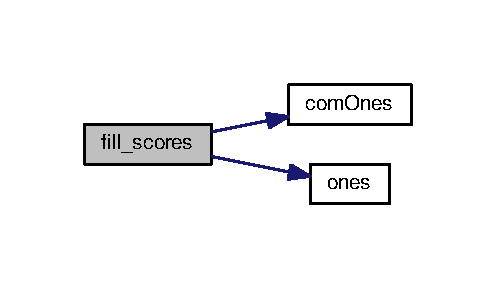
\includegraphics[width=238pt]{art1_8c_adb1b5354deaf6f2e894ceb34715a36cf_cgraph}
\end{center}
\end{figure}




Here is the caller graph for this function\-:\nopagebreak
\begin{figure}[H]
\begin{center}
\leavevmode
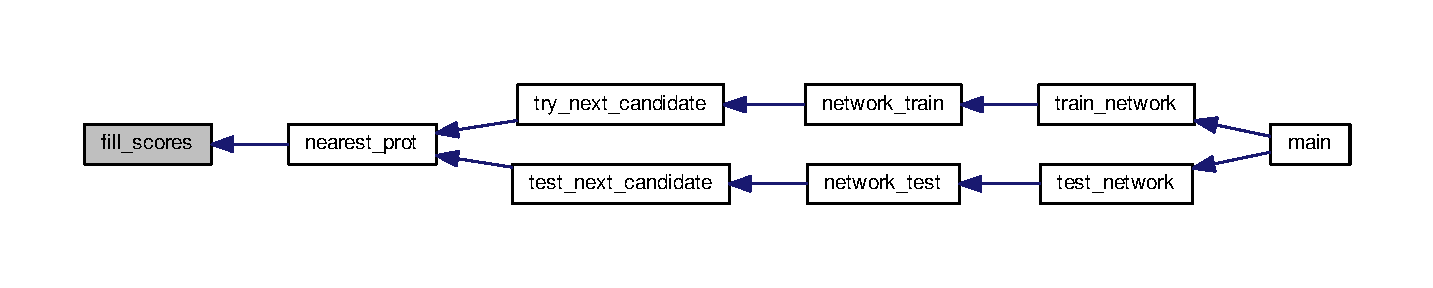
\includegraphics[width=350pt]{art1_8c_adb1b5354deaf6f2e894ceb34715a36cf_icgraph}
\end{center}
\end{figure}


\hypertarget{art1_8c_a6a244d9593bbcbc30389044848bb8bea}{\index{art1.\-c@{art1.\-c}!highest\-\_\-score@{highest\-\_\-score}}
\index{highest\-\_\-score@{highest\-\_\-score}!art1.c@{art1.\-c}}
\subsubsection[{highest\-\_\-score}]{\setlength{\rightskip}{0pt plus 5cm}static void highest\-\_\-score (
\begin{DoxyParamCaption}
\item[{Vector $\ast$$\ast$}]{eq\-Scores, }
\item[{double $\ast$}]{scores, }
\item[{{\bf ulong}}]{psize, }
\item[{Vector $\ast$}]{clusts}
\end{DoxyParamCaption}
)\hspace{0.3cm}{\ttfamily [static]}}}\label{art1_8c_a6a244d9593bbcbc30389044848bb8bea}
Compute the highest score in the 'scores' array.

The 'eq\-Scores' array is modified to contain the highest score prototype(s) I\-D(s) (there can be multiple prototypes with the same highest score that's why 'eq\-Scores' is a vector).


\begin{DoxyParams}[1]{Parameters}
\mbox{\tt out}  & {\em eq\-Scores} & The scores array to fill with every highest scores. \\
\hline
\mbox{\tt in}  & {\em scores} & The array containing the prototypes's scores. \\
\hline
\mbox{\tt in}  & {\em psize} & Number of clusters of the network. \\
\hline
\mbox{\tt in}  & {\em clusts} & The network cllusters. \\
\hline
\end{DoxyParams}


Here is the caller graph for this function\-:\nopagebreak
\begin{figure}[H]
\begin{center}
\leavevmode
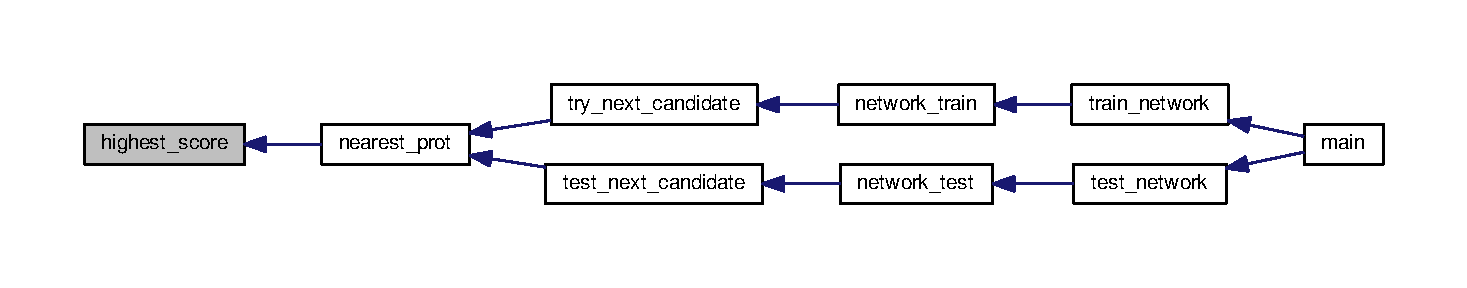
\includegraphics[width=350pt]{art1_8c_a6a244d9593bbcbc30389044848bb8bea_icgraph}
\end{center}
\end{figure}


\hypertarget{art1_8c_aad13cffc24501a03c4a28658a7818292}{\index{art1.\-c@{art1.\-c}!nearest\-\_\-prot@{nearest\-\_\-prot}}
\index{nearest\-\_\-prot@{nearest\-\_\-prot}!art1.c@{art1.\-c}}
\subsubsection[{nearest\-\_\-prot}]{\setlength{\rightskip}{0pt plus 5cm}static {\bf Cluster}$\ast$ nearest\-\_\-prot (
\begin{DoxyParamCaption}
\item[{{\bf ulong} $\ast$}]{i\-Candidat, }
\item[{Vector $\ast$}]{pat, }
\item[{Vector $\ast$}]{clusts, }
\item[{float}]{beta}
\end{DoxyParamCaption}
)\hspace{0.3cm}{\ttfamily [static]}}}\label{art1_8c_aad13cffc24501a03c4a28658a7818292}
Compute and returns the uninhibited prototype closest to a given pattern.

To achieve this, the function first compute the \char`\"{}similarity score\char`\"{} of every uninhibited prototypes (inhibited prototypes have a score of -\/1) then it computes the prototype with the highest score (if more than one prototype with equal highest score then the returned one is randomly chosen). If all clusters are inhibited then the function return false.

\begin{DoxyNote}{Note}
It would be more C-\/style to return a bool indicating if a candidate has been found or not and set it via a passed argument. But this way it is easier for freeing.
\end{DoxyNote}

\begin{DoxyParams}[1]{Parameters}
\mbox{\tt out}  & {\em candidat} & The uninhibited prototype closest to a given pattern (the candidate). \\
\hline
\mbox{\tt out}  & {\em i\-Candidat} & The index of the computed candidate. \\
\hline
\mbox{\tt in}  & {\em pat} & The reference pattern. \\
\hline
\mbox{\tt in}  & {\em clusts} & The network clusters. \\
\hline
\mbox{\tt in}  & {\em beta} & The network beta parameter.\\
\hline
\end{DoxyParams}
\begin{DoxyReturn}{Returns}
true or false weither a candidate has been found. 
\end{DoxyReturn}


Here is the call graph for this function\-:\nopagebreak
\begin{figure}[H]
\begin{center}
\leavevmode
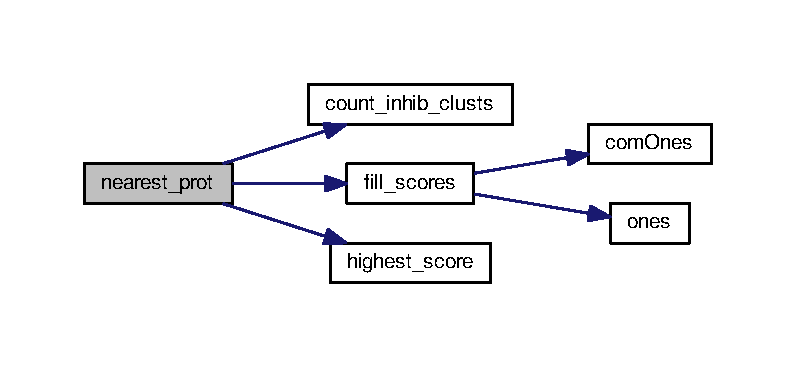
\includegraphics[width=350pt]{art1_8c_aad13cffc24501a03c4a28658a7818292_cgraph}
\end{center}
\end{figure}




Here is the caller graph for this function\-:\nopagebreak
\begin{figure}[H]
\begin{center}
\leavevmode
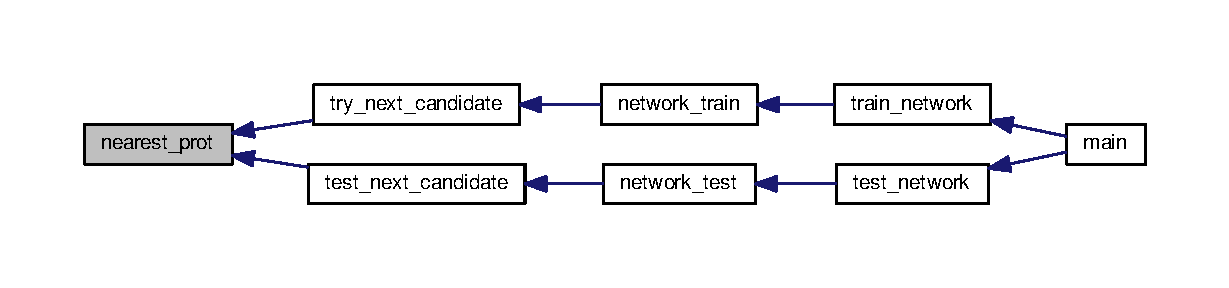
\includegraphics[width=350pt]{art1_8c_aad13cffc24501a03c4a28658a7818292_icgraph}
\end{center}
\end{figure}


\hypertarget{art1_8c_aac75e59787bfa49a08fa5de191779c97}{\index{art1.\-c@{art1.\-c}!network\-\_\-test@{network\-\_\-test}}
\index{network\-\_\-test@{network\-\_\-test}!art1.c@{art1.\-c}}
\subsubsection[{network\-\_\-test}]{\setlength{\rightskip}{0pt plus 5cm}void network\-\_\-test (
\begin{DoxyParamCaption}
\item[{Vector $\ast$$\ast$}]{test\-Res\-Classes, }
\item[{Vector $\ast$}]{clusts, }
\item[{{\bf In\-Param}}]{par, }
\item[{Vector $\ast$}]{pats, }
\item[{Vector $\ast$}]{clusts\-Classes, }
\item[{Vector $\ast$}]{classes}
\end{DoxyParamCaption}
)}}\label{art1_8c_aac75e59787bfa49a08fa5de191779c97}


Here is the call graph for this function\-:\nopagebreak
\begin{figure}[H]
\begin{center}
\leavevmode
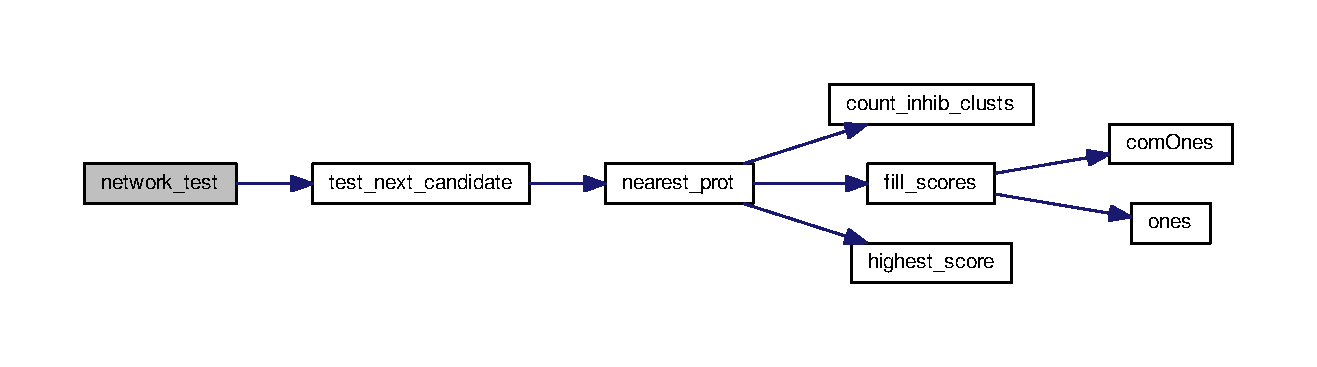
\includegraphics[width=350pt]{art1_8c_aac75e59787bfa49a08fa5de191779c97_cgraph}
\end{center}
\end{figure}




Here is the caller graph for this function\-:\nopagebreak
\begin{figure}[H]
\begin{center}
\leavevmode
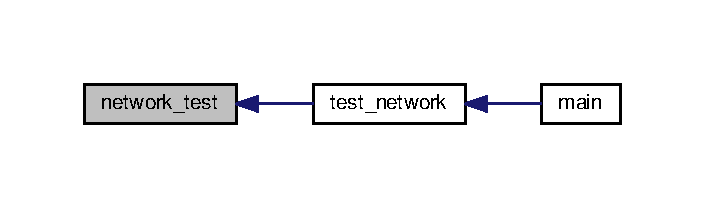
\includegraphics[width=338pt]{art1_8c_aac75e59787bfa49a08fa5de191779c97_icgraph}
\end{center}
\end{figure}


\hypertarget{art1_8c_ae84af51b551ff2e1db27eb807d0c5522}{\index{art1.\-c@{art1.\-c}!network\-\_\-train@{network\-\_\-train}}
\index{network\-\_\-train@{network\-\_\-train}!art1.c@{art1.\-c}}
\subsubsection[{network\-\_\-train}]{\setlength{\rightskip}{0pt plus 5cm}void network\-\_\-train (
\begin{DoxyParamCaption}
\item[{Vector $\ast$$\ast$}]{best\-Clusts, }
\item[{float $\ast$}]{best\-Fluc, }
\item[{{\bf In\-Param}}]{par, }
\item[{Vector $\ast$}]{pats}
\end{DoxyParamCaption}
)}}\label{art1_8c_ae84af51b551ff2e1db27eb807d0c5522}
Train the network using the training patterns set and the parameters.

It loops until at least one stop condition is met. There's two stop conditions\-:
\begin{DoxyItemize}
\item Stop when the number of performed passes reaches the maximum number of passes (par-\/$>$max\-Passes).
\item Stop when the fluctuation rate is lower than or equal to the maximum fluctuation percentage (par-\/$>$min\-Fluc).
\end{DoxyItemize}

Inside this while loop there's a for loop which loops for each training patterns. And inside this for loop there's a second while loop which loops until the pattern is successfuly added to an existing or a new cluster.

The function looks like\-:\-:

L\-O\-O\-P W\-H\-I\-L\-E ( pass $<$ max\-Passes ) A\-N\-D ( fluc $>$ min\-Fluc )\-: L\-O\-O\-P F\-O\-R pat I\-N pats\-: D\-O\-: candidat = pick\-\_\-a\-\_\-candidat(clusters, pat) W\-H\-I\-L\-E N\-O\-T fits\-\_\-in\-\_\-candidat(candidat, pat)


\begin{DoxyParams}[1]{Parameters}
\mbox{\tt out}  & {\em best\-Clusts} & \\
\hline
\mbox{\tt out}  & {\em best\-Fluc} & \\
\hline
\mbox{\tt in}  & {\em pats} & \\
\hline
\mbox{\tt in}  & {\em par} & \\
\hline
\end{DoxyParams}


Here is the call graph for this function\-:\nopagebreak
\begin{figure}[H]
\begin{center}
\leavevmode
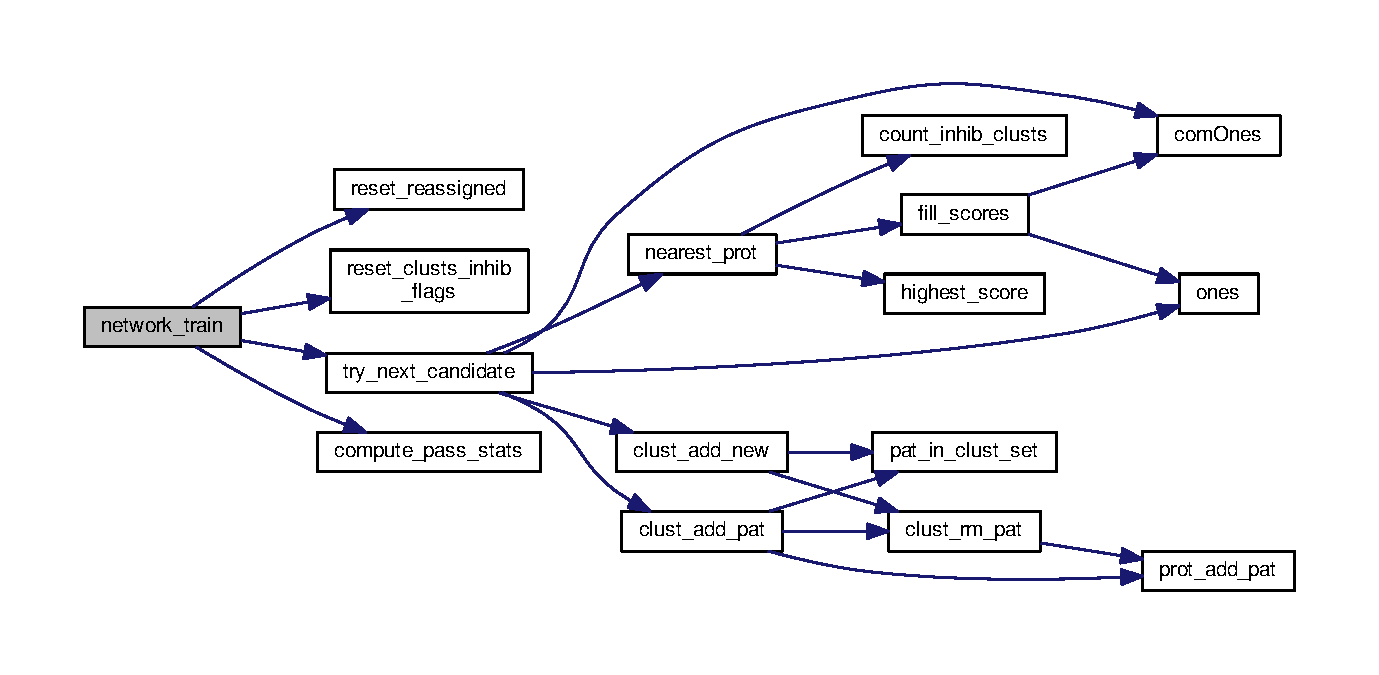
\includegraphics[width=350pt]{art1_8c_ae84af51b551ff2e1db27eb807d0c5522_cgraph}
\end{center}
\end{figure}




Here is the caller graph for this function\-:\nopagebreak
\begin{figure}[H]
\begin{center}
\leavevmode
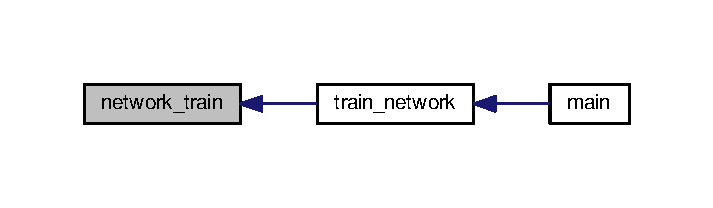
\includegraphics[width=342pt]{art1_8c_ae84af51b551ff2e1db27eb807d0c5522_icgraph}
\end{center}
\end{figure}


\hypertarget{art1_8c_a8a078c8dea015330aadc1877a0d2473a}{\index{art1.\-c@{art1.\-c}!ones@{ones}}
\index{ones@{ones}!art1.c@{art1.\-c}}
\subsubsection[{ones}]{\setlength{\rightskip}{0pt plus 5cm}static long ones (
\begin{DoxyParamCaption}
\item[{Vector $\ast$}]{pat}
\end{DoxyParamCaption}
)\hspace{0.3cm}{\ttfamily [static]}}}\label{art1_8c_a8a078c8dea015330aadc1877a0d2473a}
Returns number of 1 in a given pattern (or a prototype).


\begin{DoxyParams}[1]{Parameters}
\mbox{\tt in}  & {\em pat} & The pattern.\\
\hline
\end{DoxyParams}
\begin{DoxyReturn}{Returns}
The number of 1 in the given pattern. 
\end{DoxyReturn}


Here is the caller graph for this function\-:\nopagebreak
\begin{figure}[H]
\begin{center}
\leavevmode
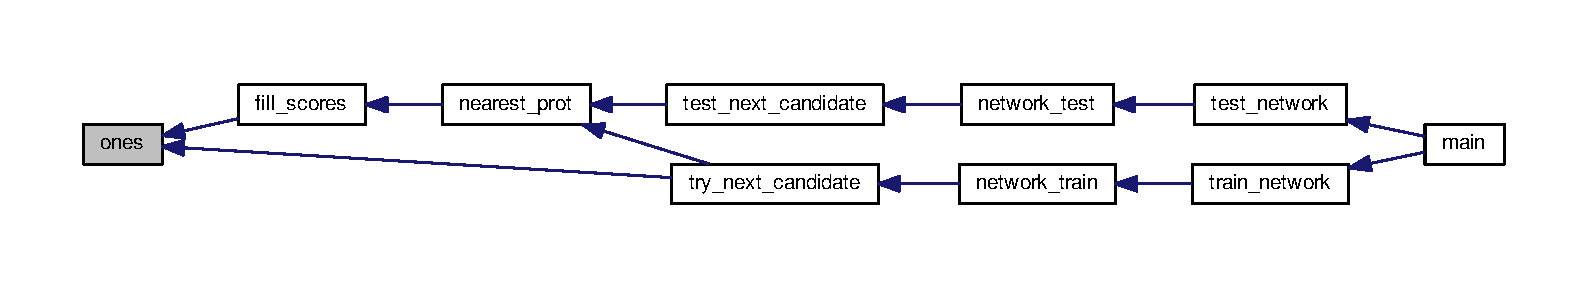
\includegraphics[width=350pt]{art1_8c_a8a078c8dea015330aadc1877a0d2473a_icgraph}
\end{center}
\end{figure}


\hypertarget{art1_8c_aa31c8a4ded2582847654c80c3ccfcd2e}{\index{art1.\-c@{art1.\-c}!prot\-\_\-add\-\_\-pat@{prot\-\_\-add\-\_\-pat}}
\index{prot\-\_\-add\-\_\-pat@{prot\-\_\-add\-\_\-pat}!art1.c@{art1.\-c}}
\subsubsection[{prot\-\_\-add\-\_\-pat}]{\setlength{\rightskip}{0pt plus 5cm}static void prot\-\_\-add\-\_\-pat (
\begin{DoxyParamCaption}
\item[{Vector $\ast$}]{prot, }
\item[{Vector $\ast$}]{pat}
\end{DoxyParamCaption}
)\hspace{0.3cm}{\ttfamily [static]}}}\label{art1_8c_aa31c8a4ded2582847654c80c3ccfcd2e}
Add a given pattern to a cluster prototype.

Add pattern 'pat' to a cluster prototype 'prot'. The prototype 'prot' will be more similar to this pattern because if it has a 1 where pattern have a 0 then the 1 become a 0.

\begin{DoxyNote}{Note}
A prototype have a 1 only where every member patterns have a 1.
\end{DoxyNote}

\begin{DoxyParams}[1]{Parameters}
\mbox{\tt in,out}  & {\em prot} & The prototype that will be modified to ressembles the pattern. \\
\hline
\mbox{\tt in}  & {\em pat} & The pattern to add to the prototype. \\
\hline
\end{DoxyParams}


Here is the caller graph for this function\-:\nopagebreak
\begin{figure}[H]
\begin{center}
\leavevmode
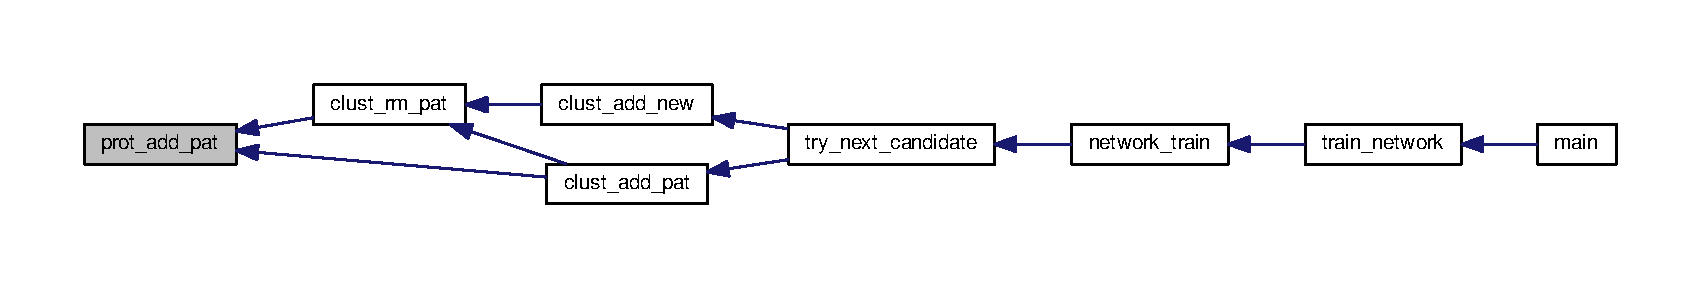
\includegraphics[width=350pt]{art1_8c_aa31c8a4ded2582847654c80c3ccfcd2e_icgraph}
\end{center}
\end{figure}


\hypertarget{art1_8c_aa8367cb1a8c9a7c88c54ca019a9e6c24}{\index{art1.\-c@{art1.\-c}!reset\-\_\-clusts\-\_\-inhib\-\_\-flags@{reset\-\_\-clusts\-\_\-inhib\-\_\-flags}}
\index{reset\-\_\-clusts\-\_\-inhib\-\_\-flags@{reset\-\_\-clusts\-\_\-inhib\-\_\-flags}!art1.c@{art1.\-c}}
\subsubsection[{reset\-\_\-clusts\-\_\-inhib\-\_\-flags}]{\setlength{\rightskip}{0pt plus 5cm}static void reset\-\_\-clusts\-\_\-inhib\-\_\-flags (
\begin{DoxyParamCaption}
\item[{Vector $\ast$}]{clusts}
\end{DoxyParamCaption}
)\hspace{0.3cm}{\ttfamily [static]}}}\label{art1_8c_aa8367cb1a8c9a7c88c54ca019a9e6c24}
Set the inhib flag of every elements of the vector to false.

The clusts vector containg the clusters of the network. Each cluster has an \char`\"{}inhib\char`\"{} flag which indicate if it has been inhibited or not. Before trying to add a pattern in a cluster, every clusters inhib flag must be set back to false.


\begin{DoxyParams}[1]{Parameters}
\mbox{\tt in,out}  & {\em clusts} & The vector containing the clusters. \\
\hline
\end{DoxyParams}


Here is the caller graph for this function\-:\nopagebreak
\begin{figure}[H]
\begin{center}
\leavevmode
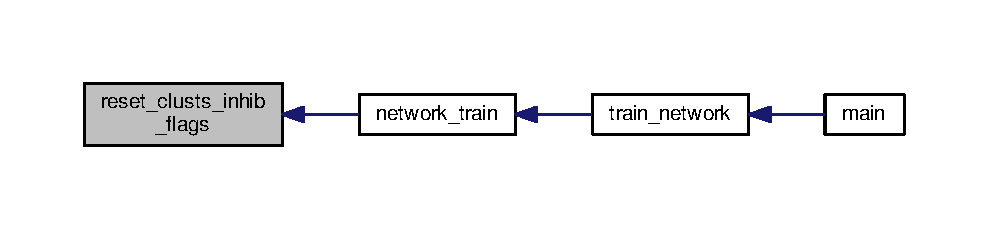
\includegraphics[width=350pt]{art1_8c_aa8367cb1a8c9a7c88c54ca019a9e6c24_icgraph}
\end{center}
\end{figure}


\hypertarget{art1_8c_ad45139b18d1b8a8a247cb0a939b014cc}{\index{art1.\-c@{art1.\-c}!reset\-\_\-reassigned@{reset\-\_\-reassigned}}
\index{reset\-\_\-reassigned@{reset\-\_\-reassigned}!art1.c@{art1.\-c}}
\subsubsection[{reset\-\_\-reassigned}]{\setlength{\rightskip}{0pt plus 5cm}static void reset\-\_\-reassigned (
\begin{DoxyParamCaption}
\item[{Vector $\ast$}]{reassigned}
\end{DoxyParamCaption}
)\hspace{0.3cm}{\ttfamily [static]}}}\label{art1_8c_ad45139b18d1b8a8a247cb0a939b014cc}
Set every elements of the vector to false.

The reassigned vector contains one flag for each pattern of the training patterns set which indicate if the pattern has been reassigned or not. At the begining of every passes these flags must be set back to false.


\begin{DoxyParams}[1]{Parameters}
\mbox{\tt in,out}  & {\em reassigned} & The vector containing the flags to reset. \\
\hline
\end{DoxyParams}


Here is the caller graph for this function\-:\nopagebreak
\begin{figure}[H]
\begin{center}
\leavevmode
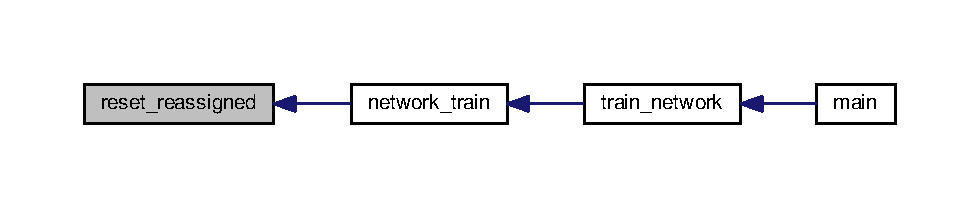
\includegraphics[width=350pt]{art1_8c_ad45139b18d1b8a8a247cb0a939b014cc_icgraph}
\end{center}
\end{figure}


\hypertarget{art1_8c_a1911a1940ed363f7f58050e738f076b8}{\index{art1.\-c@{art1.\-c}!test\-\_\-next\-\_\-candidate@{test\-\_\-next\-\_\-candidate}}
\index{test\-\_\-next\-\_\-candidate@{test\-\_\-next\-\_\-candidate}!art1.c@{art1.\-c}}
\subsubsection[{test\-\_\-next\-\_\-candidate}]{\setlength{\rightskip}{0pt plus 5cm}static {\bf ulong} test\-\_\-next\-\_\-candidate (
\begin{DoxyParamCaption}
\item[{{\bf In\-Param}}]{par, }
\item[{Vector $\ast$}]{clusts, }
\item[{Vector $\ast$}]{pats, }
\item[{{\bf ulong}}]{i\-Pat}
\end{DoxyParamCaption}
)\hspace{0.3cm}{\ttfamily [static]}}}\label{art1_8c_a1911a1940ed363f7f58050e738f076b8}


Here is the call graph for this function\-:\nopagebreak
\begin{figure}[H]
\begin{center}
\leavevmode
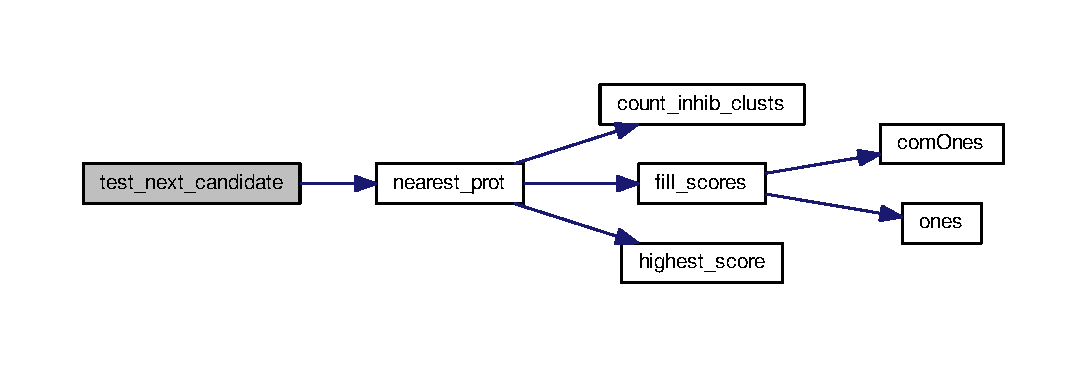
\includegraphics[width=350pt]{art1_8c_a1911a1940ed363f7f58050e738f076b8_cgraph}
\end{center}
\end{figure}




Here is the caller graph for this function\-:\nopagebreak
\begin{figure}[H]
\begin{center}
\leavevmode
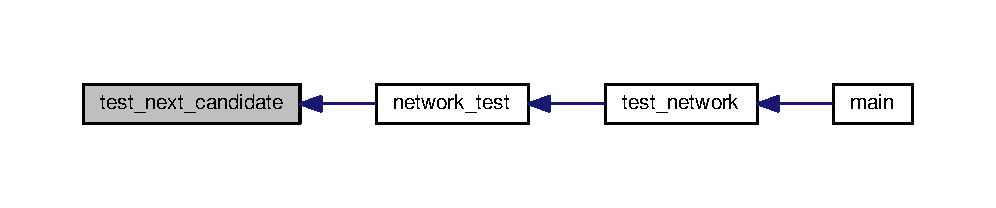
\includegraphics[width=350pt]{art1_8c_a1911a1940ed363f7f58050e738f076b8_icgraph}
\end{center}
\end{figure}


\hypertarget{art1_8c_a3e69b8605f3c9eea5ef7aef29f5d5f05}{\index{art1.\-c@{art1.\-c}!try\-\_\-next\-\_\-candidate@{try\-\_\-next\-\_\-candidate}}
\index{try\-\_\-next\-\_\-candidate@{try\-\_\-next\-\_\-candidate}!art1.c@{art1.\-c}}
\subsubsection[{try\-\_\-next\-\_\-candidate}]{\setlength{\rightskip}{0pt plus 5cm}static bool try\-\_\-next\-\_\-candidate (
\begin{DoxyParamCaption}
\item[{{\bf In\-Param}}]{param, }
\item[{Vector $\ast$}]{pats, }
\item[{Vector $\ast$}]{clusts, }
\item[{Vector $\ast$}]{reassigned, }
\item[{{\bf ulong}}]{i\-Pat}
\end{DoxyParamCaption}
)\hspace{0.3cm}{\ttfamily [static]}}}\label{art1_8c_a3e69b8605f3c9eea5ef7aef29f5d5f05}
Select a cluster candidate and try to add the pattern to this candidate.

Select the nearest prototype of the pattern at index 'i\-Pat' in 'pats' (the candidate) and check if the pattern can fits in the candidate's cluster depending on beta and vigilance parameters. If the pattern fits in the cluster, then it is added to it, else, a new cluster is create and the pattern became its prototype.


\begin{DoxyParams}[1]{Parameters}
\mbox{\tt in}  & {\em param} & The network parameters. \\
\hline
\mbox{\tt in}  & {\em pats} & The training patterns set. \\
\hline
\mbox{\tt in,out}  & {\em clusts} & The network clusters. \\
\hline
\mbox{\tt in,out}  & {\em reassigned} & The reassigned pattern flags. \\
\hline
\mbox{\tt in}  & {\em i\-Pat} & The index of the current training pattern to assigned to a cluster.\\
\hline
\end{DoxyParams}
\begin{DoxyReturn}{Returns}
true or false weither The pattern has been added to a cluster or not. 
\end{DoxyReturn}


Here is the call graph for this function\-:\nopagebreak
\begin{figure}[H]
\begin{center}
\leavevmode
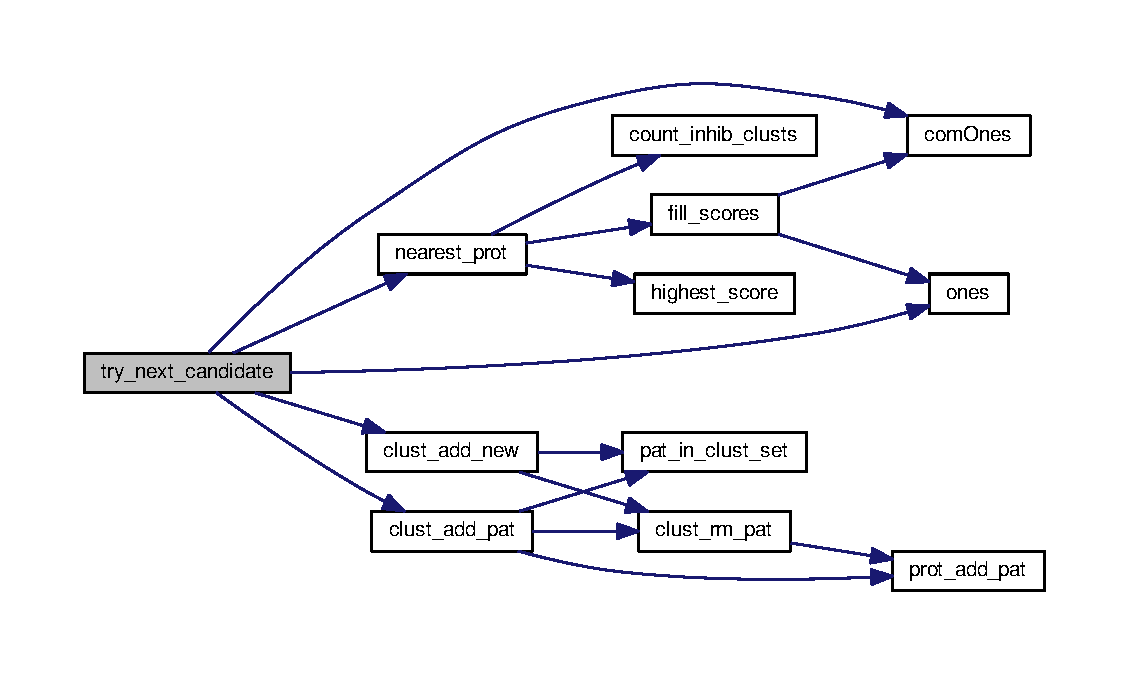
\includegraphics[width=350pt]{art1_8c_a3e69b8605f3c9eea5ef7aef29f5d5f05_cgraph}
\end{center}
\end{figure}




Here is the caller graph for this function\-:\nopagebreak
\begin{figure}[H]
\begin{center}
\leavevmode
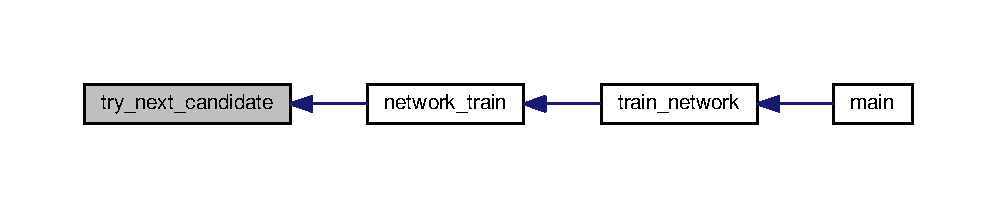
\includegraphics[width=350pt]{art1_8c_a3e69b8605f3c9eea5ef7aef29f5d5f05_icgraph}
\end{center}
\end{figure}



\hypertarget{art1_8h}{\section{src/art1.h File Reference}
\label{art1_8h}\index{src/art1.\-h@{src/art1.\-h}}
}
{\ttfamily \#include \char`\"{}utls.\-h\char`\"{}}\\*
Include dependency graph for art1.\-h\-:\nopagebreak
\begin{figure}[H]
\begin{center}
\leavevmode
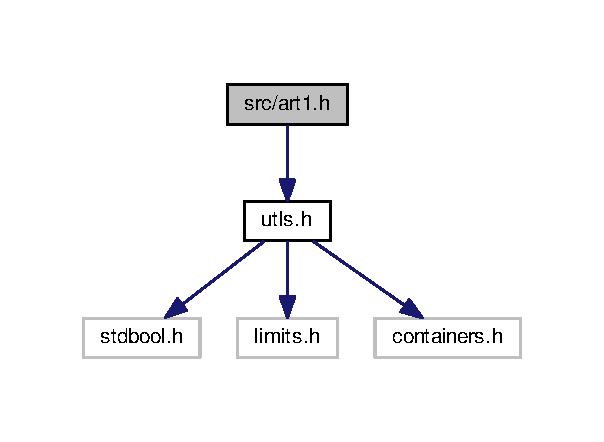
\includegraphics[width=290pt]{art1_8h__incl}
\end{center}
\end{figure}
This graph shows which files directly or indirectly include this file\-:\nopagebreak
\begin{figure}[H]
\begin{center}
\leavevmode
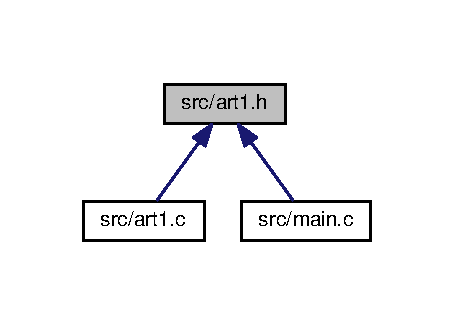
\includegraphics[width=218pt]{art1_8h__dep__incl}
\end{center}
\end{figure}
\subsection*{Macros}
\begin{DoxyCompactItemize}
\item 
\#define \hyperlink{art1_8h_a655c84af1b0034986ff56e12e84f983d}{N\-O\-N\-E}~-\/1
\end{DoxyCompactItemize}
\subsection*{Functions}
\begin{DoxyCompactItemize}
\item 
void \hyperlink{art1_8h_ae84af51b551ff2e1db27eb807d0c5522}{network\-\_\-train} (Vector $\ast$$\ast$best\-Clusts, float $\ast$best\-Fluc, \hyperlink{struct_in_param}{In\-Param} par, Vector $\ast$pats)
\item 
void \hyperlink{art1_8h_a117176d6a29f878cdc5030f70507868d}{network\-\_\-test} (Vector $\ast$$\ast$test\-Classes, Vector $\ast$best\-Clusts, \hyperlink{struct_in_param}{In\-Param} par, Vector $\ast$pats, Vector $\ast$clusts\-Classes, Vector $\ast$classes)
\end{DoxyCompactItemize}


\subsection{Macro Definition Documentation}
\hypertarget{art1_8h_a655c84af1b0034986ff56e12e84f983d}{\index{art1.\-h@{art1.\-h}!N\-O\-N\-E@{N\-O\-N\-E}}
\index{N\-O\-N\-E@{N\-O\-N\-E}!art1.h@{art1.\-h}}
\subsubsection[{N\-O\-N\-E}]{\setlength{\rightskip}{0pt plus 5cm}\#define N\-O\-N\-E~-\/1}}\label{art1_8h_a655c84af1b0034986ff56e12e84f983d}


\subsection{Function Documentation}
\hypertarget{art1_8h_a117176d6a29f878cdc5030f70507868d}{\index{art1.\-h@{art1.\-h}!network\-\_\-test@{network\-\_\-test}}
\index{network\-\_\-test@{network\-\_\-test}!art1.h@{art1.\-h}}
\subsubsection[{network\-\_\-test}]{\setlength{\rightskip}{0pt plus 5cm}void network\-\_\-test (
\begin{DoxyParamCaption}
\item[{Vector $\ast$$\ast$}]{test\-Classes, }
\item[{Vector $\ast$}]{best\-Clusts, }
\item[{{\bf In\-Param}}]{par, }
\item[{Vector $\ast$}]{pats, }
\item[{Vector $\ast$}]{clusts\-Classes, }
\item[{Vector $\ast$}]{classes}
\end{DoxyParamCaption}
)}}\label{art1_8h_a117176d6a29f878cdc5030f70507868d}


Here is the call graph for this function\-:\nopagebreak
\begin{figure}[H]
\begin{center}
\leavevmode
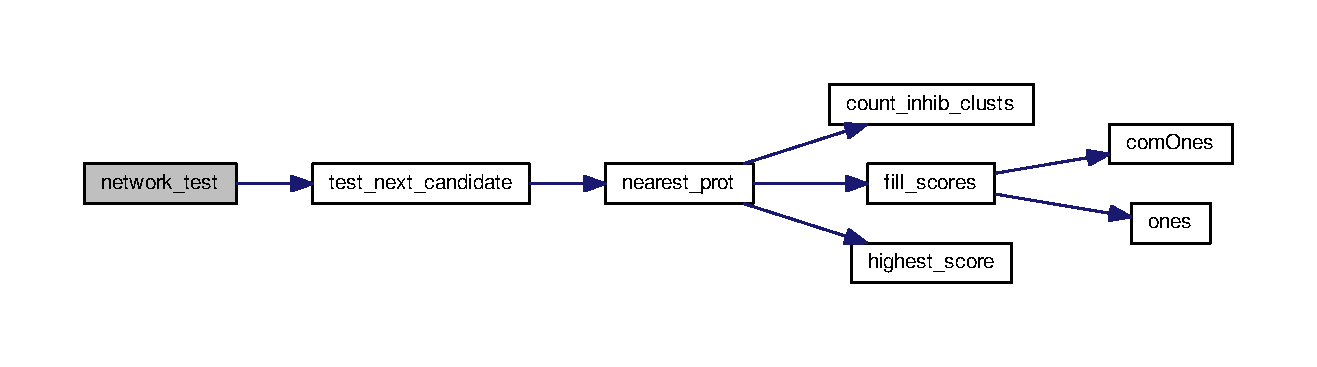
\includegraphics[width=350pt]{art1_8h_a117176d6a29f878cdc5030f70507868d_cgraph}
\end{center}
\end{figure}




Here is the caller graph for this function\-:\nopagebreak
\begin{figure}[H]
\begin{center}
\leavevmode
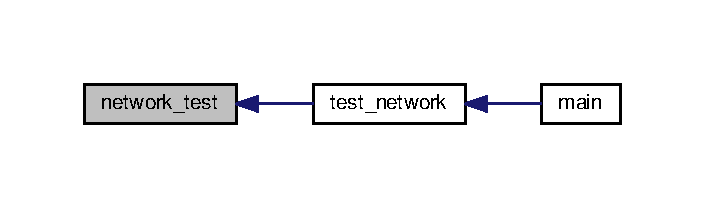
\includegraphics[width=338pt]{art1_8h_a117176d6a29f878cdc5030f70507868d_icgraph}
\end{center}
\end{figure}


\hypertarget{art1_8h_ae84af51b551ff2e1db27eb807d0c5522}{\index{art1.\-h@{art1.\-h}!network\-\_\-train@{network\-\_\-train}}
\index{network\-\_\-train@{network\-\_\-train}!art1.h@{art1.\-h}}
\subsubsection[{network\-\_\-train}]{\setlength{\rightskip}{0pt plus 5cm}void network\-\_\-train (
\begin{DoxyParamCaption}
\item[{Vector $\ast$$\ast$}]{best\-Clusts, }
\item[{float $\ast$}]{best\-Fluc, }
\item[{{\bf In\-Param}}]{par, }
\item[{Vector $\ast$}]{pats}
\end{DoxyParamCaption}
)}}\label{art1_8h_ae84af51b551ff2e1db27eb807d0c5522}
Train the network using the training patterns set and the parameters.

It loops until at least one stop condition is met. There's two stop conditions\-:
\begin{DoxyItemize}
\item Stop when the number of performed passes reaches the maximum number of passes (par-\/$>$max\-Passes).
\item Stop when the fluctuation rate is lower than or equal to the maximum fluctuation percentage (par-\/$>$min\-Fluc).
\end{DoxyItemize}

Inside this while loop there's a for loop which loops for each training patterns. And inside this for loop there's a second while loop which loops until the pattern is successfuly added to an existing or a new cluster.

The function looks like\-:\-:

L\-O\-O\-P W\-H\-I\-L\-E ( pass $<$ max\-Passes ) A\-N\-D ( fluc $>$ min\-Fluc )\-: L\-O\-O\-P F\-O\-R pat I\-N pats\-: D\-O\-: candidat = pick\-\_\-a\-\_\-candidat(clusters, pat) W\-H\-I\-L\-E N\-O\-T fits\-\_\-in\-\_\-candidat(candidat, pat)


\begin{DoxyParams}[1]{Parameters}
\mbox{\tt out}  & {\em best\-Clusts} & \\
\hline
\mbox{\tt out}  & {\em best\-Fluc} & \\
\hline
\mbox{\tt in}  & {\em pats} & \\
\hline
\mbox{\tt in}  & {\em par} & \\
\hline
\end{DoxyParams}


Here is the call graph for this function\-:\nopagebreak
\begin{figure}[H]
\begin{center}
\leavevmode
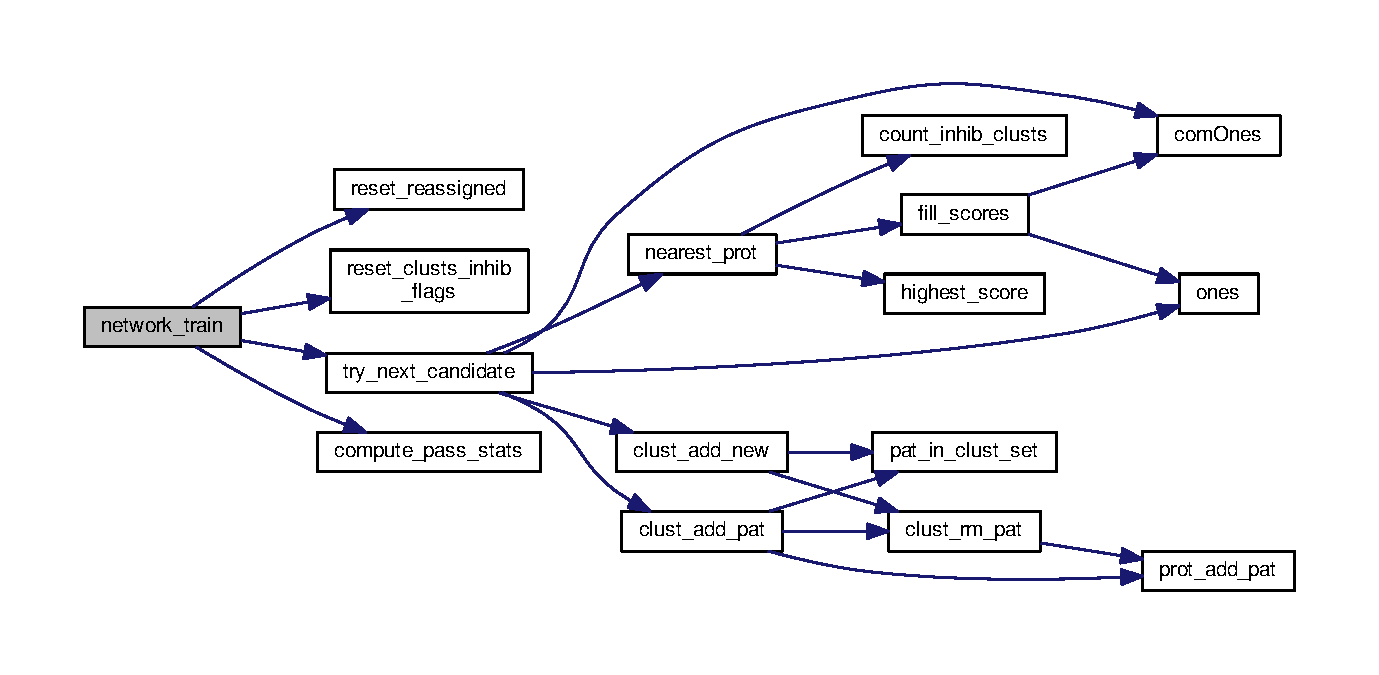
\includegraphics[width=350pt]{art1_8h_ae84af51b551ff2e1db27eb807d0c5522_cgraph}
\end{center}
\end{figure}




Here is the caller graph for this function\-:\nopagebreak
\begin{figure}[H]
\begin{center}
\leavevmode
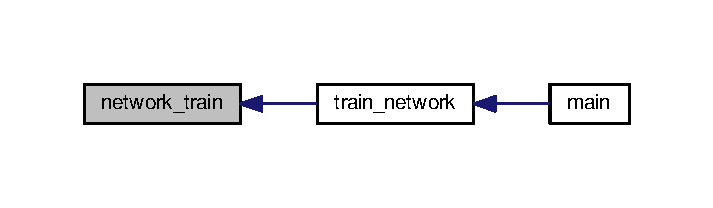
\includegraphics[width=342pt]{art1_8h_ae84af51b551ff2e1db27eb807d0c5522_icgraph}
\end{center}
\end{figure}



\hypertarget{dbg_8h}{\section{src/dbg.h File Reference}
\label{dbg_8h}\index{src/dbg.\-h@{src/dbg.\-h}}
}
{\ttfamily \#include $<$stdio.\-h$>$}\\*
{\ttfamily \#include $<$string.\-h$>$}\\*
Include dependency graph for dbg.\-h\-:\nopagebreak
\begin{figure}[H]
\begin{center}
\leavevmode
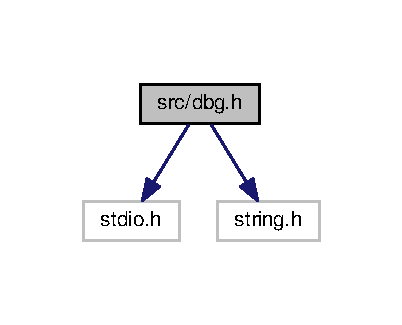
\includegraphics[width=193pt]{dbg_8h__incl}
\end{center}
\end{figure}
\subsection*{Macros}
\begin{DoxyCompactItemize}
\item 
\#define \hyperlink{dbg_8h_ad72dbcf6d0153db1b8d8a58001feed83}{D\-E\-B\-U\-G}~1
\item 
\#define \hyperlink{dbg_8h_ab117546549783a058d0321a287699579}{F\-I\-L\-E\-\_\-\-N\-A\-M\-E}~(strrchr(\-\_\-\-\_\-\-F\-I\-L\-E\-\_\-\-\_\-, '/') ? strrchr(\-\_\-\-\_\-\-F\-I\-L\-E\-\_\-\-\_\-, '/') + 1 \-: \-\_\-\-\_\-\-F\-I\-L\-E\-\_\-\-\_\-)
\item 
\#define \hyperlink{dbg_8h_a5f50bfe761aec48e94d11aa3a64e58a4}{D\-E\-B\-U\-G\-\_\-\-P\-R\-I\-N\-T}(fmt, args...)
\item 
\#define \hyperlink{dbg_8h_a328d67afea9e82f5abc2a841a85bbd29}{D\-E\-B\-U\-G\-\_\-\-P\-R\-I\-N\-T\-\_\-\-B\-L\-K}(fmt, args...)
\item 
\#define \hyperlink{dbg_8h_a21911df0bb1d23769725955c193db00d}{D\-E\-B\-U\-G\-\_\-\-P\-R\-I\-N\-T\-\_\-\-R\-E\-D}(fmt, args...)
\item 
\#define \hyperlink{dbg_8h_a4150ca1ead9e4fdbb8587923be86346b}{D\-E\-B\-U\-G\-\_\-\-P\-R\-I\-N\-T\-\_\-\-G\-R\-N}(fmt, args...)
\item 
\#define \hyperlink{dbg_8h_a6957d141d7726e6441e101b796428b6a}{D\-E\-B\-U\-G\-\_\-\-P\-R\-I\-N\-T\-\_\-\-Y\-E\-L}(fmt, args...)
\item 
\#define \hyperlink{dbg_8h_a7fbad654c940518f3b6c160dad36df90}{D\-E\-B\-U\-G\-\_\-\-P\-R\-I\-N\-T\-\_\-\-B\-L\-U}(fmt, args...)
\item 
\#define \hyperlink{dbg_8h_a065fb02a149e3da045cc7c894c16c437}{D\-E\-B\-U\-G\-\_\-\-P\-R\-I\-N\-T\-\_\-\-M\-A\-G}(fmt, args...)
\item 
\#define \hyperlink{dbg_8h_a3c7904f5a2f1a9231228db4908b4b812}{D\-E\-B\-U\-G\-\_\-\-P\-R\-I\-N\-T\-\_\-\-C\-Y\-N}(fmt, args...)
\item 
\#define \hyperlink{dbg_8h_af0e8b8aa6a54b920c639712a991092a1}{D\-E\-B\-U\-G\-\_\-\-P\-R\-I\-N\-T\-\_\-\-W\-H\-T}(fmt, args...)
\item 
\#define \hyperlink{dbg_8h_af26513079dd46b3981d6204ffed33ab1}{D\-E\-B\-U\-G\-\_\-\-P\-R\-I\-N\-T\-\_\-\-B\-N\-R\-M}(fmt, args...)
\item 
\#define \hyperlink{dbg_8h_a6a0c4e7139e04470e582f5d209b6bd19}{D\-E\-B\-U\-G\-\_\-\-P\-R\-I\-N\-T\-\_\-\-B\-B\-L\-K}(fmt, args...)
\item 
\#define \hyperlink{dbg_8h_adc3a64078ccc8c6d9c050c420842f90c}{D\-E\-B\-U\-G\-\_\-\-P\-R\-I\-N\-T\-\_\-\-B\-R\-E\-D}(fmt, args...)
\item 
\#define \hyperlink{dbg_8h_a7549a09403308ddfcfe4fd4cf8a4dc64}{D\-E\-B\-U\-G\-\_\-\-P\-R\-I\-N\-T\-\_\-\-B\-G\-R\-N}(fmt, args...)
\item 
\#define \hyperlink{dbg_8h_a9131a8ecda93e452c39060b96119aa02}{D\-E\-B\-U\-G\-\_\-\-P\-R\-I\-N\-T\-\_\-\-B\-Y\-E\-L}(fmt, args...)
\item 
\#define \hyperlink{dbg_8h_ad00c0ba2859ce89797117788b262e0b0}{D\-E\-B\-U\-G\-\_\-\-P\-R\-I\-N\-T\-\_\-\-B\-B\-L\-U}(fmt, args...)
\item 
\#define \hyperlink{dbg_8h_a681f14d822e96ba8e963e7544dc6547b}{D\-E\-B\-U\-G\-\_\-\-P\-R\-I\-N\-T\-\_\-\-B\-M\-A\-G}(fmt, args...)
\item 
\#define \hyperlink{dbg_8h_acc3b702fa83799e6957cb362755bd660}{D\-E\-B\-U\-G\-\_\-\-P\-R\-I\-N\-T\-\_\-\-B\-C\-Y\-N}(fmt, args...)
\item 
\#define \hyperlink{dbg_8h_a7795f5c17e2ec79578e2e6479adc7298}{D\-E\-B\-U\-G\-\_\-\-P\-R\-I\-N\-T\-\_\-\-B\-W\-H\-T}(fmt, args...)
\item 
\#define \hyperlink{dbg_8h_ad3ad1f26a6331824bf69eb4a48b5a932}{D\-E\-B\-U\-G\-\_\-\-P\-R\-I\-N\-T\-\_\-\-G\-R\-N\-\_\-\-L}(fmt, args...)
\item 
\#define \hyperlink{dbg_8h_a307d5f75a1d4862021fce10efe08649b}{D\-E\-B\-U\-G\-\_\-\-P\-R\-I\-N\-T\-\_\-\-L}(fmt, args...)~fprintf(stderr, \char`\"{}\char`\"{} fmt, \#\#args);
\item 
\#define \hyperlink{dbg_8h_a0b16486ffa03df3730acbbfd372a563f}{D\-E\-B\-U\-G\-\_\-\-P\-R\-I\-N\-T\-\_\-\-N\-L}(fmt, args...)
\item 
\#define \hyperlink{dbg_8h_a9f541fa00b650a07a7b7d420f960fd58}{C\-N\-R\-M}~\char`\"{}\textbackslash{}x1\-B\mbox{[}0m\char`\"{}
\item 
\#define \hyperlink{dbg_8h_aeebd32a3db86bed40c0e9b857af5574f}{C\-B\-L\-K}~\char`\"{}\textbackslash{}x1\-B\mbox{[}30m\char`\"{}
\item 
\#define \hyperlink{dbg_8h_ab93994c82cc32f5aaa86dc9fe39b3942}{C\-R\-E\-D}~\char`\"{}\textbackslash{}x1\-B\mbox{[}31m\char`\"{}
\item 
\#define \hyperlink{dbg_8h_a106b9f1df0722c47b7865fe3eb5e20e7}{C\-G\-R\-N}~\char`\"{}\textbackslash{}x1\-B\mbox{[}32m\char`\"{}
\item 
\#define \hyperlink{dbg_8h_aae917ceb13ecf0bd2128f658408c4339}{C\-Y\-E\-L}~\char`\"{}\textbackslash{}x1\-B\mbox{[}33m\char`\"{}
\item 
\#define \hyperlink{dbg_8h_a9102ff0836b098fbba474475aa0fb259}{C\-B\-L\-U}~\char`\"{}\textbackslash{}x1\-B\mbox{[}34m\char`\"{}
\item 
\#define \hyperlink{dbg_8h_a90e4aa451b27ddde03d994400ebf76e4}{C\-M\-A\-G}~\char`\"{}\textbackslash{}x1\-B\mbox{[}35m\char`\"{}
\item 
\#define \hyperlink{dbg_8h_a4952d2edac374fbe8457c41a0e2fecfc}{C\-C\-Y\-N}~\char`\"{}\textbackslash{}x1\-B\mbox{[}36m\char`\"{}
\item 
\#define \hyperlink{dbg_8h_a3acd22b1fe80d6d32e7fa03eceb9d285}{C\-W\-H\-T}~\char`\"{}\textbackslash{}x1\-B\mbox{[}37m\char`\"{}
\item 
\#define \hyperlink{dbg_8h_a742ec442801be8e7d8c397fac05aaa03}{B\-N\-R\-M}~\char`\"{}\textbackslash{}x1\-B\mbox{[}1m\textbackslash{}x1b\mbox{[}0m\char`\"{}
\item 
\#define \hyperlink{dbg_8h_ab3bdb5557ea3a8f7ed80a55ad301e09c}{B\-B\-L\-K}~\char`\"{}\textbackslash{}x1\-B\mbox{[}1m\textbackslash{}x1b\mbox{[}30m\char`\"{}
\item 
\#define \hyperlink{dbg_8h_a2adb4c9e293ac446897ccfac5a52d6c2}{B\-R\-E\-D}~\char`\"{}\textbackslash{}x1\-B\mbox{[}1m\textbackslash{}x1b\mbox{[}31m\char`\"{}
\item 
\#define \hyperlink{dbg_8h_a003f38f51e5f6972a6a0796bda4ca11c}{B\-G\-R\-N}~\char`\"{}\textbackslash{}x1\-B\mbox{[}1m\textbackslash{}x1b\mbox{[}32m\char`\"{}
\item 
\#define \hyperlink{dbg_8h_a9b526756196d7c0efa31bc8fe4e5f138}{B\-Y\-E\-L}~\char`\"{}\textbackslash{}x1\-B\mbox{[}1m\textbackslash{}x1b\mbox{[}33m\char`\"{}
\item 
\#define \hyperlink{dbg_8h_a9f40b3c1c240d5513da9f50685d5bf15}{B\-B\-L\-U}~\char`\"{}\textbackslash{}x1\-B\mbox{[}1m\textbackslash{}x1b\mbox{[}34m\char`\"{}
\item 
\#define \hyperlink{dbg_8h_af1bdc3f8928aa1589ef44e3578a09464}{B\-M\-A\-G}~\char`\"{}\textbackslash{}x1\-B\mbox{[}1m\textbackslash{}x1b\mbox{[}35m\char`\"{}
\item 
\#define \hyperlink{dbg_8h_abd610b309fe5845f1e5fbd6666a22447}{B\-C\-Y\-N}~\char`\"{}\textbackslash{}x1\-B\mbox{[}1m\textbackslash{}x1b\mbox{[}36m\char`\"{}
\item 
\#define \hyperlink{dbg_8h_ae528cad0e6c76be71eb66776599ec5d9}{B\-W\-H\-T}~\char`\"{}\textbackslash{}x1\-B\mbox{[}1m\textbackslash{}x1b\mbox{[}37m\char`\"{}
\item 
\#define \hyperlink{dbg_8h_abd06b31226dd4cce571aa78694be60de}{B\-C\-R\-E\-D}~\char`\"{}\textbackslash{}x1\-B\mbox{[}41m\char`\"{}
\item 
\#define \hyperlink{dbg_8h_a17e568d7648c5aa948163e72d4c49e54}{B\-C\-G\-R\-N}~\char`\"{}\textbackslash{}x1\-B\mbox{[}42m\char`\"{}
\item 
\#define \hyperlink{dbg_8h_ade204fec1b7b1201feb4ea66769d2c8f}{B\-C\-W\-H\-T}~\char`\"{}\textbackslash{}x1\-B\mbox{[}47m\char`\"{}
\end{DoxyCompactItemize}


\subsection{Macro Definition Documentation}
\hypertarget{dbg_8h_ab3bdb5557ea3a8f7ed80a55ad301e09c}{\index{dbg.\-h@{dbg.\-h}!B\-B\-L\-K@{B\-B\-L\-K}}
\index{B\-B\-L\-K@{B\-B\-L\-K}!dbg.h@{dbg.\-h}}
\subsubsection[{B\-B\-L\-K}]{\setlength{\rightskip}{0pt plus 5cm}\#define B\-B\-L\-K~\char`\"{}\textbackslash{}x1\-B\mbox{[}1m\textbackslash{}x1b\mbox{[}30m\char`\"{}}}\label{dbg_8h_ab3bdb5557ea3a8f7ed80a55ad301e09c}
\hypertarget{dbg_8h_a9f40b3c1c240d5513da9f50685d5bf15}{\index{dbg.\-h@{dbg.\-h}!B\-B\-L\-U@{B\-B\-L\-U}}
\index{B\-B\-L\-U@{B\-B\-L\-U}!dbg.h@{dbg.\-h}}
\subsubsection[{B\-B\-L\-U}]{\setlength{\rightskip}{0pt plus 5cm}\#define B\-B\-L\-U~\char`\"{}\textbackslash{}x1\-B\mbox{[}1m\textbackslash{}x1b\mbox{[}34m\char`\"{}}}\label{dbg_8h_a9f40b3c1c240d5513da9f50685d5bf15}
\hypertarget{dbg_8h_a17e568d7648c5aa948163e72d4c49e54}{\index{dbg.\-h@{dbg.\-h}!B\-C\-G\-R\-N@{B\-C\-G\-R\-N}}
\index{B\-C\-G\-R\-N@{B\-C\-G\-R\-N}!dbg.h@{dbg.\-h}}
\subsubsection[{B\-C\-G\-R\-N}]{\setlength{\rightskip}{0pt plus 5cm}\#define B\-C\-G\-R\-N~\char`\"{}\textbackslash{}x1\-B\mbox{[}42m\char`\"{}}}\label{dbg_8h_a17e568d7648c5aa948163e72d4c49e54}
\hypertarget{dbg_8h_abd06b31226dd4cce571aa78694be60de}{\index{dbg.\-h@{dbg.\-h}!B\-C\-R\-E\-D@{B\-C\-R\-E\-D}}
\index{B\-C\-R\-E\-D@{B\-C\-R\-E\-D}!dbg.h@{dbg.\-h}}
\subsubsection[{B\-C\-R\-E\-D}]{\setlength{\rightskip}{0pt plus 5cm}\#define B\-C\-R\-E\-D~\char`\"{}\textbackslash{}x1\-B\mbox{[}41m\char`\"{}}}\label{dbg_8h_abd06b31226dd4cce571aa78694be60de}
\hypertarget{dbg_8h_ade204fec1b7b1201feb4ea66769d2c8f}{\index{dbg.\-h@{dbg.\-h}!B\-C\-W\-H\-T@{B\-C\-W\-H\-T}}
\index{B\-C\-W\-H\-T@{B\-C\-W\-H\-T}!dbg.h@{dbg.\-h}}
\subsubsection[{B\-C\-W\-H\-T}]{\setlength{\rightskip}{0pt plus 5cm}\#define B\-C\-W\-H\-T~\char`\"{}\textbackslash{}x1\-B\mbox{[}47m\char`\"{}}}\label{dbg_8h_ade204fec1b7b1201feb4ea66769d2c8f}
\hypertarget{dbg_8h_abd610b309fe5845f1e5fbd6666a22447}{\index{dbg.\-h@{dbg.\-h}!B\-C\-Y\-N@{B\-C\-Y\-N}}
\index{B\-C\-Y\-N@{B\-C\-Y\-N}!dbg.h@{dbg.\-h}}
\subsubsection[{B\-C\-Y\-N}]{\setlength{\rightskip}{0pt plus 5cm}\#define B\-C\-Y\-N~\char`\"{}\textbackslash{}x1\-B\mbox{[}1m\textbackslash{}x1b\mbox{[}36m\char`\"{}}}\label{dbg_8h_abd610b309fe5845f1e5fbd6666a22447}
\hypertarget{dbg_8h_a003f38f51e5f6972a6a0796bda4ca11c}{\index{dbg.\-h@{dbg.\-h}!B\-G\-R\-N@{B\-G\-R\-N}}
\index{B\-G\-R\-N@{B\-G\-R\-N}!dbg.h@{dbg.\-h}}
\subsubsection[{B\-G\-R\-N}]{\setlength{\rightskip}{0pt plus 5cm}\#define B\-G\-R\-N~\char`\"{}\textbackslash{}x1\-B\mbox{[}1m\textbackslash{}x1b\mbox{[}32m\char`\"{}}}\label{dbg_8h_a003f38f51e5f6972a6a0796bda4ca11c}
\hypertarget{dbg_8h_af1bdc3f8928aa1589ef44e3578a09464}{\index{dbg.\-h@{dbg.\-h}!B\-M\-A\-G@{B\-M\-A\-G}}
\index{B\-M\-A\-G@{B\-M\-A\-G}!dbg.h@{dbg.\-h}}
\subsubsection[{B\-M\-A\-G}]{\setlength{\rightskip}{0pt plus 5cm}\#define B\-M\-A\-G~\char`\"{}\textbackslash{}x1\-B\mbox{[}1m\textbackslash{}x1b\mbox{[}35m\char`\"{}}}\label{dbg_8h_af1bdc3f8928aa1589ef44e3578a09464}
\hypertarget{dbg_8h_a742ec442801be8e7d8c397fac05aaa03}{\index{dbg.\-h@{dbg.\-h}!B\-N\-R\-M@{B\-N\-R\-M}}
\index{B\-N\-R\-M@{B\-N\-R\-M}!dbg.h@{dbg.\-h}}
\subsubsection[{B\-N\-R\-M}]{\setlength{\rightskip}{0pt plus 5cm}\#define B\-N\-R\-M~\char`\"{}\textbackslash{}x1\-B\mbox{[}1m\textbackslash{}x1b\mbox{[}0m\char`\"{}}}\label{dbg_8h_a742ec442801be8e7d8c397fac05aaa03}
\hypertarget{dbg_8h_a2adb4c9e293ac446897ccfac5a52d6c2}{\index{dbg.\-h@{dbg.\-h}!B\-R\-E\-D@{B\-R\-E\-D}}
\index{B\-R\-E\-D@{B\-R\-E\-D}!dbg.h@{dbg.\-h}}
\subsubsection[{B\-R\-E\-D}]{\setlength{\rightskip}{0pt plus 5cm}\#define B\-R\-E\-D~\char`\"{}\textbackslash{}x1\-B\mbox{[}1m\textbackslash{}x1b\mbox{[}31m\char`\"{}}}\label{dbg_8h_a2adb4c9e293ac446897ccfac5a52d6c2}
\hypertarget{dbg_8h_ae528cad0e6c76be71eb66776599ec5d9}{\index{dbg.\-h@{dbg.\-h}!B\-W\-H\-T@{B\-W\-H\-T}}
\index{B\-W\-H\-T@{B\-W\-H\-T}!dbg.h@{dbg.\-h}}
\subsubsection[{B\-W\-H\-T}]{\setlength{\rightskip}{0pt plus 5cm}\#define B\-W\-H\-T~\char`\"{}\textbackslash{}x1\-B\mbox{[}1m\textbackslash{}x1b\mbox{[}37m\char`\"{}}}\label{dbg_8h_ae528cad0e6c76be71eb66776599ec5d9}
\hypertarget{dbg_8h_a9b526756196d7c0efa31bc8fe4e5f138}{\index{dbg.\-h@{dbg.\-h}!B\-Y\-E\-L@{B\-Y\-E\-L}}
\index{B\-Y\-E\-L@{B\-Y\-E\-L}!dbg.h@{dbg.\-h}}
\subsubsection[{B\-Y\-E\-L}]{\setlength{\rightskip}{0pt plus 5cm}\#define B\-Y\-E\-L~\char`\"{}\textbackslash{}x1\-B\mbox{[}1m\textbackslash{}x1b\mbox{[}33m\char`\"{}}}\label{dbg_8h_a9b526756196d7c0efa31bc8fe4e5f138}
\hypertarget{dbg_8h_aeebd32a3db86bed40c0e9b857af5574f}{\index{dbg.\-h@{dbg.\-h}!C\-B\-L\-K@{C\-B\-L\-K}}
\index{C\-B\-L\-K@{C\-B\-L\-K}!dbg.h@{dbg.\-h}}
\subsubsection[{C\-B\-L\-K}]{\setlength{\rightskip}{0pt plus 5cm}\#define C\-B\-L\-K~\char`\"{}\textbackslash{}x1\-B\mbox{[}30m\char`\"{}}}\label{dbg_8h_aeebd32a3db86bed40c0e9b857af5574f}
\hypertarget{dbg_8h_a9102ff0836b098fbba474475aa0fb259}{\index{dbg.\-h@{dbg.\-h}!C\-B\-L\-U@{C\-B\-L\-U}}
\index{C\-B\-L\-U@{C\-B\-L\-U}!dbg.h@{dbg.\-h}}
\subsubsection[{C\-B\-L\-U}]{\setlength{\rightskip}{0pt plus 5cm}\#define C\-B\-L\-U~\char`\"{}\textbackslash{}x1\-B\mbox{[}34m\char`\"{}}}\label{dbg_8h_a9102ff0836b098fbba474475aa0fb259}
\hypertarget{dbg_8h_a4952d2edac374fbe8457c41a0e2fecfc}{\index{dbg.\-h@{dbg.\-h}!C\-C\-Y\-N@{C\-C\-Y\-N}}
\index{C\-C\-Y\-N@{C\-C\-Y\-N}!dbg.h@{dbg.\-h}}
\subsubsection[{C\-C\-Y\-N}]{\setlength{\rightskip}{0pt plus 5cm}\#define C\-C\-Y\-N~\char`\"{}\textbackslash{}x1\-B\mbox{[}36m\char`\"{}}}\label{dbg_8h_a4952d2edac374fbe8457c41a0e2fecfc}
\hypertarget{dbg_8h_a106b9f1df0722c47b7865fe3eb5e20e7}{\index{dbg.\-h@{dbg.\-h}!C\-G\-R\-N@{C\-G\-R\-N}}
\index{C\-G\-R\-N@{C\-G\-R\-N}!dbg.h@{dbg.\-h}}
\subsubsection[{C\-G\-R\-N}]{\setlength{\rightskip}{0pt plus 5cm}\#define C\-G\-R\-N~\char`\"{}\textbackslash{}x1\-B\mbox{[}32m\char`\"{}}}\label{dbg_8h_a106b9f1df0722c47b7865fe3eb5e20e7}
\hypertarget{dbg_8h_a90e4aa451b27ddde03d994400ebf76e4}{\index{dbg.\-h@{dbg.\-h}!C\-M\-A\-G@{C\-M\-A\-G}}
\index{C\-M\-A\-G@{C\-M\-A\-G}!dbg.h@{dbg.\-h}}
\subsubsection[{C\-M\-A\-G}]{\setlength{\rightskip}{0pt plus 5cm}\#define C\-M\-A\-G~\char`\"{}\textbackslash{}x1\-B\mbox{[}35m\char`\"{}}}\label{dbg_8h_a90e4aa451b27ddde03d994400ebf76e4}
\hypertarget{dbg_8h_a9f541fa00b650a07a7b7d420f960fd58}{\index{dbg.\-h@{dbg.\-h}!C\-N\-R\-M@{C\-N\-R\-M}}
\index{C\-N\-R\-M@{C\-N\-R\-M}!dbg.h@{dbg.\-h}}
\subsubsection[{C\-N\-R\-M}]{\setlength{\rightskip}{0pt plus 5cm}\#define C\-N\-R\-M~\char`\"{}\textbackslash{}x1\-B\mbox{[}0m\char`\"{}}}\label{dbg_8h_a9f541fa00b650a07a7b7d420f960fd58}
\hypertarget{dbg_8h_ab93994c82cc32f5aaa86dc9fe39b3942}{\index{dbg.\-h@{dbg.\-h}!C\-R\-E\-D@{C\-R\-E\-D}}
\index{C\-R\-E\-D@{C\-R\-E\-D}!dbg.h@{dbg.\-h}}
\subsubsection[{C\-R\-E\-D}]{\setlength{\rightskip}{0pt plus 5cm}\#define C\-R\-E\-D~\char`\"{}\textbackslash{}x1\-B\mbox{[}31m\char`\"{}}}\label{dbg_8h_ab93994c82cc32f5aaa86dc9fe39b3942}
\hypertarget{dbg_8h_a3acd22b1fe80d6d32e7fa03eceb9d285}{\index{dbg.\-h@{dbg.\-h}!C\-W\-H\-T@{C\-W\-H\-T}}
\index{C\-W\-H\-T@{C\-W\-H\-T}!dbg.h@{dbg.\-h}}
\subsubsection[{C\-W\-H\-T}]{\setlength{\rightskip}{0pt plus 5cm}\#define C\-W\-H\-T~\char`\"{}\textbackslash{}x1\-B\mbox{[}37m\char`\"{}}}\label{dbg_8h_a3acd22b1fe80d6d32e7fa03eceb9d285}
\hypertarget{dbg_8h_aae917ceb13ecf0bd2128f658408c4339}{\index{dbg.\-h@{dbg.\-h}!C\-Y\-E\-L@{C\-Y\-E\-L}}
\index{C\-Y\-E\-L@{C\-Y\-E\-L}!dbg.h@{dbg.\-h}}
\subsubsection[{C\-Y\-E\-L}]{\setlength{\rightskip}{0pt plus 5cm}\#define C\-Y\-E\-L~\char`\"{}\textbackslash{}x1\-B\mbox{[}33m\char`\"{}}}\label{dbg_8h_aae917ceb13ecf0bd2128f658408c4339}
\hypertarget{dbg_8h_ad72dbcf6d0153db1b8d8a58001feed83}{\index{dbg.\-h@{dbg.\-h}!D\-E\-B\-U\-G@{D\-E\-B\-U\-G}}
\index{D\-E\-B\-U\-G@{D\-E\-B\-U\-G}!dbg.h@{dbg.\-h}}
\subsubsection[{D\-E\-B\-U\-G}]{\setlength{\rightskip}{0pt plus 5cm}\#define D\-E\-B\-U\-G~1}}\label{dbg_8h_ad72dbcf6d0153db1b8d8a58001feed83}
\hypertarget{dbg_8h_a5f50bfe761aec48e94d11aa3a64e58a4}{\index{dbg.\-h@{dbg.\-h}!D\-E\-B\-U\-G\-\_\-\-P\-R\-I\-N\-T@{D\-E\-B\-U\-G\-\_\-\-P\-R\-I\-N\-T}}
\index{D\-E\-B\-U\-G\-\_\-\-P\-R\-I\-N\-T@{D\-E\-B\-U\-G\-\_\-\-P\-R\-I\-N\-T}!dbg.h@{dbg.\-h}}
\subsubsection[{D\-E\-B\-U\-G\-\_\-\-P\-R\-I\-N\-T}]{\setlength{\rightskip}{0pt plus 5cm}\#define D\-E\-B\-U\-G\-\_\-\-P\-R\-I\-N\-T(
\begin{DoxyParamCaption}
\item[{}]{fmt, }
\item[{}]{args...}
\end{DoxyParamCaption}
)}}\label{dbg_8h_a5f50bfe761aec48e94d11aa3a64e58a4}
{\bfseries Value\-:}
\begin{DoxyCode}
fprintf(stderr, \textcolor{stringliteral}{"%sDEBUG:%s %s:%d:%s(): %s"} fmt,\(\backslash\)
                \hyperlink{dbg_8h_ab93994c82cc32f5aaa86dc9fe39b3942}{CRED}, \hyperlink{dbg_8h_a9f541fa00b650a07a7b7d420f960fd58}{CNRM}, \hyperlink{dbg_8h_ab117546549783a058d0321a287699579}{FILE\_NAME}, \_\_LINE\_\_, \_\_func\_\_, \hyperlink{dbg_8h_a9f541fa00b650a07a7b7d420f960fd58}{CNRM}, ##args);\(\backslash\)
        fprintf(stderr, \textcolor{stringliteral}{"%s\(\backslash\)n"}, \hyperlink{dbg_8h_a9f541fa00b650a07a7b7d420f960fd58}{CNRM});
\end{DoxyCode}
\hypertarget{dbg_8h_a6a0c4e7139e04470e582f5d209b6bd19}{\index{dbg.\-h@{dbg.\-h}!D\-E\-B\-U\-G\-\_\-\-P\-R\-I\-N\-T\-\_\-\-B\-B\-L\-K@{D\-E\-B\-U\-G\-\_\-\-P\-R\-I\-N\-T\-\_\-\-B\-B\-L\-K}}
\index{D\-E\-B\-U\-G\-\_\-\-P\-R\-I\-N\-T\-\_\-\-B\-B\-L\-K@{D\-E\-B\-U\-G\-\_\-\-P\-R\-I\-N\-T\-\_\-\-B\-B\-L\-K}!dbg.h@{dbg.\-h}}
\subsubsection[{D\-E\-B\-U\-G\-\_\-\-P\-R\-I\-N\-T\-\_\-\-B\-B\-L\-K}]{\setlength{\rightskip}{0pt plus 5cm}\#define D\-E\-B\-U\-G\-\_\-\-P\-R\-I\-N\-T\-\_\-\-B\-B\-L\-K(
\begin{DoxyParamCaption}
\item[{}]{fmt, }
\item[{}]{args...}
\end{DoxyParamCaption}
)}}\label{dbg_8h_a6a0c4e7139e04470e582f5d209b6bd19}
{\bfseries Value\-:}
\begin{DoxyCode}
fprintf(stderr, \textcolor{stringliteral}{"%sDEBUG:%s %s:%d:%s(): %s"} fmt,\(\backslash\)
                \hyperlink{dbg_8h_ab93994c82cc32f5aaa86dc9fe39b3942}{CRED}, \hyperlink{dbg_8h_ab3bdb5557ea3a8f7ed80a55ad301e09c}{BBLK}, \hyperlink{dbg_8h_ab117546549783a058d0321a287699579}{FILE\_NAME}, \_\_LINE\_\_, \_\_func\_\_, \hyperlink{dbg_8h_a9f541fa00b650a07a7b7d420f960fd58}{CNRM}, ##args);\(\backslash\)
        fprintf(stderr, \textcolor{stringliteral}{"%s\(\backslash\)n"}, \hyperlink{dbg_8h_a9f541fa00b650a07a7b7d420f960fd58}{CNRM});
\end{DoxyCode}
\hypertarget{dbg_8h_ad00c0ba2859ce89797117788b262e0b0}{\index{dbg.\-h@{dbg.\-h}!D\-E\-B\-U\-G\-\_\-\-P\-R\-I\-N\-T\-\_\-\-B\-B\-L\-U@{D\-E\-B\-U\-G\-\_\-\-P\-R\-I\-N\-T\-\_\-\-B\-B\-L\-U}}
\index{D\-E\-B\-U\-G\-\_\-\-P\-R\-I\-N\-T\-\_\-\-B\-B\-L\-U@{D\-E\-B\-U\-G\-\_\-\-P\-R\-I\-N\-T\-\_\-\-B\-B\-L\-U}!dbg.h@{dbg.\-h}}
\subsubsection[{D\-E\-B\-U\-G\-\_\-\-P\-R\-I\-N\-T\-\_\-\-B\-B\-L\-U}]{\setlength{\rightskip}{0pt plus 5cm}\#define D\-E\-B\-U\-G\-\_\-\-P\-R\-I\-N\-T\-\_\-\-B\-B\-L\-U(
\begin{DoxyParamCaption}
\item[{}]{fmt, }
\item[{}]{args...}
\end{DoxyParamCaption}
)}}\label{dbg_8h_ad00c0ba2859ce89797117788b262e0b0}
{\bfseries Value\-:}
\begin{DoxyCode}
fprintf(stderr, \textcolor{stringliteral}{"%sDEBUG:%s %s:%d:%s(): %s"} fmt,\(\backslash\)
                \hyperlink{dbg_8h_ab93994c82cc32f5aaa86dc9fe39b3942}{CRED}, \hyperlink{dbg_8h_a9f40b3c1c240d5513da9f50685d5bf15}{BBLU}, \hyperlink{dbg_8h_ab117546549783a058d0321a287699579}{FILE\_NAME}, \_\_LINE\_\_, \_\_func\_\_, \hyperlink{dbg_8h_a9f541fa00b650a07a7b7d420f960fd58}{CNRM}, ##args);\(\backslash\)
        fprintf(stderr, \textcolor{stringliteral}{"%s\(\backslash\)n"}, \hyperlink{dbg_8h_a9f541fa00b650a07a7b7d420f960fd58}{CNRM});
\end{DoxyCode}
\hypertarget{dbg_8h_acc3b702fa83799e6957cb362755bd660}{\index{dbg.\-h@{dbg.\-h}!D\-E\-B\-U\-G\-\_\-\-P\-R\-I\-N\-T\-\_\-\-B\-C\-Y\-N@{D\-E\-B\-U\-G\-\_\-\-P\-R\-I\-N\-T\-\_\-\-B\-C\-Y\-N}}
\index{D\-E\-B\-U\-G\-\_\-\-P\-R\-I\-N\-T\-\_\-\-B\-C\-Y\-N@{D\-E\-B\-U\-G\-\_\-\-P\-R\-I\-N\-T\-\_\-\-B\-C\-Y\-N}!dbg.h@{dbg.\-h}}
\subsubsection[{D\-E\-B\-U\-G\-\_\-\-P\-R\-I\-N\-T\-\_\-\-B\-C\-Y\-N}]{\setlength{\rightskip}{0pt plus 5cm}\#define D\-E\-B\-U\-G\-\_\-\-P\-R\-I\-N\-T\-\_\-\-B\-C\-Y\-N(
\begin{DoxyParamCaption}
\item[{}]{fmt, }
\item[{}]{args...}
\end{DoxyParamCaption}
)}}\label{dbg_8h_acc3b702fa83799e6957cb362755bd660}
{\bfseries Value\-:}
\begin{DoxyCode}
fprintf(stderr, \textcolor{stringliteral}{"%sDEBUG:%s %s:%d:%s(): %s"} fmt,\(\backslash\)
                \hyperlink{dbg_8h_ab93994c82cc32f5aaa86dc9fe39b3942}{CRED}, \hyperlink{dbg_8h_abd610b309fe5845f1e5fbd6666a22447}{BCYN}, \hyperlink{dbg_8h_ab117546549783a058d0321a287699579}{FILE\_NAME}, \_\_LINE\_\_, \_\_func\_\_, \hyperlink{dbg_8h_a9f541fa00b650a07a7b7d420f960fd58}{CNRM}, ##args);\(\backslash\)
        fprintf(stderr, \textcolor{stringliteral}{"%s\(\backslash\)n"}, \hyperlink{dbg_8h_a9f541fa00b650a07a7b7d420f960fd58}{CNRM});
\end{DoxyCode}
\hypertarget{dbg_8h_a7549a09403308ddfcfe4fd4cf8a4dc64}{\index{dbg.\-h@{dbg.\-h}!D\-E\-B\-U\-G\-\_\-\-P\-R\-I\-N\-T\-\_\-\-B\-G\-R\-N@{D\-E\-B\-U\-G\-\_\-\-P\-R\-I\-N\-T\-\_\-\-B\-G\-R\-N}}
\index{D\-E\-B\-U\-G\-\_\-\-P\-R\-I\-N\-T\-\_\-\-B\-G\-R\-N@{D\-E\-B\-U\-G\-\_\-\-P\-R\-I\-N\-T\-\_\-\-B\-G\-R\-N}!dbg.h@{dbg.\-h}}
\subsubsection[{D\-E\-B\-U\-G\-\_\-\-P\-R\-I\-N\-T\-\_\-\-B\-G\-R\-N}]{\setlength{\rightskip}{0pt plus 5cm}\#define D\-E\-B\-U\-G\-\_\-\-P\-R\-I\-N\-T\-\_\-\-B\-G\-R\-N(
\begin{DoxyParamCaption}
\item[{}]{fmt, }
\item[{}]{args...}
\end{DoxyParamCaption}
)}}\label{dbg_8h_a7549a09403308ddfcfe4fd4cf8a4dc64}
{\bfseries Value\-:}
\begin{DoxyCode}
fprintf(stderr, \textcolor{stringliteral}{"%sDEBUG:%s %s:%d:%s(): %s"} fmt,\(\backslash\)
                \hyperlink{dbg_8h_ab93994c82cc32f5aaa86dc9fe39b3942}{CRED}, \hyperlink{dbg_8h_a003f38f51e5f6972a6a0796bda4ca11c}{BGRN}, \hyperlink{dbg_8h_ab117546549783a058d0321a287699579}{FILE\_NAME}, \_\_LINE\_\_, \_\_func\_\_, \hyperlink{dbg_8h_a9f541fa00b650a07a7b7d420f960fd58}{CNRM}, ##args);\(\backslash\)
        fprintf(stderr, \textcolor{stringliteral}{"%s\(\backslash\)n"}, \hyperlink{dbg_8h_a9f541fa00b650a07a7b7d420f960fd58}{CNRM});
\end{DoxyCode}
\hypertarget{dbg_8h_a328d67afea9e82f5abc2a841a85bbd29}{\index{dbg.\-h@{dbg.\-h}!D\-E\-B\-U\-G\-\_\-\-P\-R\-I\-N\-T\-\_\-\-B\-L\-K@{D\-E\-B\-U\-G\-\_\-\-P\-R\-I\-N\-T\-\_\-\-B\-L\-K}}
\index{D\-E\-B\-U\-G\-\_\-\-P\-R\-I\-N\-T\-\_\-\-B\-L\-K@{D\-E\-B\-U\-G\-\_\-\-P\-R\-I\-N\-T\-\_\-\-B\-L\-K}!dbg.h@{dbg.\-h}}
\subsubsection[{D\-E\-B\-U\-G\-\_\-\-P\-R\-I\-N\-T\-\_\-\-B\-L\-K}]{\setlength{\rightskip}{0pt plus 5cm}\#define D\-E\-B\-U\-G\-\_\-\-P\-R\-I\-N\-T\-\_\-\-B\-L\-K(
\begin{DoxyParamCaption}
\item[{}]{fmt, }
\item[{}]{args...}
\end{DoxyParamCaption}
)}}\label{dbg_8h_a328d67afea9e82f5abc2a841a85bbd29}
{\bfseries Value\-:}
\begin{DoxyCode}
fprintf(stderr, \textcolor{stringliteral}{"%sDEBUG:%s %s:%d:%s(): %s"} fmt,\(\backslash\)
                \hyperlink{dbg_8h_ab93994c82cc32f5aaa86dc9fe39b3942}{CRED}, \hyperlink{dbg_8h_aeebd32a3db86bed40c0e9b857af5574f}{CBLK}, \hyperlink{dbg_8h_ab117546549783a058d0321a287699579}{FILE\_NAME}, \_\_LINE\_\_, \_\_func\_\_, \hyperlink{dbg_8h_a9f541fa00b650a07a7b7d420f960fd58}{CNRM}, ##args);\(\backslash\)
        fprintf(stderr, \textcolor{stringliteral}{"%s\(\backslash\)n"}, \hyperlink{dbg_8h_a9f541fa00b650a07a7b7d420f960fd58}{CNRM});
\end{DoxyCode}
\hypertarget{dbg_8h_a7fbad654c940518f3b6c160dad36df90}{\index{dbg.\-h@{dbg.\-h}!D\-E\-B\-U\-G\-\_\-\-P\-R\-I\-N\-T\-\_\-\-B\-L\-U@{D\-E\-B\-U\-G\-\_\-\-P\-R\-I\-N\-T\-\_\-\-B\-L\-U}}
\index{D\-E\-B\-U\-G\-\_\-\-P\-R\-I\-N\-T\-\_\-\-B\-L\-U@{D\-E\-B\-U\-G\-\_\-\-P\-R\-I\-N\-T\-\_\-\-B\-L\-U}!dbg.h@{dbg.\-h}}
\subsubsection[{D\-E\-B\-U\-G\-\_\-\-P\-R\-I\-N\-T\-\_\-\-B\-L\-U}]{\setlength{\rightskip}{0pt plus 5cm}\#define D\-E\-B\-U\-G\-\_\-\-P\-R\-I\-N\-T\-\_\-\-B\-L\-U(
\begin{DoxyParamCaption}
\item[{}]{fmt, }
\item[{}]{args...}
\end{DoxyParamCaption}
)}}\label{dbg_8h_a7fbad654c940518f3b6c160dad36df90}
{\bfseries Value\-:}
\begin{DoxyCode}
fprintf(stderr, \textcolor{stringliteral}{"%sDEBUG:%s %s:%d:%s(): %s"} fmt,\(\backslash\)
                \hyperlink{dbg_8h_ab93994c82cc32f5aaa86dc9fe39b3942}{CRED}, \hyperlink{dbg_8h_a9102ff0836b098fbba474475aa0fb259}{CBLU}, \hyperlink{dbg_8h_ab117546549783a058d0321a287699579}{FILE\_NAME}, \_\_LINE\_\_, \_\_func\_\_, \hyperlink{dbg_8h_a9f541fa00b650a07a7b7d420f960fd58}{CNRM}, ##args);\(\backslash\)
        fprintf(stderr, \textcolor{stringliteral}{"%s\(\backslash\)n"}, \hyperlink{dbg_8h_a9f541fa00b650a07a7b7d420f960fd58}{CNRM});
\end{DoxyCode}
\hypertarget{dbg_8h_a681f14d822e96ba8e963e7544dc6547b}{\index{dbg.\-h@{dbg.\-h}!D\-E\-B\-U\-G\-\_\-\-P\-R\-I\-N\-T\-\_\-\-B\-M\-A\-G@{D\-E\-B\-U\-G\-\_\-\-P\-R\-I\-N\-T\-\_\-\-B\-M\-A\-G}}
\index{D\-E\-B\-U\-G\-\_\-\-P\-R\-I\-N\-T\-\_\-\-B\-M\-A\-G@{D\-E\-B\-U\-G\-\_\-\-P\-R\-I\-N\-T\-\_\-\-B\-M\-A\-G}!dbg.h@{dbg.\-h}}
\subsubsection[{D\-E\-B\-U\-G\-\_\-\-P\-R\-I\-N\-T\-\_\-\-B\-M\-A\-G}]{\setlength{\rightskip}{0pt plus 5cm}\#define D\-E\-B\-U\-G\-\_\-\-P\-R\-I\-N\-T\-\_\-\-B\-M\-A\-G(
\begin{DoxyParamCaption}
\item[{}]{fmt, }
\item[{}]{args...}
\end{DoxyParamCaption}
)}}\label{dbg_8h_a681f14d822e96ba8e963e7544dc6547b}
{\bfseries Value\-:}
\begin{DoxyCode}
fprintf(stderr, \textcolor{stringliteral}{"%sDEBUG:%s %s:%d:%s(): %s"} fmt,\(\backslash\)
                \hyperlink{dbg_8h_ab93994c82cc32f5aaa86dc9fe39b3942}{CRED}, \hyperlink{dbg_8h_af1bdc3f8928aa1589ef44e3578a09464}{BMAG}, \hyperlink{dbg_8h_ab117546549783a058d0321a287699579}{FILE\_NAME}, \_\_LINE\_\_, \_\_func\_\_, \hyperlink{dbg_8h_a9f541fa00b650a07a7b7d420f960fd58}{CNRM}, ##args);\(\backslash\)
        fprintf(stderr, \textcolor{stringliteral}{"%s\(\backslash\)n"}, \hyperlink{dbg_8h_a9f541fa00b650a07a7b7d420f960fd58}{CNRM});
\end{DoxyCode}
\hypertarget{dbg_8h_af26513079dd46b3981d6204ffed33ab1}{\index{dbg.\-h@{dbg.\-h}!D\-E\-B\-U\-G\-\_\-\-P\-R\-I\-N\-T\-\_\-\-B\-N\-R\-M@{D\-E\-B\-U\-G\-\_\-\-P\-R\-I\-N\-T\-\_\-\-B\-N\-R\-M}}
\index{D\-E\-B\-U\-G\-\_\-\-P\-R\-I\-N\-T\-\_\-\-B\-N\-R\-M@{D\-E\-B\-U\-G\-\_\-\-P\-R\-I\-N\-T\-\_\-\-B\-N\-R\-M}!dbg.h@{dbg.\-h}}
\subsubsection[{D\-E\-B\-U\-G\-\_\-\-P\-R\-I\-N\-T\-\_\-\-B\-N\-R\-M}]{\setlength{\rightskip}{0pt plus 5cm}\#define D\-E\-B\-U\-G\-\_\-\-P\-R\-I\-N\-T\-\_\-\-B\-N\-R\-M(
\begin{DoxyParamCaption}
\item[{}]{fmt, }
\item[{}]{args...}
\end{DoxyParamCaption}
)}}\label{dbg_8h_af26513079dd46b3981d6204ffed33ab1}
{\bfseries Value\-:}
\begin{DoxyCode}
fprintf(stderr, \textcolor{stringliteral}{"%sDEBUG:%s %s:%d:%s(): %s"} fmt,\(\backslash\)
                \hyperlink{dbg_8h_ab93994c82cc32f5aaa86dc9fe39b3942}{CRED}, \hyperlink{dbg_8h_a742ec442801be8e7d8c397fac05aaa03}{BNRM}, \hyperlink{dbg_8h_ab117546549783a058d0321a287699579}{FILE\_NAME}, \_\_LINE\_\_, \_\_func\_\_, \hyperlink{dbg_8h_a9f541fa00b650a07a7b7d420f960fd58}{CNRM}, ##args);\(\backslash\)
        fprintf(stderr, \textcolor{stringliteral}{"%s\(\backslash\)n"}, \hyperlink{dbg_8h_a9f541fa00b650a07a7b7d420f960fd58}{CNRM});
\end{DoxyCode}
\hypertarget{dbg_8h_adc3a64078ccc8c6d9c050c420842f90c}{\index{dbg.\-h@{dbg.\-h}!D\-E\-B\-U\-G\-\_\-\-P\-R\-I\-N\-T\-\_\-\-B\-R\-E\-D@{D\-E\-B\-U\-G\-\_\-\-P\-R\-I\-N\-T\-\_\-\-B\-R\-E\-D}}
\index{D\-E\-B\-U\-G\-\_\-\-P\-R\-I\-N\-T\-\_\-\-B\-R\-E\-D@{D\-E\-B\-U\-G\-\_\-\-P\-R\-I\-N\-T\-\_\-\-B\-R\-E\-D}!dbg.h@{dbg.\-h}}
\subsubsection[{D\-E\-B\-U\-G\-\_\-\-P\-R\-I\-N\-T\-\_\-\-B\-R\-E\-D}]{\setlength{\rightskip}{0pt plus 5cm}\#define D\-E\-B\-U\-G\-\_\-\-P\-R\-I\-N\-T\-\_\-\-B\-R\-E\-D(
\begin{DoxyParamCaption}
\item[{}]{fmt, }
\item[{}]{args...}
\end{DoxyParamCaption}
)}}\label{dbg_8h_adc3a64078ccc8c6d9c050c420842f90c}
{\bfseries Value\-:}
\begin{DoxyCode}
fprintf(stderr, \textcolor{stringliteral}{"%sDEBUG:%s %s:%d:%s(): %s"} fmt,\(\backslash\)
                \hyperlink{dbg_8h_ab93994c82cc32f5aaa86dc9fe39b3942}{CRED}, \hyperlink{dbg_8h_a2adb4c9e293ac446897ccfac5a52d6c2}{BRED}, \hyperlink{dbg_8h_ab117546549783a058d0321a287699579}{FILE\_NAME}, \_\_LINE\_\_, \_\_func\_\_, \hyperlink{dbg_8h_a9f541fa00b650a07a7b7d420f960fd58}{CNRM}, ##args);\(\backslash\)
        fprintf(stderr, \textcolor{stringliteral}{"%s\(\backslash\)n"}, \hyperlink{dbg_8h_a9f541fa00b650a07a7b7d420f960fd58}{CNRM});
\end{DoxyCode}
\hypertarget{dbg_8h_a7795f5c17e2ec79578e2e6479adc7298}{\index{dbg.\-h@{dbg.\-h}!D\-E\-B\-U\-G\-\_\-\-P\-R\-I\-N\-T\-\_\-\-B\-W\-H\-T@{D\-E\-B\-U\-G\-\_\-\-P\-R\-I\-N\-T\-\_\-\-B\-W\-H\-T}}
\index{D\-E\-B\-U\-G\-\_\-\-P\-R\-I\-N\-T\-\_\-\-B\-W\-H\-T@{D\-E\-B\-U\-G\-\_\-\-P\-R\-I\-N\-T\-\_\-\-B\-W\-H\-T}!dbg.h@{dbg.\-h}}
\subsubsection[{D\-E\-B\-U\-G\-\_\-\-P\-R\-I\-N\-T\-\_\-\-B\-W\-H\-T}]{\setlength{\rightskip}{0pt plus 5cm}\#define D\-E\-B\-U\-G\-\_\-\-P\-R\-I\-N\-T\-\_\-\-B\-W\-H\-T(
\begin{DoxyParamCaption}
\item[{}]{fmt, }
\item[{}]{args...}
\end{DoxyParamCaption}
)}}\label{dbg_8h_a7795f5c17e2ec79578e2e6479adc7298}
{\bfseries Value\-:}
\begin{DoxyCode}
fprintf(stderr, \textcolor{stringliteral}{"%sDEBUG:%s %s:%d:%s(): %s"} fmt,\(\backslash\)
                \hyperlink{dbg_8h_ab93994c82cc32f5aaa86dc9fe39b3942}{CRED}, \hyperlink{dbg_8h_ae528cad0e6c76be71eb66776599ec5d9}{BWHT}, \hyperlink{dbg_8h_ab117546549783a058d0321a287699579}{FILE\_NAME}, \_\_LINE\_\_, \_\_func\_\_, \hyperlink{dbg_8h_a9f541fa00b650a07a7b7d420f960fd58}{CNRM}, ##args);\(\backslash\)
        fprintf(stderr, \textcolor{stringliteral}{"%s\(\backslash\)n"}, \hyperlink{dbg_8h_a9f541fa00b650a07a7b7d420f960fd58}{CNRM});
\end{DoxyCode}
\hypertarget{dbg_8h_a9131a8ecda93e452c39060b96119aa02}{\index{dbg.\-h@{dbg.\-h}!D\-E\-B\-U\-G\-\_\-\-P\-R\-I\-N\-T\-\_\-\-B\-Y\-E\-L@{D\-E\-B\-U\-G\-\_\-\-P\-R\-I\-N\-T\-\_\-\-B\-Y\-E\-L}}
\index{D\-E\-B\-U\-G\-\_\-\-P\-R\-I\-N\-T\-\_\-\-B\-Y\-E\-L@{D\-E\-B\-U\-G\-\_\-\-P\-R\-I\-N\-T\-\_\-\-B\-Y\-E\-L}!dbg.h@{dbg.\-h}}
\subsubsection[{D\-E\-B\-U\-G\-\_\-\-P\-R\-I\-N\-T\-\_\-\-B\-Y\-E\-L}]{\setlength{\rightskip}{0pt plus 5cm}\#define D\-E\-B\-U\-G\-\_\-\-P\-R\-I\-N\-T\-\_\-\-B\-Y\-E\-L(
\begin{DoxyParamCaption}
\item[{}]{fmt, }
\item[{}]{args...}
\end{DoxyParamCaption}
)}}\label{dbg_8h_a9131a8ecda93e452c39060b96119aa02}
{\bfseries Value\-:}
\begin{DoxyCode}
fprintf(stderr, \textcolor{stringliteral}{"%sDEBUG:%s %s:%d:%s(): %s"} fmt,\(\backslash\)
                \hyperlink{dbg_8h_ab93994c82cc32f5aaa86dc9fe39b3942}{CRED}, \hyperlink{dbg_8h_a9b526756196d7c0efa31bc8fe4e5f138}{BYEL}, \hyperlink{dbg_8h_ab117546549783a058d0321a287699579}{FILE\_NAME}, \_\_LINE\_\_, \_\_func\_\_, \hyperlink{dbg_8h_a9f541fa00b650a07a7b7d420f960fd58}{CNRM}, ##args);\(\backslash\)
        fprintf(stderr, \textcolor{stringliteral}{"%s\(\backslash\)n"}, \hyperlink{dbg_8h_a9f541fa00b650a07a7b7d420f960fd58}{CNRM});
\end{DoxyCode}
\hypertarget{dbg_8h_a3c7904f5a2f1a9231228db4908b4b812}{\index{dbg.\-h@{dbg.\-h}!D\-E\-B\-U\-G\-\_\-\-P\-R\-I\-N\-T\-\_\-\-C\-Y\-N@{D\-E\-B\-U\-G\-\_\-\-P\-R\-I\-N\-T\-\_\-\-C\-Y\-N}}
\index{D\-E\-B\-U\-G\-\_\-\-P\-R\-I\-N\-T\-\_\-\-C\-Y\-N@{D\-E\-B\-U\-G\-\_\-\-P\-R\-I\-N\-T\-\_\-\-C\-Y\-N}!dbg.h@{dbg.\-h}}
\subsubsection[{D\-E\-B\-U\-G\-\_\-\-P\-R\-I\-N\-T\-\_\-\-C\-Y\-N}]{\setlength{\rightskip}{0pt plus 5cm}\#define D\-E\-B\-U\-G\-\_\-\-P\-R\-I\-N\-T\-\_\-\-C\-Y\-N(
\begin{DoxyParamCaption}
\item[{}]{fmt, }
\item[{}]{args...}
\end{DoxyParamCaption}
)}}\label{dbg_8h_a3c7904f5a2f1a9231228db4908b4b812}
{\bfseries Value\-:}
\begin{DoxyCode}
fprintf(stderr, \textcolor{stringliteral}{"%sDEBUG:%s %s:%d:%s(): %s"} fmt,\(\backslash\)
                \hyperlink{dbg_8h_ab93994c82cc32f5aaa86dc9fe39b3942}{CRED}, \hyperlink{dbg_8h_a4952d2edac374fbe8457c41a0e2fecfc}{CCYN}, \hyperlink{dbg_8h_ab117546549783a058d0321a287699579}{FILE\_NAME}, \_\_LINE\_\_, \_\_func\_\_, \hyperlink{dbg_8h_a9f541fa00b650a07a7b7d420f960fd58}{CNRM}, ##args);\(\backslash\)
        fprintf(stderr, \textcolor{stringliteral}{"%s\(\backslash\)n"}, \hyperlink{dbg_8h_a9f541fa00b650a07a7b7d420f960fd58}{CNRM});
\end{DoxyCode}
\hypertarget{dbg_8h_a4150ca1ead9e4fdbb8587923be86346b}{\index{dbg.\-h@{dbg.\-h}!D\-E\-B\-U\-G\-\_\-\-P\-R\-I\-N\-T\-\_\-\-G\-R\-N@{D\-E\-B\-U\-G\-\_\-\-P\-R\-I\-N\-T\-\_\-\-G\-R\-N}}
\index{D\-E\-B\-U\-G\-\_\-\-P\-R\-I\-N\-T\-\_\-\-G\-R\-N@{D\-E\-B\-U\-G\-\_\-\-P\-R\-I\-N\-T\-\_\-\-G\-R\-N}!dbg.h@{dbg.\-h}}
\subsubsection[{D\-E\-B\-U\-G\-\_\-\-P\-R\-I\-N\-T\-\_\-\-G\-R\-N}]{\setlength{\rightskip}{0pt plus 5cm}\#define D\-E\-B\-U\-G\-\_\-\-P\-R\-I\-N\-T\-\_\-\-G\-R\-N(
\begin{DoxyParamCaption}
\item[{}]{fmt, }
\item[{}]{args...}
\end{DoxyParamCaption}
)}}\label{dbg_8h_a4150ca1ead9e4fdbb8587923be86346b}
{\bfseries Value\-:}
\begin{DoxyCode}
fprintf(stderr, \textcolor{stringliteral}{"%sDEBUG:%s %s:%d:%s(): %s"} fmt,\(\backslash\)
                \hyperlink{dbg_8h_ab93994c82cc32f5aaa86dc9fe39b3942}{CRED}, \hyperlink{dbg_8h_a106b9f1df0722c47b7865fe3eb5e20e7}{CGRN}, \hyperlink{dbg_8h_ab117546549783a058d0321a287699579}{FILE\_NAME}, \_\_LINE\_\_, \_\_func\_\_, \hyperlink{dbg_8h_a9f541fa00b650a07a7b7d420f960fd58}{CNRM}, ##args);\(\backslash\)
        fprintf(stderr, \textcolor{stringliteral}{"%s\(\backslash\)n"}, \hyperlink{dbg_8h_a9f541fa00b650a07a7b7d420f960fd58}{CNRM});
\end{DoxyCode}
\hypertarget{dbg_8h_ad3ad1f26a6331824bf69eb4a48b5a932}{\index{dbg.\-h@{dbg.\-h}!D\-E\-B\-U\-G\-\_\-\-P\-R\-I\-N\-T\-\_\-\-G\-R\-N\-\_\-\-L@{D\-E\-B\-U\-G\-\_\-\-P\-R\-I\-N\-T\-\_\-\-G\-R\-N\-\_\-\-L}}
\index{D\-E\-B\-U\-G\-\_\-\-P\-R\-I\-N\-T\-\_\-\-G\-R\-N\-\_\-\-L@{D\-E\-B\-U\-G\-\_\-\-P\-R\-I\-N\-T\-\_\-\-G\-R\-N\-\_\-\-L}!dbg.h@{dbg.\-h}}
\subsubsection[{D\-E\-B\-U\-G\-\_\-\-P\-R\-I\-N\-T\-\_\-\-G\-R\-N\-\_\-\-L}]{\setlength{\rightskip}{0pt plus 5cm}\#define D\-E\-B\-U\-G\-\_\-\-P\-R\-I\-N\-T\-\_\-\-G\-R\-N\-\_\-\-L(
\begin{DoxyParamCaption}
\item[{}]{fmt, }
\item[{}]{args...}
\end{DoxyParamCaption}
)}}\label{dbg_8h_ad3ad1f26a6331824bf69eb4a48b5a932}
{\bfseries Value\-:}
\begin{DoxyCode}
fprintf(stderr, \textcolor{stringliteral}{"%sDEBUG:%s %s:%d:%s(): %s"} fmt,\(\backslash\)
                \hyperlink{dbg_8h_ab93994c82cc32f5aaa86dc9fe39b3942}{CRED}, \hyperlink{dbg_8h_a106b9f1df0722c47b7865fe3eb5e20e7}{CGRN}, \hyperlink{dbg_8h_ab117546549783a058d0321a287699579}{FILE\_NAME}, \_\_LINE\_\_, \_\_func\_\_, \hyperlink{dbg_8h_a9f541fa00b650a07a7b7d420f960fd58}{CNRM}, ##args);
\end{DoxyCode}
\hypertarget{dbg_8h_a307d5f75a1d4862021fce10efe08649b}{\index{dbg.\-h@{dbg.\-h}!D\-E\-B\-U\-G\-\_\-\-P\-R\-I\-N\-T\-\_\-\-L@{D\-E\-B\-U\-G\-\_\-\-P\-R\-I\-N\-T\-\_\-\-L}}
\index{D\-E\-B\-U\-G\-\_\-\-P\-R\-I\-N\-T\-\_\-\-L@{D\-E\-B\-U\-G\-\_\-\-P\-R\-I\-N\-T\-\_\-\-L}!dbg.h@{dbg.\-h}}
\subsubsection[{D\-E\-B\-U\-G\-\_\-\-P\-R\-I\-N\-T\-\_\-\-L}]{\setlength{\rightskip}{0pt plus 5cm}\#define D\-E\-B\-U\-G\-\_\-\-P\-R\-I\-N\-T\-\_\-\-L(
\begin{DoxyParamCaption}
\item[{}]{fmt, }
\item[{}]{args...}
\end{DoxyParamCaption}
)~fprintf(stderr, \char`\"{}\char`\"{} fmt, \#\#args);}}\label{dbg_8h_a307d5f75a1d4862021fce10efe08649b}
\hypertarget{dbg_8h_a065fb02a149e3da045cc7c894c16c437}{\index{dbg.\-h@{dbg.\-h}!D\-E\-B\-U\-G\-\_\-\-P\-R\-I\-N\-T\-\_\-\-M\-A\-G@{D\-E\-B\-U\-G\-\_\-\-P\-R\-I\-N\-T\-\_\-\-M\-A\-G}}
\index{D\-E\-B\-U\-G\-\_\-\-P\-R\-I\-N\-T\-\_\-\-M\-A\-G@{D\-E\-B\-U\-G\-\_\-\-P\-R\-I\-N\-T\-\_\-\-M\-A\-G}!dbg.h@{dbg.\-h}}
\subsubsection[{D\-E\-B\-U\-G\-\_\-\-P\-R\-I\-N\-T\-\_\-\-M\-A\-G}]{\setlength{\rightskip}{0pt plus 5cm}\#define D\-E\-B\-U\-G\-\_\-\-P\-R\-I\-N\-T\-\_\-\-M\-A\-G(
\begin{DoxyParamCaption}
\item[{}]{fmt, }
\item[{}]{args...}
\end{DoxyParamCaption}
)}}\label{dbg_8h_a065fb02a149e3da045cc7c894c16c437}
{\bfseries Value\-:}
\begin{DoxyCode}
fprintf(stderr, \textcolor{stringliteral}{"%sDEBUG:%s %s:%d:%s(): %s"} fmt,\(\backslash\)
                \hyperlink{dbg_8h_ab93994c82cc32f5aaa86dc9fe39b3942}{CRED}, \hyperlink{dbg_8h_a90e4aa451b27ddde03d994400ebf76e4}{CMAG}, \hyperlink{dbg_8h_ab117546549783a058d0321a287699579}{FILE\_NAME}, \_\_LINE\_\_, \_\_func\_\_, \hyperlink{dbg_8h_a9f541fa00b650a07a7b7d420f960fd58}{CNRM}, ##args);\(\backslash\)
        fprintf(stderr, \textcolor{stringliteral}{"%s\(\backslash\)n"}, \hyperlink{dbg_8h_a9f541fa00b650a07a7b7d420f960fd58}{CNRM});
\end{DoxyCode}
\hypertarget{dbg_8h_a0b16486ffa03df3730acbbfd372a563f}{\index{dbg.\-h@{dbg.\-h}!D\-E\-B\-U\-G\-\_\-\-P\-R\-I\-N\-T\-\_\-\-N\-L@{D\-E\-B\-U\-G\-\_\-\-P\-R\-I\-N\-T\-\_\-\-N\-L}}
\index{D\-E\-B\-U\-G\-\_\-\-P\-R\-I\-N\-T\-\_\-\-N\-L@{D\-E\-B\-U\-G\-\_\-\-P\-R\-I\-N\-T\-\_\-\-N\-L}!dbg.h@{dbg.\-h}}
\subsubsection[{D\-E\-B\-U\-G\-\_\-\-P\-R\-I\-N\-T\-\_\-\-N\-L}]{\setlength{\rightskip}{0pt plus 5cm}\#define D\-E\-B\-U\-G\-\_\-\-P\-R\-I\-N\-T\-\_\-\-N\-L(
\begin{DoxyParamCaption}
\item[{}]{fmt, }
\item[{}]{args...}
\end{DoxyParamCaption}
)}}\label{dbg_8h_a0b16486ffa03df3730acbbfd372a563f}
{\bfseries Value\-:}
\begin{DoxyCode}
fprintf(stderr, \textcolor{stringliteral}{""} fmt, ##args);\(\backslash\)
        fprintf(stderr, \textcolor{stringliteral}{"%s\(\backslash\)n"}, \hyperlink{dbg_8h_a9f541fa00b650a07a7b7d420f960fd58}{CNRM});
\end{DoxyCode}
\hypertarget{dbg_8h_a21911df0bb1d23769725955c193db00d}{\index{dbg.\-h@{dbg.\-h}!D\-E\-B\-U\-G\-\_\-\-P\-R\-I\-N\-T\-\_\-\-R\-E\-D@{D\-E\-B\-U\-G\-\_\-\-P\-R\-I\-N\-T\-\_\-\-R\-E\-D}}
\index{D\-E\-B\-U\-G\-\_\-\-P\-R\-I\-N\-T\-\_\-\-R\-E\-D@{D\-E\-B\-U\-G\-\_\-\-P\-R\-I\-N\-T\-\_\-\-R\-E\-D}!dbg.h@{dbg.\-h}}
\subsubsection[{D\-E\-B\-U\-G\-\_\-\-P\-R\-I\-N\-T\-\_\-\-R\-E\-D}]{\setlength{\rightskip}{0pt plus 5cm}\#define D\-E\-B\-U\-G\-\_\-\-P\-R\-I\-N\-T\-\_\-\-R\-E\-D(
\begin{DoxyParamCaption}
\item[{}]{fmt, }
\item[{}]{args...}
\end{DoxyParamCaption}
)}}\label{dbg_8h_a21911df0bb1d23769725955c193db00d}
{\bfseries Value\-:}
\begin{DoxyCode}
fprintf(stderr, \textcolor{stringliteral}{"%sDEBUG: %s:%d:%s(): %s"} fmt,\(\backslash\)
                \hyperlink{dbg_8h_ab93994c82cc32f5aaa86dc9fe39b3942}{CRED}, \hyperlink{dbg_8h_ab117546549783a058d0321a287699579}{FILE\_NAME}, \_\_LINE\_\_, \_\_func\_\_, \hyperlink{dbg_8h_a9f541fa00b650a07a7b7d420f960fd58}{CNRM}, ##args);\(\backslash\)
        fprintf(stderr, \textcolor{stringliteral}{"%s\(\backslash\)n"}, \hyperlink{dbg_8h_a9f541fa00b650a07a7b7d420f960fd58}{CNRM});
\end{DoxyCode}
\hypertarget{dbg_8h_af0e8b8aa6a54b920c639712a991092a1}{\index{dbg.\-h@{dbg.\-h}!D\-E\-B\-U\-G\-\_\-\-P\-R\-I\-N\-T\-\_\-\-W\-H\-T@{D\-E\-B\-U\-G\-\_\-\-P\-R\-I\-N\-T\-\_\-\-W\-H\-T}}
\index{D\-E\-B\-U\-G\-\_\-\-P\-R\-I\-N\-T\-\_\-\-W\-H\-T@{D\-E\-B\-U\-G\-\_\-\-P\-R\-I\-N\-T\-\_\-\-W\-H\-T}!dbg.h@{dbg.\-h}}
\subsubsection[{D\-E\-B\-U\-G\-\_\-\-P\-R\-I\-N\-T\-\_\-\-W\-H\-T}]{\setlength{\rightskip}{0pt plus 5cm}\#define D\-E\-B\-U\-G\-\_\-\-P\-R\-I\-N\-T\-\_\-\-W\-H\-T(
\begin{DoxyParamCaption}
\item[{}]{fmt, }
\item[{}]{args...}
\end{DoxyParamCaption}
)}}\label{dbg_8h_af0e8b8aa6a54b920c639712a991092a1}
{\bfseries Value\-:}
\begin{DoxyCode}
fprintf(stderr, \textcolor{stringliteral}{"%sDEBUG:%s %s:%d:%s(): %s"} fmt,\(\backslash\)
                \hyperlink{dbg_8h_ab93994c82cc32f5aaa86dc9fe39b3942}{CRED}, \hyperlink{dbg_8h_a3acd22b1fe80d6d32e7fa03eceb9d285}{CWHT}, \hyperlink{dbg_8h_ab117546549783a058d0321a287699579}{FILE\_NAME}, \_\_LINE\_\_, \_\_func\_\_, \hyperlink{dbg_8h_a9f541fa00b650a07a7b7d420f960fd58}{CNRM}, ##args);\(\backslash\)
        fprintf(stderr, \textcolor{stringliteral}{"%s\(\backslash\)n"}, \hyperlink{dbg_8h_a9f541fa00b650a07a7b7d420f960fd58}{CNRM});
\end{DoxyCode}
\hypertarget{dbg_8h_a6957d141d7726e6441e101b796428b6a}{\index{dbg.\-h@{dbg.\-h}!D\-E\-B\-U\-G\-\_\-\-P\-R\-I\-N\-T\-\_\-\-Y\-E\-L@{D\-E\-B\-U\-G\-\_\-\-P\-R\-I\-N\-T\-\_\-\-Y\-E\-L}}
\index{D\-E\-B\-U\-G\-\_\-\-P\-R\-I\-N\-T\-\_\-\-Y\-E\-L@{D\-E\-B\-U\-G\-\_\-\-P\-R\-I\-N\-T\-\_\-\-Y\-E\-L}!dbg.h@{dbg.\-h}}
\subsubsection[{D\-E\-B\-U\-G\-\_\-\-P\-R\-I\-N\-T\-\_\-\-Y\-E\-L}]{\setlength{\rightskip}{0pt plus 5cm}\#define D\-E\-B\-U\-G\-\_\-\-P\-R\-I\-N\-T\-\_\-\-Y\-E\-L(
\begin{DoxyParamCaption}
\item[{}]{fmt, }
\item[{}]{args...}
\end{DoxyParamCaption}
)}}\label{dbg_8h_a6957d141d7726e6441e101b796428b6a}
{\bfseries Value\-:}
\begin{DoxyCode}
fprintf(stderr, \textcolor{stringliteral}{"%sDEBUG:%s %s:%d:%s(): %s"} fmt,\(\backslash\)
                \hyperlink{dbg_8h_ab93994c82cc32f5aaa86dc9fe39b3942}{CRED}, \hyperlink{dbg_8h_aae917ceb13ecf0bd2128f658408c4339}{CYEL}, \hyperlink{dbg_8h_ab117546549783a058d0321a287699579}{FILE\_NAME}, \_\_LINE\_\_, \_\_func\_\_, \hyperlink{dbg_8h_a9f541fa00b650a07a7b7d420f960fd58}{CNRM}, ##args);\(\backslash\)
        fprintf(stderr, \textcolor{stringliteral}{"%s\(\backslash\)n"}, \hyperlink{dbg_8h_a9f541fa00b650a07a7b7d420f960fd58}{CNRM});
\end{DoxyCode}
\hypertarget{dbg_8h_ab117546549783a058d0321a287699579}{\index{dbg.\-h@{dbg.\-h}!F\-I\-L\-E\-\_\-\-N\-A\-M\-E@{F\-I\-L\-E\-\_\-\-N\-A\-M\-E}}
\index{F\-I\-L\-E\-\_\-\-N\-A\-M\-E@{F\-I\-L\-E\-\_\-\-N\-A\-M\-E}!dbg.h@{dbg.\-h}}
\subsubsection[{F\-I\-L\-E\-\_\-\-N\-A\-M\-E}]{\setlength{\rightskip}{0pt plus 5cm}\#define F\-I\-L\-E\-\_\-\-N\-A\-M\-E~(strrchr(\-\_\-\-\_\-\-F\-I\-L\-E\-\_\-\-\_\-, '/') ? strrchr(\-\_\-\-\_\-\-F\-I\-L\-E\-\_\-\-\_\-, '/') + 1 \-: \-\_\-\-\_\-\-F\-I\-L\-E\-\_\-\-\_\-)}}\label{dbg_8h_ab117546549783a058d0321a287699579}

\hypertarget{io_8c}{\section{src/io.c File Reference}
\label{io_8c}\index{src/io.\-c@{src/io.\-c}}
}
\subsection*{Functions}
\begin{DoxyCompactItemize}
\item 
static void \hyperlink{io_8c_a4e19be6f887c6b2c836348fce9ca5b0f}{write\-\_\-clusts\-\_\-pat\-\_\-sets} (F\-I\-L\-E $\ast$out, Vector $\ast$clusts)
\item 
static void \hyperlink{io_8c_afaadde76430f928670e1054153da6677}{write\-\_\-clusts\-\_\-classes} (Vector $\ast$$\ast$clusts\-Class, F\-I\-L\-E $\ast$out, Vector $\ast$clusts, Vector $\ast$pats\-Class)
\item 
static void \hyperlink{io_8c_a965830f0ac8cd6fb565d8e7fd040c950}{write\-\_\-ratio} (F\-I\-L\-E $\ast$out, Vector $\ast$pats, Vector $\ast$clusts, Vector $\ast$pats\-Class, Vector $\ast$clusts\-Class)
\item 
static void \hyperlink{io_8c_ac238d5ff2b2ee59bdd90bed4188bb86a}{write\-\_\-clusts\-\_\-prototypes} (F\-I\-L\-E $\ast$out, \hyperlink{struct_in_param}{In\-Param} par, Vector $\ast$clusts, \hyperlink{utls_8h_a718b4eb2652c286f4d42dc18a8e71a1a}{ulong} n\-Clusts)
\item 
static void \hyperlink{io_8c_a328704f75c999c31e485b3542a26207d}{write\-\_\-cluster\-\_\-files} (\hyperlink{struct_in_param}{In\-Param} par, Vector $\ast$pats, Vector $\ast$clusts, \hyperlink{utls_8h_a718b4eb2652c286f4d42dc18a8e71a1a}{ulong} n\-Clusts)
\item 
void \hyperlink{io_8c_a72d8ceea6208425220d76bc1d02b7498}{write\-\_\-train\-\_\-results} (Vector $\ast$$\ast$clusts\-Classes, \hyperlink{struct_in_param}{In\-Param} par, \hyperlink{utls_8h_a718b4eb2652c286f4d42dc18a8e71a1a}{ulong} empty\-Pats, float fluc, Vector $\ast$pats, \hyperlink{utls_8h_a718b4eb2652c286f4d42dc18a8e71a1a}{ulong} n\-Pats, Vector $\ast$clusts, Vector $\ast$pats\-Class)
\item 
void \hyperlink{io_8c_aa7db0c1a52daa6b67e37b56e9b48bdc3}{write\-\_\-test\-\_\-results} (\hyperlink{struct_in_param}{In\-Param} par, \hyperlink{utls_8h_a718b4eb2652c286f4d42dc18a8e71a1a}{ulong} empty\-Pats, Vector $\ast$pats, \hyperlink{utls_8h_a718b4eb2652c286f4d42dc18a8e71a1a}{ulong} n\-Pats, Vector $\ast$clusts, Vector $\ast$test\-Classes, Vector $\ast$test\-Res\-Classes)
\end{DoxyCompactItemize}


\subsection{Detailed Description}
\begin{DoxyAuthor}{Author}
Mathieu Fourcroy 
\end{DoxyAuthor}
\begin{DoxyDate}{Date}
June 2015 
\end{DoxyDate}
\begin{DoxyVersion}{Version}
0.\-0.\-1
\end{DoxyVersion}
This file contains some function which are used to print informations on the terminal or to write the results files.

\begin{DoxyRefDesc}{Todo}
\item[\hyperlink{todo__todo000002}{Todo}]Implement save and load for results files.\end{DoxyRefDesc}


\subsubsection*{P\-A\-T\-T\-E\-R\-N\-S T\-Y\-P\-E }

The patterns are effectivly interned in line\-\_\-to\-\_\-pat(). As it is for an A\-R\-T1 network they are binary patterns. Thus, they are interned as vectors of 1 and 0. The patterns are read in line\-\_\-to\-\_\-pat() and their \char`\"{}bits\char`\"{} are pushed in the vectors in the form of integers codes but the vectors type is char to save some memory. i.\-e.\-: the vectors contains char codes x0 and x1 only (not x30 and x31), that means that they need to be treated and printed as integers.

\subsubsection*{I\-N\-P\-U\-T F\-I\-L\-E\-S }

The input file must be in csv format (commat separateed values). The name of the classes (i.\-e.\-: the attribute to guess) must be on the first column. The files can contains any number of patterns of any length but only one pattern per line and every patterns M\-U\-S\-T have the same length. Comment are allowed on the files but they must begin by \char`\"{}\#\char`\"{} and \char`\"{}\#\char`\"{} must be the first character of the line like\-: 
\begin{DoxyCode}
\textcolor{preprocessor}{    # This is a comment and next are the patterns}
\textcolor{preprocessor}{}    poisonous,0,1,0,0,0,0,1,0,0,1,1,...
   \textcolor{keyword}{@end}ocde
   Empty lines are allowed, they will be ignored by the parser.
  /

\textcolor{comment}{/*=====| INCLUDES |===========================================================*/}
\textcolor{preprocessor}{#include <stdlib.h>}
\textcolor{preprocessor}{#include <string.h>}
\textcolor{preprocessor}{#include <stdint.h>}
\textcolor{preprocessor}{#include <limits.h>}
\textcolor{preprocessor}{#include <stdio.h>}
\textcolor{preprocessor}{#include <sys/types.h>}
\textcolor{preprocessor}{#include <dirent.h>}
\textcolor{preprocessor}{#include <math.h>}
\textcolor{preprocessor}{#include "\hyperlink{io_8h}{io.h}"}
\textcolor{preprocessor}{#include "\hyperlink{dbg_8h}{dbg.h}"}

\textcolor{comment}{/*=====| FUNCTIONS |==========================================================*/}
\textcolor{keywordtype}{void} \hyperlink{io_8h_a80f8a74945aebf5dcfdeab96825d5f1c}{set\_network\_values}(\hyperlink{struct_in_param}{InParam} *par, \textcolor{keywordtype}{int} argc, \textcolor{keyword}{const} \textcolor{keywordtype}{char} *argv[])\{
    \textcolor{keywordflow}{if}((argc < 11))\{
        fprintf(stderr, \textcolor{stringliteral}{"Invalid number of parameters!\(\backslash\)nExiting...\(\backslash\)n"});
        exit(2);
    \}
    strcpy(par->\hyperlink{struct_in_param_adcd81017e33884084e72e477e5462f07}{trainFile}, argv[1]);
    strcpy(par->\hyperlink{struct_in_param_ab064012679f686113e26114dd2a273f3}{testFile}, argv[2]);
    strcpy(par->\hyperlink{struct_in_param_a74f24df2ba8ea34ebc927809d25a14ef}{prefix}, argv[3]);
    par->\hyperlink{struct_in_param_a84926deb45bc620f21afab303b9114c3}{skip} = atoi(argv[4]);
    par->\hyperlink{struct_in_param_aac324529f6880073feb747dc3c6f7add}{trainNoise} = atol(argv[5]);
    par->\hyperlink{struct_in_param_a38957505183ab4eba98c9ea699fa286e}{testNoise} = atol(argv[6]);
    par->\hyperlink{struct_in_param_ab146b9cbab6e73e7588b240dc709fe01}{beta} = atoi(argv[7]);
    par->\hyperlink{struct_in_param_a785bde0eb3bff8f83bd6e019449f4a7d}{vigilance} = atof(argv[8]);
    par->\hyperlink{struct_in_param_a342fcb2317908701d8574b9c0e7c8bd1}{minFluc} = atof(argv[9]);
    par->\hyperlink{struct_in_param_aee3a18897dc672ba38e5a3a48b391bf5}{maxPasses} = atol(argv[10]);
\}

\textcolor{keywordtype}{void} \hyperlink{io_8h_ae358f42d763b99428cdf3e715bbc796f}{print\_network\_values}(\hyperlink{struct_in_param}{InParam} par)\{
    puts(\textcolor{stringliteral}{"   \_   \_\_\_ \_\_\_\_\_ \_   \_\_\_ \_\_\_ \_\_  \_\_ \_   \_ \_      \_ \_\_\_\_\_ \_\_\_  \_\_\_ "}\(\backslash\)
         \textcolor{stringliteral}{"\(\backslash\)n  /\_\(\backslash\)\(\backslash\) | \_ \(\backslash\)\(\backslash\)\_   \_/ | / \_\_|\_ \_|  \(\backslash\)\(\backslash\)/  | | | | |    /\_\(\backslash\)\(\backslash\)\_   \_/ \_ "}\(\backslash\)
         \textcolor{stringliteral}{"\(\backslash\)\(\backslash\)| \_ \(\backslash\)\(\backslash\)\(\backslash\)n / \_ \(\backslash\)\(\backslash\)|   / | | | | \(\backslash\)\(\backslash\)\_\_ \(\backslash\)\(\backslash\)| || |\(\backslash\)\(\backslash\)/| | |\_| | |\_\_ / \_ "}\(\backslash\)
         \textcolor{stringliteral}{"\(\backslash\)\(\backslash\)| || (\_) |   /\(\backslash\)n/\_/ \(\backslash\)\(\backslash\)\_\(\backslash\)\(\backslash\)\_|\_\(\backslash\)\(\backslash\) |\_| |\_| |\_\_\_/\_\_\_|\_|  "}\(\backslash\)
         \textcolor{stringliteral}{"|\_|\(\backslash\)\(\backslash\)\_\_\_/|\_\_\_\_/\_/ \(\backslash\)\(\backslash\)\_\(\backslash\)\(\backslash\)\_| \(\backslash\)\(\backslash\)\_\_\_/|\_|\_\(\backslash\)\(\backslash\)\(\backslash\)n"});
    printf(\textcolor{stringliteral}{"-------------------------------------------------------\(\backslash\)n\(\backslash\)n"});
    puts(\textcolor{stringliteral}{"Runing ART1 algorithm using following parameters:"});
    printf(\textcolor{stringliteral}{"\(\backslash\)tTraining file: %s\(\backslash\)n"}, par.\hyperlink{struct_in_param_adcd81017e33884084e72e477e5462f07}{trainFile});
    printf(\textcolor{stringliteral}{"\(\backslash\)tTesting file: %s\(\backslash\)n"}, par.\hyperlink{struct_in_param_adcd81017e33884084e72e477e5462f07}{trainFile});
    \textcolor{keywordflow}{if}(par.\hyperlink{struct_in_param_a84926deb45bc620f21afab303b9114c3}{skip})\{
        printf(\textcolor{stringliteral}{"\(\backslash\)tSkipping first attribute of every patterns\(\backslash\)n"});
    \}
    printf(\textcolor{stringliteral}{"\(\backslash\)tOutput file prefix: %s\(\backslash\)n"}, par.\hyperlink{struct_in_param_a74f24df2ba8ea34ebc927809d25a14ef}{prefix});
    printf(\textcolor{stringliteral}{"\(\backslash\)tFluctuation percentage: %g%%\(\backslash\)n"}, par.\hyperlink{struct_in_param_a342fcb2317908701d8574b9c0e7c8bd1}{minFluc});
    printf(\textcolor{stringliteral}{"\(\backslash\)tMax number of iterations: %lu\(\backslash\)n"}, par.\hyperlink{struct_in_param_aee3a18897dc672ba38e5a3a48b391bf5}{maxPasses});
    printf(\textcolor{stringliteral}{"\(\backslash\)tBeta parameter: %.0f\(\backslash\)n"}, par.\hyperlink{struct_in_param_ab146b9cbab6e73e7588b240dc709fe01}{beta});
    printf(\textcolor{stringliteral}{"\(\backslash\)tVigilance parmeter: %g\(\backslash\)n"}, par.\hyperlink{struct_in_param_a785bde0eb3bff8f83bd6e019449f4a7d}{vigilance});
\}

\textcolor{keywordtype}{int} \hyperlink{io_8h_a3405b5370d2c756dc5135a5bf8fbdc34}{openFile}(FILE **file, \textcolor{keyword}{const} \textcolor{keywordtype}{char} *name, \textcolor{keywordtype}{char} \textcolor{keyword}{const} *mode)\{
    \textcolor{comment}{//~ printf("Opening file \(\backslash\)"%s\(\backslash\)"... ", name);}
     *file = fopen(name, mode);
    \textcolor{keywordflow}{if}(*file == 0)\{
       fprintf(stderr, \textcolor{stringliteral}{"\(\backslash\)nFAIL\(\backslash\)nERROR: Can't open file \(\backslash\)"%s\(\backslash\)"\(\backslash\)nExiting...\(\backslash\)n"}, 
               name);
       exit(10);
    \}
    \textcolor{comment}{//~ printf("OK\(\backslash\)n");}
    \textcolor{keywordflow}{return} *file == NULL;
\}

\textcolor{keyword}{static} \hyperlink{utls_8h_a718b4eb2652c286f4d42dc18a8e71a1a}{ulong} nb\_cols(\textcolor{keywordtype}{char} *line)\{
    \hyperlink{utls_8h_a718b4eb2652c286f4d42dc18a8e71a1a}{ulong} c = 0;
    \hyperlink{utls_8h_a718b4eb2652c286f4d42dc18a8e71a1a}{ulong} count = 0;

    \textcolor{keywordflow}{while}(line[c] != \textcolor{charliteral}{'\(\backslash\)0'})\{
        \textcolor{keywordflow}{if}(line[c] == \textcolor{charliteral}{','})\{
            count++;
        \}
        c++;
    \}
    \textcolor{keywordflow}{return} count;
\}

\textcolor{keywordtype}{void} \hyperlink{io_8h_ad8b111857701d408852c427d3a6e4506}{vec\_print\_char\_as\_int}(Vector *vec)\{
    \hyperlink{utls_8h_a718b4eb2652c286f4d42dc18a8e71a1a}{ulong} i;

    \textcolor{keywordtype}{size\_t} size = \hyperlink{utls_8h_a12bdf08e246ee2dbf37483c33b5c28df}{vec\_size}(vec);
    \textcolor{keywordflow}{if}(size < 1)\{
        printf(\textcolor{stringliteral}{"empty\(\backslash\)n"});
        \textcolor{keywordflow}{return};
    \}
    \textcolor{keywordflow}{for}(i = 0; i < size - 1; i++)\{
        printf(\textcolor{stringliteral}{"%i,"}, \hyperlink{utls_8h_ac32015af01d4bd0f35bf37753d23de51}{vec\_get\_as\_char}(vec, i));
    \}
    printf(\textcolor{stringliteral}{"%i\(\backslash\)n"}, \hyperlink{utls_8h_ac32015af01d4bd0f35bf37753d23de51}{vec\_get\_as\_char}(vec, i));
\}

\textcolor{keywordtype}{void} \hyperlink{io_8h_af6b21dcee544a6af4211e0471ef2a64b}{vec\_print\_as\_char}(Vector *vec)\{
    \hyperlink{utls_8h_a718b4eb2652c286f4d42dc18a8e71a1a}{ulong} i;

    \textcolor{keywordtype}{size\_t} size = \hyperlink{utls_8h_a12bdf08e246ee2dbf37483c33b5c28df}{vec\_size}(vec);
    \textcolor{keywordflow}{if}(size < 1)\{
        printf(\textcolor{stringliteral}{"empty\(\backslash\)n"});
        \textcolor{keywordflow}{return};
    \}
    \textcolor{keywordflow}{for}(i = 0; i < size - 1; i++)\{
        printf(\textcolor{stringliteral}{"%c,"}, \hyperlink{utls_8h_ac32015af01d4bd0f35bf37753d23de51}{vec\_get\_as\_char}(vec, i));
    \}
    printf(\textcolor{stringliteral}{"%c\(\backslash\)n"}, \hyperlink{utls_8h_ac32015af01d4bd0f35bf37753d23de51}{vec\_get\_as\_char}(vec, i));
\}

\textcolor{keywordtype}{void} \hyperlink{io_8h_a28bccc0516042023b1f6e9d06fd531c0}{vector\_print\_ulong}(Vector *vec)\{
    \hyperlink{utls_8h_a718b4eb2652c286f4d42dc18a8e71a1a}{ulong} i;

    \textcolor{keywordtype}{size\_t} size = \hyperlink{utls_8h_a12bdf08e246ee2dbf37483c33b5c28df}{vec\_size}(vec);
    \textcolor{keywordflow}{if}(size < 1)\{
        printf(\textcolor{stringliteral}{"empty\(\backslash\)n"});
        \textcolor{keywordflow}{return};
    \}
    \textcolor{keywordflow}{for}(i = 0; i < size - 1; i++)\{
        printf(\textcolor{stringliteral}{"%lu,"}, \hyperlink{utls_8h_a4b79612cd76e6d535736a758c3e594ce}{vec\_get\_as\_ulong}(vec, i));
    \}
    printf(\textcolor{stringliteral}{"%lu\(\backslash\)n"}, \hyperlink{utls_8h_a4b79612cd76e6d535736a758c3e594ce}{vec\_get\_as\_ulong}(vec, i));
\}

\textcolor{keyword}{static} \hyperlink{struct_c_s_v_line}{CSVLine} line\_to\_pat(\textcolor{keywordtype}{char} *line, \textcolor{keyword}{const} \textcolor{keywordtype}{bool} skip)\{
    \hyperlink{struct_c_s_v_line}{CSVLine} res;
    \hyperlink{utls_8h_a718b4eb2652c286f4d42dc18a8e71a1a}{ulong} i = 0;
    \textcolor{keywordtype}{char} snumber;
    \textcolor{keywordtype}{char} *buffer;

    res.\hyperlink{struct_c_s_v_line_acb906433e1289aa1c251dc5057746a88}{val} = iVector.Create(\textcolor{keyword}{sizeof}(\textcolor{keywordtype}{char}), 1);
    buffer = strtok(line, \textcolor{stringliteral}{","});
    \textcolor{keywordflow}{while}(buffer && *buffer != \textcolor{charliteral}{'\(\backslash\)0'} && *buffer != \textcolor{charliteral}{'\(\backslash\)n'})\{
        snumber = *buffer - \textcolor{charliteral}{'0'};    \textcolor{comment}{// '0' == 0x30 == 48 == 060}
        \textcolor{keywordflow}{if}(i < skip)\{
            res.\hyperlink{struct_c_s_v_line_a185c73c6507391d1eb38c776b68ce96d}{class} = malloc(\textcolor{keyword}{sizeof}(\textcolor{keywordtype}{char}) * strlen(buffer) + 1);
            strcpy(res.\hyperlink{struct_c_s_v_line_a185c73c6507391d1eb38c776b68ce96d}{class}, buffer);
        \}
        \textcolor{keywordflow}{else}\{
            \hyperlink{utls_8h_a7ff2f46fa4c3d284ecfb58cf2e12ee20}{vec\_pushback}(res.\hyperlink{struct_c_s_v_line_acb906433e1289aa1c251dc5057746a88}{val}, &snumber);
        \}
        buffer = strtok(NULL, \textcolor{stringliteral}{","});
        \textcolor{keywordflow}{while}(buffer && *buffer == \textcolor{charliteral}{' '})\{
            buffer++;
        \}
        i++;
    \}
    \textcolor{keywordflow}{return} res;
\}

\textcolor{keywordtype}{void} \hyperlink{io_8h_ad3f3f9a2e30a9158c82206fb913f2b3d}{readCsv}(\hyperlink{utls_8h_a718b4eb2652c286f4d42dc18a8e71a1a}{ulong} *plen, List *lines, FILE *file, \textcolor{keywordtype}{bool} skip)\{
    \textcolor{keywordtype}{char} *readline = NULL;
    \hyperlink{struct_c_s_v_line}{CSVLine} pat;
    \hyperlink{utls_8h_a718b4eb2652c286f4d42dc18a8e71a1a}{ulong} patLen;
    \hyperlink{utls_8h_a718b4eb2652c286f4d42dc18a8e71a1a}{ulong} lineLen = 0;
    \hyperlink{utls_8h_a718b4eb2652c286f4d42dc18a8e71a1a}{ulong} nlines = 1;
    \hyperlink{utls_8h_a718b4eb2652c286f4d42dc18a8e71a1a}{ulong} columns = 0;
    \textcolor{keywordtype}{bool} firstLine = \textcolor{keyword}{false};
    \textcolor{keywordtype}{bool} firstPat = \textcolor{keyword}{true};
    \textcolor{keywordtype}{int} read;
    \textcolor{keywordtype}{size\_t} len;

    \textcolor{keywordflow}{while}((read = getline(&readline, &len, file)) != -1)\{
        \textcolor{keywordflow}{if}((strlen(readline) < 1) || strcmp(readline, \textcolor{stringliteral}{"\(\backslash\)n"}) == 0 ||
           (readline[0] == \textcolor{charliteral}{'#'}))\{
            nlines++;
            \textcolor{keywordflow}{continue};
        \}
        \textcolor{keywordflow}{if}(firstLine == \textcolor{keyword}{false})\{
            columns = nb\_cols(readline);
            firstLine = \textcolor{keyword}{true};
        \}
        pat = line\_to\_pat(readline, skip);
        patLen = skip + \hyperlink{utls_8h_a12bdf08e246ee2dbf37483c33b5c28df}{vec\_size}(pat.\hyperlink{struct_c_s_v_line_acb906433e1289aa1c251dc5057746a88}{val});

        \textcolor{keywordflow}{if}(!firstPat)\{
            \textcolor{keywordflow}{if}(lineLen == patLen)\{
                iList.Add(lines, &pat);
            \}
            \textcolor{keywordflow}{else} \textcolor{keywordflow}{if}(patLen > 0)\{
                fprintf(stderr, \textcolor{stringliteral}{"\(\backslash\)nERROR: line %lu has %lu columns. Previous "}\(\backslash\)
                        \textcolor{stringliteral}{"lines had %lu columns ...\(\backslash\)n\(\backslash\)nExiting...\(\backslash\)n\(\backslash\)n"},
                        nlines, patLen, lineLen);
                exit(11);
            \}
            \textcolor{keywordflow}{else}\{
                printf(\textcolor{stringliteral}{"\(\backslash\)nline %lu is empty - skipping\(\backslash\)n"}, nlines);
            \}
        \}
        \textcolor{keywordflow}{else}\{
            firstPat = \textcolor{keyword}{false};
            lineLen = patLen;
            iList.Add(lines, &pat);
        \}
        nlines++;
        \textcolor{keywordflow}{if}(nlines == ULONG\_MAX)\{
            fprintf(stderr, \textcolor{stringliteral}{"ERROR: The input file contains too much lines"});
            exit(5);
        \}
    \}
    *plen = columns - skip;
    free(readline);
\}

\textcolor{keyword}{static} \textcolor{keywordtype}{void} write\_vector(FILE *out, Vector *pat)\{
    \hyperlink{utls_8h_a718b4eb2652c286f4d42dc18a8e71a1a}{ulong} i;

    \textcolor{keywordflow}{if}(\hyperlink{utls_8h_a12bdf08e246ee2dbf37483c33b5c28df}{vec\_size}(pat) < 1)\{
        printf(\textcolor{stringliteral}{"WARNING: pattern is empty: nothing to print\(\backslash\)n"});
        \textcolor{keywordflow}{return};
    \}
    \textcolor{keywordflow}{for}(i = 0; i < \hyperlink{utls_8h_a12bdf08e246ee2dbf37483c33b5c28df}{vec\_size}(pat) - 1; i++)\{
        fprintf(out, \textcolor{stringliteral}{"%i,"}, \hyperlink{utls_8h_ac32015af01d4bd0f35bf37753d23de51}{vec\_get\_as\_char}(pat, i));
    \}
    fprintf(out, \textcolor{stringliteral}{"%i"}, \hyperlink{utls_8h_ac32015af01d4bd0f35bf37753d23de51}{vec\_get\_as\_char}(pat, i));
    fprintf(out, \textcolor{stringliteral}{"\(\backslash\)n"});
\}

\end{DoxyCode}
 
\begin{DoxyParams}[1]{Parameters}
\mbox{\tt in}  & {\em out} & The output file where the clusters's patterns sets will be wwritten. \\
\hline
\mbox{\tt in}  & {\em clusts} & The network clusters. \\
\hline
\end{DoxyParams}


\subsection{Function Documentation}
\hypertarget{io_8c_a328704f75c999c31e485b3542a26207d}{\index{io.\-c@{io.\-c}!write\-\_\-cluster\-\_\-files@{write\-\_\-cluster\-\_\-files}}
\index{write\-\_\-cluster\-\_\-files@{write\-\_\-cluster\-\_\-files}!io.c@{io.\-c}}
\subsubsection[{write\-\_\-cluster\-\_\-files}]{\setlength{\rightskip}{0pt plus 5cm}static void write\-\_\-cluster\-\_\-files (
\begin{DoxyParamCaption}
\item[{{\bf In\-Param}}]{par, }
\item[{Vector $\ast$}]{pats, }
\item[{Vector $\ast$}]{clusts, }
\item[{{\bf ulong}}]{n\-Clusts}
\end{DoxyParamCaption}
)\hspace{0.3cm}{\ttfamily [static]}}}\label{io_8c_a328704f75c999c31e485b3542a26207d}
Create a file where a cluster's prototype and its patterns are written.


\begin{DoxyParams}[1]{Parameters}
\mbox{\tt in}  & {\em par} & The network parameters. \\
\hline
\mbox{\tt in}  & {\em pats} & The network training patterns set. \\
\hline
\mbox{\tt in}  & {\em clusts} & The network clusters. \\
\hline
\mbox{\tt in}  & {\em n\-Clusts} & Number of network clusters. \\
\hline
\end{DoxyParams}


Here is the call graph for this function\-:\nopagebreak
\begin{figure}[H]
\begin{center}
\leavevmode
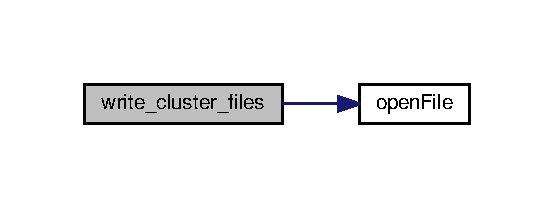
\includegraphics[width=266pt]{io_8c_a328704f75c999c31e485b3542a26207d_cgraph}
\end{center}
\end{figure}




Here is the caller graph for this function\-:\nopagebreak
\begin{figure}[H]
\begin{center}
\leavevmode
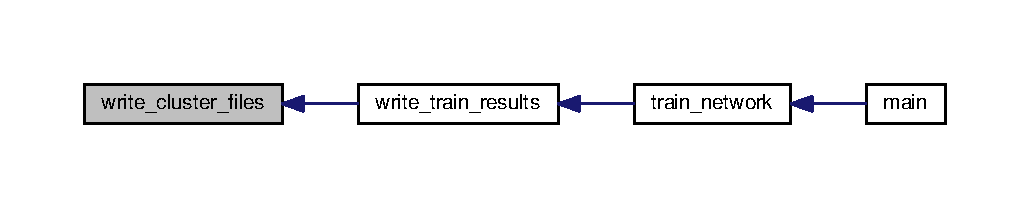
\includegraphics[width=350pt]{io_8c_a328704f75c999c31e485b3542a26207d_icgraph}
\end{center}
\end{figure}


\hypertarget{io_8c_afaadde76430f928670e1054153da6677}{\index{io.\-c@{io.\-c}!write\-\_\-clusts\-\_\-classes@{write\-\_\-clusts\-\_\-classes}}
\index{write\-\_\-clusts\-\_\-classes@{write\-\_\-clusts\-\_\-classes}!io.c@{io.\-c}}
\subsubsection[{write\-\_\-clusts\-\_\-classes}]{\setlength{\rightskip}{0pt plus 5cm}static void write\-\_\-clusts\-\_\-classes (
\begin{DoxyParamCaption}
\item[{Vector $\ast$$\ast$}]{clusts\-Class, }
\item[{F\-I\-L\-E $\ast$}]{out, }
\item[{Vector $\ast$}]{clusts, }
\item[{Vector $\ast$}]{pats\-Class}
\end{DoxyParamCaption}
)\hspace{0.3cm}{\ttfamily [static]}}}\label{io_8c_afaadde76430f928670e1054153da6677}
Write the number of patterns in each class, in each cluster.

For instance, in the mushrooms database there's two classes\-: p (poisonous) and e (edible). Then the repartition looks like\-: 
\begin{DoxyCode}
No. cluster |    p    |    e    | Class
------------+---------+---------+------
          0 |     274 |     320 | e
          1 |       0 |     768 | e
          2 |      32 |     108 | e
          3 |      72 |     443 | e
               [...]
         15 |       8 |       0 | p
         16 |       0 |      16 | e
\end{DoxyCode}
 The class column indicate the clusters's classes\-: the prominent class of the cluster.

This function would deserved a little clean up. It is a long function for a small job but it actually generate ascii tables for any number of classes of any lengths.


\begin{DoxyParams}[1]{Parameters}
\mbox{\tt out}  & {\em clusts\-Class} & The array that will be filled with the clusters's classes. \\
\hline
\mbox{\tt in}  & {\em out} & The output file where the classes repartition will be written. \\
\hline
\mbox{\tt in}  & {\em clusts} & The network clusters. \\
\hline
\mbox{\tt in}  & {\em pats\-Class} & The network training patterns classes. \\
\hline
\end{DoxyParams}


Here is the caller graph for this function\-:\nopagebreak
\begin{figure}[H]
\begin{center}
\leavevmode
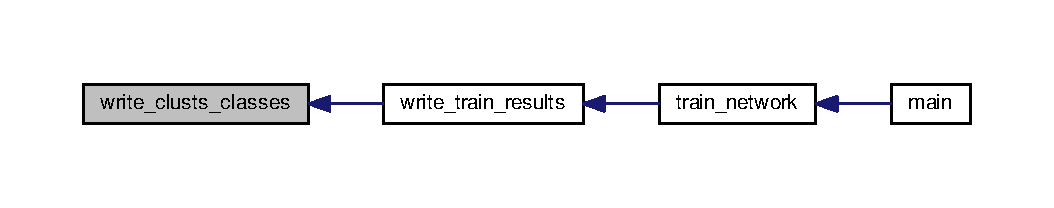
\includegraphics[width=350pt]{io_8c_afaadde76430f928670e1054153da6677_icgraph}
\end{center}
\end{figure}


\hypertarget{io_8c_a4e19be6f887c6b2c836348fce9ca5b0f}{\index{io.\-c@{io.\-c}!write\-\_\-clusts\-\_\-pat\-\_\-sets@{write\-\_\-clusts\-\_\-pat\-\_\-sets}}
\index{write\-\_\-clusts\-\_\-pat\-\_\-sets@{write\-\_\-clusts\-\_\-pat\-\_\-sets}!io.c@{io.\-c}}
\subsubsection[{write\-\_\-clusts\-\_\-pat\-\_\-sets}]{\setlength{\rightskip}{0pt plus 5cm}static void write\-\_\-clusts\-\_\-pat\-\_\-sets (
\begin{DoxyParamCaption}
\item[{F\-I\-L\-E $\ast$}]{out, }
\item[{Vector $\ast$}]{clusts}
\end{DoxyParamCaption}
)\hspace{0.3cm}{\ttfamily [static]}}}\label{io_8c_a4e19be6f887c6b2c836348fce9ca5b0f}


Here is the caller graph for this function\-:\nopagebreak
\begin{figure}[H]
\begin{center}
\leavevmode
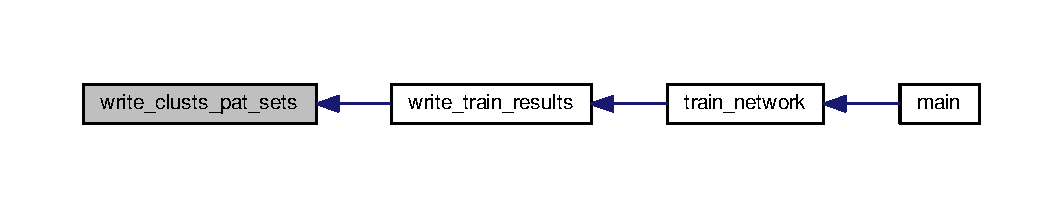
\includegraphics[width=350pt]{io_8c_a4e19be6f887c6b2c836348fce9ca5b0f_icgraph}
\end{center}
\end{figure}


\hypertarget{io_8c_ac238d5ff2b2ee59bdd90bed4188bb86a}{\index{io.\-c@{io.\-c}!write\-\_\-clusts\-\_\-prototypes@{write\-\_\-clusts\-\_\-prototypes}}
\index{write\-\_\-clusts\-\_\-prototypes@{write\-\_\-clusts\-\_\-prototypes}!io.c@{io.\-c}}
\subsubsection[{write\-\_\-clusts\-\_\-prototypes}]{\setlength{\rightskip}{0pt plus 5cm}static void write\-\_\-clusts\-\_\-prototypes (
\begin{DoxyParamCaption}
\item[{F\-I\-L\-E $\ast$}]{out, }
\item[{{\bf In\-Param}}]{par, }
\item[{Vector $\ast$}]{clusts, }
\item[{{\bf ulong}}]{n\-Clusts}
\end{DoxyParamCaption}
)\hspace{0.3cm}{\ttfamily [static]}}}\label{io_8c_ac238d5ff2b2ee59bdd90bed4188bb86a}
Write the prototype of every clusters in the given file.


\begin{DoxyParams}[1]{Parameters}
\mbox{\tt in}  & {\em out} & The output file where the prototypes will be written. \\
\hline
\mbox{\tt in}  & {\em par} & The network parameters. \\
\hline
\mbox{\tt in}  & {\em clusts} & The network clusters. \\
\hline
\mbox{\tt in}  & {\em n\-Clusts} & Number of network clusters. \\
\hline
\end{DoxyParams}


Here is the caller graph for this function\-:\nopagebreak
\begin{figure}[H]
\begin{center}
\leavevmode
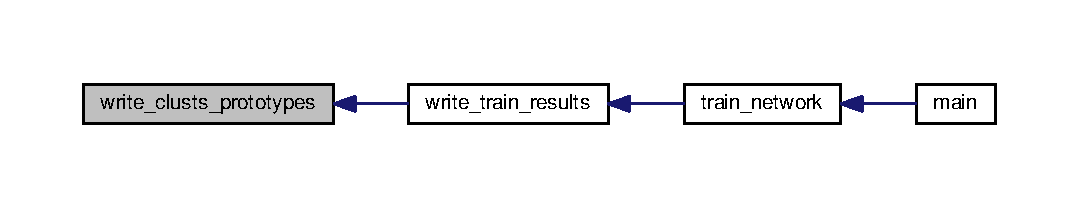
\includegraphics[width=350pt]{io_8c_ac238d5ff2b2ee59bdd90bed4188bb86a_icgraph}
\end{center}
\end{figure}


\hypertarget{io_8c_a965830f0ac8cd6fb565d8e7fd040c950}{\index{io.\-c@{io.\-c}!write\-\_\-ratio@{write\-\_\-ratio}}
\index{write\-\_\-ratio@{write\-\_\-ratio}!io.c@{io.\-c}}
\subsubsection[{write\-\_\-ratio}]{\setlength{\rightskip}{0pt plus 5cm}static void write\-\_\-ratio (
\begin{DoxyParamCaption}
\item[{F\-I\-L\-E $\ast$}]{out, }
\item[{Vector $\ast$}]{pats, }
\item[{Vector $\ast$}]{clusts, }
\item[{Vector $\ast$}]{pats\-Class, }
\item[{Vector $\ast$}]{clusts\-Class}
\end{DoxyParamCaption}
)\hspace{0.3cm}{\ttfamily [static]}}}\label{io_8c_a965830f0ac8cd6fb565d8e7fd040c950}
Write the success / fail ratio of the training stage in the given file.


\begin{DoxyParams}[1]{Parameters}
\mbox{\tt in}  & {\em out} & The output file where the prototypes will be written. \\
\hline
\mbox{\tt in}  & {\em pats} & The network training patterns set. \\
\hline
\mbox{\tt in}  & {\em clusts} & The network clusters. \\
\hline
\mbox{\tt in}  & {\em pats\-Class} & The network training patterns classes. \\
\hline
\mbox{\tt in}  & {\em clusts\-Class} & The network clusters classes. \\
\hline
\end{DoxyParams}


Here is the call graph for this function\-:\nopagebreak
\begin{figure}[H]
\begin{center}
\leavevmode
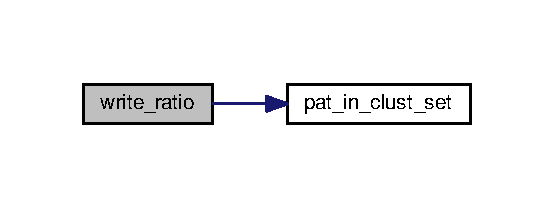
\includegraphics[width=266pt]{io_8c_a965830f0ac8cd6fb565d8e7fd040c950_cgraph}
\end{center}
\end{figure}




Here is the caller graph for this function\-:\nopagebreak
\begin{figure}[H]
\begin{center}
\leavevmode
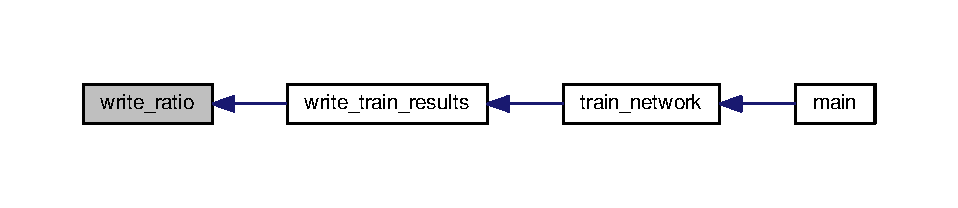
\includegraphics[width=350pt]{io_8c_a965830f0ac8cd6fb565d8e7fd040c950_icgraph}
\end{center}
\end{figure}


\hypertarget{io_8c_aa7db0c1a52daa6b67e37b56e9b48bdc3}{\index{io.\-c@{io.\-c}!write\-\_\-test\-\_\-results@{write\-\_\-test\-\_\-results}}
\index{write\-\_\-test\-\_\-results@{write\-\_\-test\-\_\-results}!io.c@{io.\-c}}
\subsubsection[{write\-\_\-test\-\_\-results}]{\setlength{\rightskip}{0pt plus 5cm}void write\-\_\-test\-\_\-results (
\begin{DoxyParamCaption}
\item[{{\bf In\-Param}}]{par, }
\item[{{\bf ulong}}]{empty\-Pats, }
\item[{Vector $\ast$}]{pats, }
\item[{{\bf ulong}}]{n\-Pats, }
\item[{Vector $\ast$}]{clusts, }
\item[{Vector $\ast$}]{test\-Classes, }
\item[{Vector $\ast$}]{test\-Res\-Classes}
\end{DoxyParamCaption}
)}}\label{io_8c_aa7db0c1a52daa6b67e37b56e9b48bdc3}


Here is the call graph for this function\-:\nopagebreak
\begin{figure}[H]
\begin{center}
\leavevmode
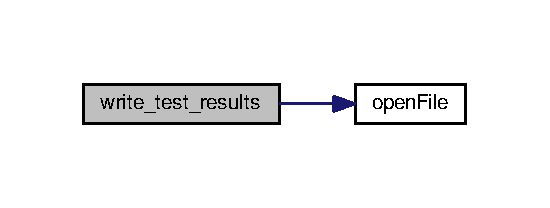
\includegraphics[width=264pt]{io_8c_aa7db0c1a52daa6b67e37b56e9b48bdc3_cgraph}
\end{center}
\end{figure}




Here is the caller graph for this function\-:\nopagebreak
\begin{figure}[H]
\begin{center}
\leavevmode
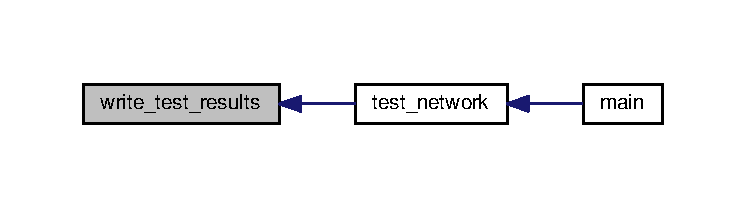
\includegraphics[width=350pt]{io_8c_aa7db0c1a52daa6b67e37b56e9b48bdc3_icgraph}
\end{center}
\end{figure}


\hypertarget{io_8c_a72d8ceea6208425220d76bc1d02b7498}{\index{io.\-c@{io.\-c}!write\-\_\-train\-\_\-results@{write\-\_\-train\-\_\-results}}
\index{write\-\_\-train\-\_\-results@{write\-\_\-train\-\_\-results}!io.c@{io.\-c}}
\subsubsection[{write\-\_\-train\-\_\-results}]{\setlength{\rightskip}{0pt plus 5cm}void write\-\_\-train\-\_\-results (
\begin{DoxyParamCaption}
\item[{Vector $\ast$$\ast$}]{clusts\-Classes, }
\item[{{\bf In\-Param}}]{par, }
\item[{{\bf ulong}}]{empty\-Pats, }
\item[{float}]{fluc, }
\item[{Vector $\ast$}]{pats, }
\item[{{\bf ulong}}]{n\-Pats, }
\item[{Vector $\ast$}]{clusts, }
\item[{Vector $\ast$}]{pats\-Class}
\end{DoxyParamCaption}
)}}\label{io_8c_a72d8ceea6208425220d76bc1d02b7498}
Write the result datas on the output files.

There's too much datas to write them on the terminal so they are written on output files. The main output file is \char`\"{}art\-\_\-results\char`\"{} (by default) and it contains every information used to build and train the network. Other output files are named \char`\"{}art\-\_\-clust\-\_\-xxx.\-csv\char`\"{} and they contains the cluster \#xxx prototype followed by every patterns which belongs to this cluster.

\begin{DoxyRefDesc}{Todo}
\item[\hyperlink{todo__todo000003}{Todo}]It would be a good idea to use the output file in order to load a network.\end{DoxyRefDesc}



\begin{DoxyParams}[1]{Parameters}
\mbox{\tt out}  & {\em clusts\-Class} & The array that will be filled with the clusters's classes. \\
\hline
\mbox{\tt in}  & {\em par} & The network parameters. \\
\hline
\mbox{\tt in}  & {\em empty\-Pats} & Number of empty patterns removed. \\
\hline
\mbox{\tt in}  & {\em fluc} & The best recorded fluctuation. \\
\hline
\mbox{\tt in}  & {\em pats} & The network training patterns set. \\
\hline
\mbox{\tt in}  & {\em n\-Pats} & Number of training patterns of the network. \\
\hline
\mbox{\tt in}  & {\em clusts} & The network clusters. \\
\hline
\mbox{\tt in}  & {\em pats\-Class} & The network training patterns classes. \\
\hline
\end{DoxyParams}


Here is the call graph for this function\-:\nopagebreak
\begin{figure}[H]
\begin{center}
\leavevmode
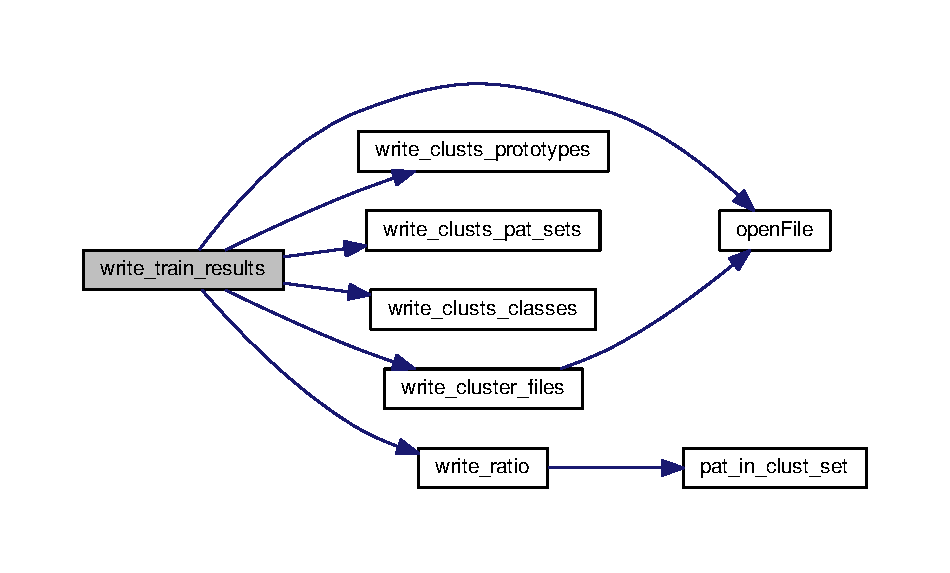
\includegraphics[width=350pt]{io_8c_a72d8ceea6208425220d76bc1d02b7498_cgraph}
\end{center}
\end{figure}




Here is the caller graph for this function\-:\nopagebreak
\begin{figure}[H]
\begin{center}
\leavevmode
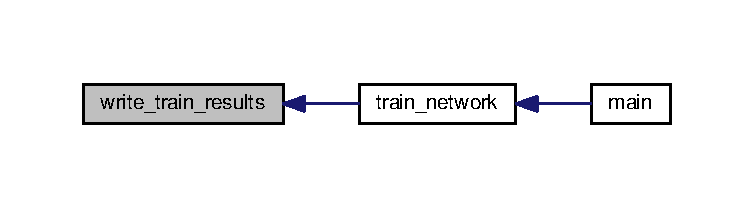
\includegraphics[width=350pt]{io_8c_a72d8ceea6208425220d76bc1d02b7498_icgraph}
\end{center}
\end{figure}



\hypertarget{io_8h}{\section{src/io.h File Reference}
\label{io_8h}\index{src/io.\-h@{src/io.\-h}}
}
{\ttfamily \#include $<$stdio.\-h$>$}\\*
{\ttfamily \#include \char`\"{}utls.\-h\char`\"{}}\\*
Include dependency graph for io.\-h\-:\nopagebreak
\begin{figure}[H]
\begin{center}
\leavevmode
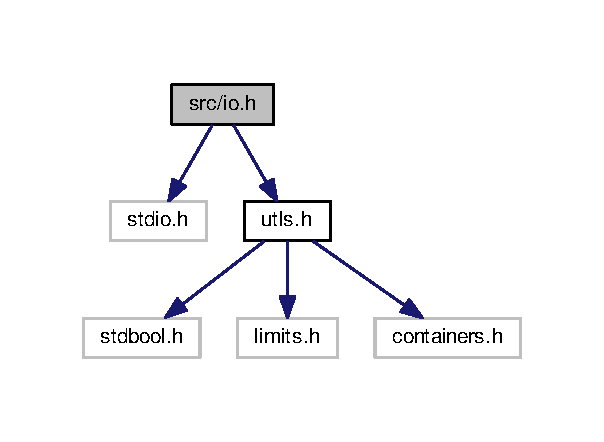
\includegraphics[width=290pt]{io_8h__incl}
\end{center}
\end{figure}
This graph shows which files directly or indirectly include this file\-:\nopagebreak
\begin{figure}[H]
\begin{center}
\leavevmode
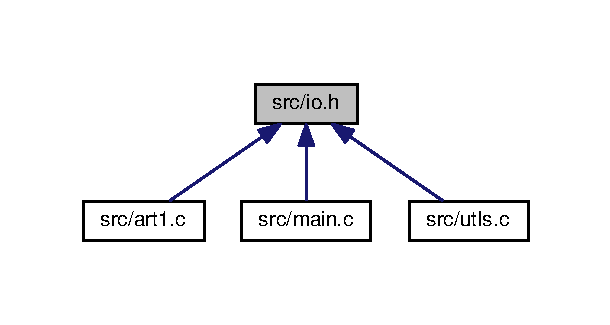
\includegraphics[width=293pt]{io_8h__dep__incl}
\end{center}
\end{figure}
\subsection*{Macros}
\begin{DoxyCompactItemize}
\item 
\#define \hyperlink{io_8h_a980a5417a58b32be68d8063dda364a04}{R\-E\-S\-\_\-\-S\-U\-F\-F\-I\-X}~\char`\"{}\-\_\-results\char`\"{}
\item 
\#define \hyperlink{io_8h_ac2af17fb59e4dd72455a2a99c1ca6716}{C\-L\-U\-S\-T\-\_\-\-S\-U\-F\-F\-I\-X}~\char`\"{}\-\_\-clust\char`\"{}
\item 
\#define \hyperlink{io_8h_adaf830ca173e11fc53174cfc3250ef3e}{R\-E\-S\-\_\-\-F\-O\-L\-D\-E\-R}~\char`\"{}./results/\char`\"{}
\item 
\#define \hyperlink{io_8h_af1520efb1b81efc199e3b4b488c60e86}{C\-L\-U\-S\-T\-\_\-\-F\-O\-L\-D\-E\-R}~\char`\"{}clusters/\char`\"{}
\item 
\#define \hyperlink{io_8h_a4a33efa30320c5b77b9bcbeaab6b1dad}{T\-R\-A\-I\-N\-\_\-\-F\-O\-L\-D\-E\-R}~\char`\"{}train/\char`\"{}
\item 
\#define \hyperlink{io_8h_a56f1bb9c70e7f125dbc93addc313c6fc}{T\-E\-S\-T\-\_\-\-F\-O\-L\-D\-E\-R}~\char`\"{}test/\char`\"{}
\end{DoxyCompactItemize}
\subsection*{Functions}
\begin{DoxyCompactItemize}
\item 
void \hyperlink{io_8h_a80f8a74945aebf5dcfdeab96825d5f1c}{set\-\_\-network\-\_\-values} (\hyperlink{struct_in_param}{In\-Param} $\ast$par, int argc, const char $\ast$argv\mbox{[}$\,$\mbox{]})
\item 
void \hyperlink{io_8h_ae358f42d763b99428cdf3e715bbc796f}{print\-\_\-network\-\_\-values} (\hyperlink{struct_in_param}{In\-Param} par)
\item 
void \hyperlink{io_8h_ad8b111857701d408852c427d3a6e4506}{vec\-\_\-print\-\_\-char\-\_\-as\-\_\-int} (Vector $\ast$vec)
\item 
void \hyperlink{io_8h_af6b21dcee544a6af4211e0471ef2a64b}{vec\-\_\-print\-\_\-as\-\_\-char} (Vector $\ast$vec)
\item 
void \hyperlink{io_8h_a28bccc0516042023b1f6e9d06fd531c0}{vector\-\_\-print\-\_\-ulong} (Vector $\ast$vec)
\item 
int \hyperlink{io_8h_a3405b5370d2c756dc5135a5bf8fbdc34}{open\-File} (F\-I\-L\-E $\ast$$\ast$file, const char $\ast$name, char const $\ast$mode)
\item 
void \hyperlink{io_8h_ad3f3f9a2e30a9158c82206fb913f2b3d}{read\-Csv} (\hyperlink{utls_8h_a718b4eb2652c286f4d42dc18a8e71a1a}{ulong} $\ast$plen, List $\ast$lines, F\-I\-L\-E $\ast$file, bool skip)
\item 
void \hyperlink{io_8h_a72d8ceea6208425220d76bc1d02b7498}{write\-\_\-train\-\_\-results} (Vector $\ast$$\ast$clusts\-Classes, \hyperlink{struct_in_param}{In\-Param} par, \hyperlink{utls_8h_a718b4eb2652c286f4d42dc18a8e71a1a}{ulong} empty\-Pats, float fluc, Vector $\ast$pats, \hyperlink{utls_8h_a718b4eb2652c286f4d42dc18a8e71a1a}{ulong} n\-Pats, Vector $\ast$clusts, Vector $\ast$pats\-Class)
\item 
void \hyperlink{io_8h_afccc516ea32de34dd430ad12c045d15f}{write\-\_\-test\-\_\-results} (\hyperlink{struct_in_param}{In\-Param} par, \hyperlink{utls_8h_a718b4eb2652c286f4d42dc18a8e71a1a}{ulong} empty\-Pats, Vector $\ast$pats, \hyperlink{utls_8h_a718b4eb2652c286f4d42dc18a8e71a1a}{ulong} n\-Pats, Vector $\ast$clusts, Vector $\ast$pats\-Class, Vector $\ast$test\-Res\-Classes)
\end{DoxyCompactItemize}


\subsection{Macro Definition Documentation}
\hypertarget{io_8h_af1520efb1b81efc199e3b4b488c60e86}{\index{io.\-h@{io.\-h}!C\-L\-U\-S\-T\-\_\-\-F\-O\-L\-D\-E\-R@{C\-L\-U\-S\-T\-\_\-\-F\-O\-L\-D\-E\-R}}
\index{C\-L\-U\-S\-T\-\_\-\-F\-O\-L\-D\-E\-R@{C\-L\-U\-S\-T\-\_\-\-F\-O\-L\-D\-E\-R}!io.h@{io.\-h}}
\subsubsection[{C\-L\-U\-S\-T\-\_\-\-F\-O\-L\-D\-E\-R}]{\setlength{\rightskip}{0pt plus 5cm}\#define C\-L\-U\-S\-T\-\_\-\-F\-O\-L\-D\-E\-R~\char`\"{}clusters/\char`\"{}}}\label{io_8h_af1520efb1b81efc199e3b4b488c60e86}
\hypertarget{io_8h_ac2af17fb59e4dd72455a2a99c1ca6716}{\index{io.\-h@{io.\-h}!C\-L\-U\-S\-T\-\_\-\-S\-U\-F\-F\-I\-X@{C\-L\-U\-S\-T\-\_\-\-S\-U\-F\-F\-I\-X}}
\index{C\-L\-U\-S\-T\-\_\-\-S\-U\-F\-F\-I\-X@{C\-L\-U\-S\-T\-\_\-\-S\-U\-F\-F\-I\-X}!io.h@{io.\-h}}
\subsubsection[{C\-L\-U\-S\-T\-\_\-\-S\-U\-F\-F\-I\-X}]{\setlength{\rightskip}{0pt plus 5cm}\#define C\-L\-U\-S\-T\-\_\-\-S\-U\-F\-F\-I\-X~\char`\"{}\-\_\-clust\char`\"{}}}\label{io_8h_ac2af17fb59e4dd72455a2a99c1ca6716}
\hypertarget{io_8h_adaf830ca173e11fc53174cfc3250ef3e}{\index{io.\-h@{io.\-h}!R\-E\-S\-\_\-\-F\-O\-L\-D\-E\-R@{R\-E\-S\-\_\-\-F\-O\-L\-D\-E\-R}}
\index{R\-E\-S\-\_\-\-F\-O\-L\-D\-E\-R@{R\-E\-S\-\_\-\-F\-O\-L\-D\-E\-R}!io.h@{io.\-h}}
\subsubsection[{R\-E\-S\-\_\-\-F\-O\-L\-D\-E\-R}]{\setlength{\rightskip}{0pt plus 5cm}\#define R\-E\-S\-\_\-\-F\-O\-L\-D\-E\-R~\char`\"{}./results/\char`\"{}}}\label{io_8h_adaf830ca173e11fc53174cfc3250ef3e}
\hypertarget{io_8h_a980a5417a58b32be68d8063dda364a04}{\index{io.\-h@{io.\-h}!R\-E\-S\-\_\-\-S\-U\-F\-F\-I\-X@{R\-E\-S\-\_\-\-S\-U\-F\-F\-I\-X}}
\index{R\-E\-S\-\_\-\-S\-U\-F\-F\-I\-X@{R\-E\-S\-\_\-\-S\-U\-F\-F\-I\-X}!io.h@{io.\-h}}
\subsubsection[{R\-E\-S\-\_\-\-S\-U\-F\-F\-I\-X}]{\setlength{\rightskip}{0pt plus 5cm}\#define R\-E\-S\-\_\-\-S\-U\-F\-F\-I\-X~\char`\"{}\-\_\-results\char`\"{}}}\label{io_8h_a980a5417a58b32be68d8063dda364a04}
\hypertarget{io_8h_a56f1bb9c70e7f125dbc93addc313c6fc}{\index{io.\-h@{io.\-h}!T\-E\-S\-T\-\_\-\-F\-O\-L\-D\-E\-R@{T\-E\-S\-T\-\_\-\-F\-O\-L\-D\-E\-R}}
\index{T\-E\-S\-T\-\_\-\-F\-O\-L\-D\-E\-R@{T\-E\-S\-T\-\_\-\-F\-O\-L\-D\-E\-R}!io.h@{io.\-h}}
\subsubsection[{T\-E\-S\-T\-\_\-\-F\-O\-L\-D\-E\-R}]{\setlength{\rightskip}{0pt plus 5cm}\#define T\-E\-S\-T\-\_\-\-F\-O\-L\-D\-E\-R~\char`\"{}test/\char`\"{}}}\label{io_8h_a56f1bb9c70e7f125dbc93addc313c6fc}
\hypertarget{io_8h_a4a33efa30320c5b77b9bcbeaab6b1dad}{\index{io.\-h@{io.\-h}!T\-R\-A\-I\-N\-\_\-\-F\-O\-L\-D\-E\-R@{T\-R\-A\-I\-N\-\_\-\-F\-O\-L\-D\-E\-R}}
\index{T\-R\-A\-I\-N\-\_\-\-F\-O\-L\-D\-E\-R@{T\-R\-A\-I\-N\-\_\-\-F\-O\-L\-D\-E\-R}!io.h@{io.\-h}}
\subsubsection[{T\-R\-A\-I\-N\-\_\-\-F\-O\-L\-D\-E\-R}]{\setlength{\rightskip}{0pt plus 5cm}\#define T\-R\-A\-I\-N\-\_\-\-F\-O\-L\-D\-E\-R~\char`\"{}train/\char`\"{}}}\label{io_8h_a4a33efa30320c5b77b9bcbeaab6b1dad}


\subsection{Function Documentation}
\hypertarget{io_8h_a3405b5370d2c756dc5135a5bf8fbdc34}{\index{io.\-h@{io.\-h}!open\-File@{open\-File}}
\index{open\-File@{open\-File}!io.h@{io.\-h}}
\subsubsection[{open\-File}]{\setlength{\rightskip}{0pt plus 5cm}int open\-File (
\begin{DoxyParamCaption}
\item[{F\-I\-L\-E $\ast$$\ast$}]{file, }
\item[{const char $\ast$}]{name, }
\item[{char const $\ast$}]{mode}
\end{DoxyParamCaption}
)}}\label{io_8h_a3405b5370d2c756dc5135a5bf8fbdc34}


Here is the caller graph for this function\-:\nopagebreak
\begin{figure}[H]
\begin{center}
\leavevmode
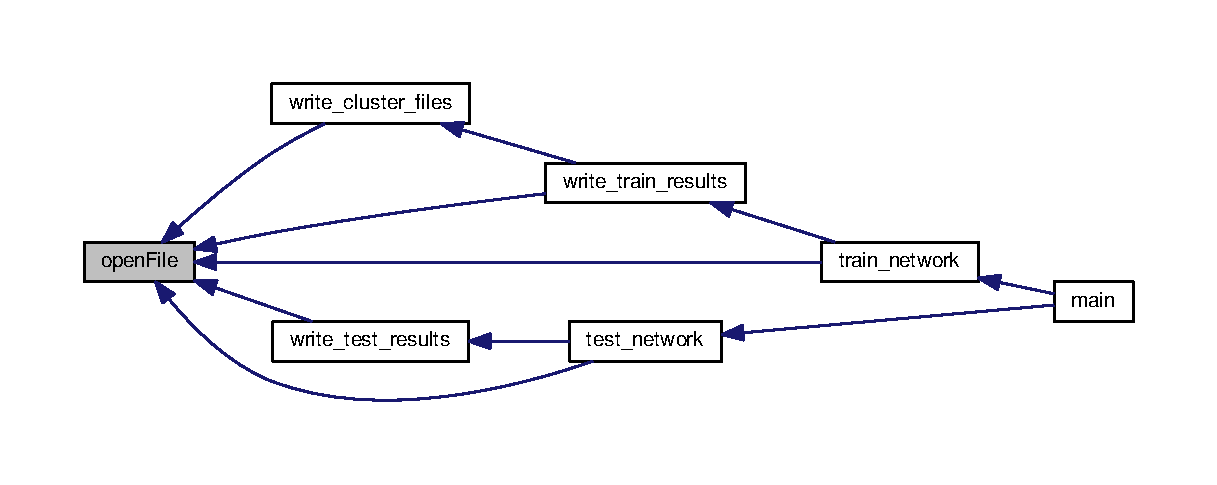
\includegraphics[width=350pt]{io_8h_a3405b5370d2c756dc5135a5bf8fbdc34_icgraph}
\end{center}
\end{figure}


\hypertarget{io_8h_ae358f42d763b99428cdf3e715bbc796f}{\index{io.\-h@{io.\-h}!print\-\_\-network\-\_\-values@{print\-\_\-network\-\_\-values}}
\index{print\-\_\-network\-\_\-values@{print\-\_\-network\-\_\-values}!io.h@{io.\-h}}
\subsubsection[{print\-\_\-network\-\_\-values}]{\setlength{\rightskip}{0pt plus 5cm}void print\-\_\-network\-\_\-values (
\begin{DoxyParamCaption}
\item[{{\bf In\-Param}}]{par}
\end{DoxyParamCaption}
)}}\label{io_8h_ae358f42d763b99428cdf3e715bbc796f}


Here is the caller graph for this function\-:\nopagebreak
\begin{figure}[H]
\begin{center}
\leavevmode
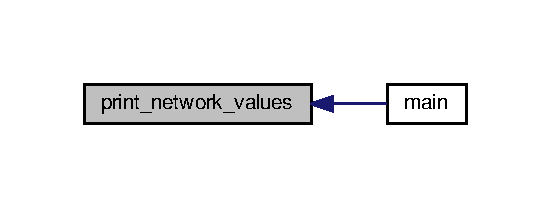
\includegraphics[width=264pt]{io_8h_ae358f42d763b99428cdf3e715bbc796f_icgraph}
\end{center}
\end{figure}


\hypertarget{io_8h_ad3f3f9a2e30a9158c82206fb913f2b3d}{\index{io.\-h@{io.\-h}!read\-Csv@{read\-Csv}}
\index{read\-Csv@{read\-Csv}!io.h@{io.\-h}}
\subsubsection[{read\-Csv}]{\setlength{\rightskip}{0pt plus 5cm}void read\-Csv (
\begin{DoxyParamCaption}
\item[{{\bf ulong} $\ast$}]{plen, }
\item[{List $\ast$}]{lines, }
\item[{F\-I\-L\-E $\ast$}]{file, }
\item[{bool}]{skip}
\end{DoxyParamCaption}
)}}\label{io_8h_ad3f3f9a2e30a9158c82206fb913f2b3d}


Here is the caller graph for this function\-:\nopagebreak
\begin{figure}[H]
\begin{center}
\leavevmode
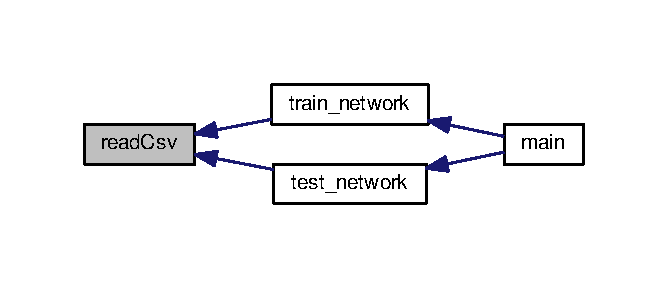
\includegraphics[width=320pt]{io_8h_ad3f3f9a2e30a9158c82206fb913f2b3d_icgraph}
\end{center}
\end{figure}


\hypertarget{io_8h_a80f8a74945aebf5dcfdeab96825d5f1c}{\index{io.\-h@{io.\-h}!set\-\_\-network\-\_\-values@{set\-\_\-network\-\_\-values}}
\index{set\-\_\-network\-\_\-values@{set\-\_\-network\-\_\-values}!io.h@{io.\-h}}
\subsubsection[{set\-\_\-network\-\_\-values}]{\setlength{\rightskip}{0pt plus 5cm}void set\-\_\-network\-\_\-values (
\begin{DoxyParamCaption}
\item[{{\bf In\-Param} $\ast$}]{par, }
\item[{int}]{argc, }
\item[{const char $\ast$}]{argv\mbox{[}$\,$\mbox{]}}
\end{DoxyParamCaption}
)}}\label{io_8h_a80f8a74945aebf5dcfdeab96825d5f1c}


Here is the caller graph for this function\-:\nopagebreak
\begin{figure}[H]
\begin{center}
\leavevmode
\includegraphics[width=258pt]{io_8h_a80f8a74945aebf5dcfdeab96825d5f1c_icgraph}
\end{center}
\end{figure}


\hypertarget{io_8h_af6b21dcee544a6af4211e0471ef2a64b}{\index{io.\-h@{io.\-h}!vec\-\_\-print\-\_\-as\-\_\-char@{vec\-\_\-print\-\_\-as\-\_\-char}}
\index{vec\-\_\-print\-\_\-as\-\_\-char@{vec\-\_\-print\-\_\-as\-\_\-char}!io.h@{io.\-h}}
\subsubsection[{vec\-\_\-print\-\_\-as\-\_\-char}]{\setlength{\rightskip}{0pt plus 5cm}void vec\-\_\-print\-\_\-as\-\_\-char (
\begin{DoxyParamCaption}
\item[{Vector $\ast$}]{vec}
\end{DoxyParamCaption}
)}}\label{io_8h_af6b21dcee544a6af4211e0471ef2a64b}
\hypertarget{io_8h_ad8b111857701d408852c427d3a6e4506}{\index{io.\-h@{io.\-h}!vec\-\_\-print\-\_\-char\-\_\-as\-\_\-int@{vec\-\_\-print\-\_\-char\-\_\-as\-\_\-int}}
\index{vec\-\_\-print\-\_\-char\-\_\-as\-\_\-int@{vec\-\_\-print\-\_\-char\-\_\-as\-\_\-int}!io.h@{io.\-h}}
\subsubsection[{vec\-\_\-print\-\_\-char\-\_\-as\-\_\-int}]{\setlength{\rightskip}{0pt plus 5cm}void vec\-\_\-print\-\_\-char\-\_\-as\-\_\-int (
\begin{DoxyParamCaption}
\item[{Vector $\ast$}]{vec}
\end{DoxyParamCaption}
)}}\label{io_8h_ad8b111857701d408852c427d3a6e4506}
\hypertarget{io_8h_a28bccc0516042023b1f6e9d06fd531c0}{\index{io.\-h@{io.\-h}!vector\-\_\-print\-\_\-ulong@{vector\-\_\-print\-\_\-ulong}}
\index{vector\-\_\-print\-\_\-ulong@{vector\-\_\-print\-\_\-ulong}!io.h@{io.\-h}}
\subsubsection[{vector\-\_\-print\-\_\-ulong}]{\setlength{\rightskip}{0pt plus 5cm}void vector\-\_\-print\-\_\-ulong (
\begin{DoxyParamCaption}
\item[{Vector $\ast$}]{vec}
\end{DoxyParamCaption}
)}}\label{io_8h_a28bccc0516042023b1f6e9d06fd531c0}
\hypertarget{io_8h_afccc516ea32de34dd430ad12c045d15f}{\index{io.\-h@{io.\-h}!write\-\_\-test\-\_\-results@{write\-\_\-test\-\_\-results}}
\index{write\-\_\-test\-\_\-results@{write\-\_\-test\-\_\-results}!io.h@{io.\-h}}
\subsubsection[{write\-\_\-test\-\_\-results}]{\setlength{\rightskip}{0pt plus 5cm}void write\-\_\-test\-\_\-results (
\begin{DoxyParamCaption}
\item[{{\bf In\-Param}}]{par, }
\item[{{\bf ulong}}]{empty\-Pats, }
\item[{Vector $\ast$}]{pats, }
\item[{{\bf ulong}}]{n\-Pats, }
\item[{Vector $\ast$}]{clusts, }
\item[{Vector $\ast$}]{pats\-Class, }
\item[{Vector $\ast$}]{test\-Res\-Classes}
\end{DoxyParamCaption}
)}}\label{io_8h_afccc516ea32de34dd430ad12c045d15f}


Here is the call graph for this function\-:\nopagebreak
\begin{figure}[H]
\begin{center}
\leavevmode
\includegraphics[width=264pt]{io_8h_afccc516ea32de34dd430ad12c045d15f_cgraph}
\end{center}
\end{figure}




Here is the caller graph for this function\-:\nopagebreak
\begin{figure}[H]
\begin{center}
\leavevmode
\includegraphics[width=350pt]{io_8h_afccc516ea32de34dd430ad12c045d15f_icgraph}
\end{center}
\end{figure}


\hypertarget{io_8h_a72d8ceea6208425220d76bc1d02b7498}{\index{io.\-h@{io.\-h}!write\-\_\-train\-\_\-results@{write\-\_\-train\-\_\-results}}
\index{write\-\_\-train\-\_\-results@{write\-\_\-train\-\_\-results}!io.h@{io.\-h}}
\subsubsection[{write\-\_\-train\-\_\-results}]{\setlength{\rightskip}{0pt plus 5cm}void write\-\_\-train\-\_\-results (
\begin{DoxyParamCaption}
\item[{Vector $\ast$$\ast$}]{clusts\-Classes, }
\item[{{\bf In\-Param}}]{par, }
\item[{{\bf ulong}}]{empty\-Pats, }
\item[{float}]{fluc, }
\item[{Vector $\ast$}]{pats, }
\item[{{\bf ulong}}]{n\-Pats, }
\item[{Vector $\ast$}]{clusts, }
\item[{Vector $\ast$}]{pats\-Class}
\end{DoxyParamCaption}
)}}\label{io_8h_a72d8ceea6208425220d76bc1d02b7498}
Write the result datas on the output files.

There's too much datas to write them on the terminal so they are written on output files. The main output file is \char`\"{}art\-\_\-results\char`\"{} (by default) and it contains every information used to build and train the network. Other output files are named \char`\"{}art\-\_\-clust\-\_\-xxx.\-csv\char`\"{} and they contains the cluster \#xxx prototype followed by every patterns which belongs to this cluster.

\begin{DoxyRefDesc}{Todo}
\item[\hyperlink{todo__todo000003}{Todo}]It would be a good idea to use the output file in order to load a network.\end{DoxyRefDesc}



\begin{DoxyParams}[1]{Parameters}
\mbox{\tt out}  & {\em clusts\-Class} & The array that will be filled with the clusters's classes. \\
\hline
\mbox{\tt in}  & {\em par} & The network parameters. \\
\hline
\mbox{\tt in}  & {\em empty\-Pats} & Number of empty patterns removed. \\
\hline
\mbox{\tt in}  & {\em fluc} & The best recorded fluctuation. \\
\hline
\mbox{\tt in}  & {\em pats} & The network training patterns set. \\
\hline
\mbox{\tt in}  & {\em n\-Pats} & Number of training patterns of the network. \\
\hline
\mbox{\tt in}  & {\em clusts} & The network clusters. \\
\hline
\mbox{\tt in}  & {\em pats\-Class} & The network training patterns classes. \\
\hline
\end{DoxyParams}


Here is the call graph for this function\-:\nopagebreak
\begin{figure}[H]
\begin{center}
\leavevmode
\includegraphics[width=350pt]{io_8h_a72d8ceea6208425220d76bc1d02b7498_cgraph}
\end{center}
\end{figure}




Here is the caller graph for this function\-:\nopagebreak
\begin{figure}[H]
\begin{center}
\leavevmode
\includegraphics[width=350pt]{io_8h_a72d8ceea6208425220d76bc1d02b7498_icgraph}
\end{center}
\end{figure}



\hypertarget{main_8c}{\section{src/main.c File Reference}
\label{main_8c}\index{src/main.\-c@{src/main.\-c}}
}
{\ttfamily \#include $<$math.\-h$>$}\\*
{\ttfamily \#include $<$time.\-h$>$}\\*
{\ttfamily \#include \char`\"{}io.\-h\char`\"{}}\\*
{\ttfamily \#include \char`\"{}utls.\-h\char`\"{}}\\*
{\ttfamily \#include \char`\"{}art1.\-h\char`\"{}}\\*
{\ttfamily \#include \char`\"{}ccl\-\_\-internal.\-h\char`\"{}}\\*
Include dependency graph for main.\-c\-:\nopagebreak
\begin{figure}[H]
\begin{center}
\leavevmode
\includegraphics[width=350pt]{main_8c__incl}
\end{center}
\end{figure}
\subsection*{Functions}
\begin{DoxyCompactItemize}
\item 
static \hyperlink{utls_8h_a718b4eb2652c286f4d42dc18a8e71a1a}{ulong} \hyperlink{main_8c_ad047ee2c5ce4159e1cc2c5beeda083a8}{rm\-\_\-empty\-\_\-pats} (List $\ast$lines)
\item 
static \hyperlink{utls_8h_a718b4eb2652c286f4d42dc18a8e71a1a}{ulong} \hyperlink{main_8c_a4543a55853c336fe059621cc398361db}{check\-\_\-pats\-\_\-validity} (List $\ast$lines)
\item 
static void \hyperlink{main_8c_a1edc6738eab5530da319b2d8eaac3553}{add\-\_\-noise} (Vector $\ast$pats, int perc)
\item 
static void \hyperlink{main_8c_ab8a60154a65c7382a3eea6caf2badeca}{check\-\_\-binary} (List $\ast$lines, bool skip)
\item 
static void \hyperlink{main_8c_aed57d793bb4e50acb328306d4a46c15a}{train\-\_\-network} (\hyperlink{utls_8h_a718b4eb2652c286f4d42dc18a8e71a1a}{ulong} $\ast$pat\-Len, Vector $\ast$$\ast$best\-Clusts, Vector $\ast$$\ast$clusts\-Classes, \hyperlink{struct_in_param}{In\-Param} par)
\item 
static void \hyperlink{main_8c_a679215a5eaffbf7f0bc2bbbf4c3610f9}{test\-\_\-network} (\hyperlink{utls_8h_a718b4eb2652c286f4d42dc18a8e71a1a}{ulong} train\-Pat\-Len, Vector $\ast$clusts, Vector $\ast$clusts\-Classes, \hyperlink{struct_in_param}{In\-Param} par)
\item 
int \hyperlink{main_8c_ac0f2228420376f4db7e1274f2b41667c}{main} (int argc, const char $\ast$argv\mbox{[}$\,$\mbox{]})
\end{DoxyCompactItemize}


\subsection{Detailed Description}
\begin{DoxyAuthor}{Author}
Mathieu Fourcroy 
\end{DoxyAuthor}
\begin{DoxyDate}{Date}
June 2015 
\end{DoxyDate}
\begin{DoxyVersion}{Version}
0.\-0.\-1
\end{DoxyVersion}
\begin{DoxyRefDesc}{Todo}
\item[\hyperlink{todo__todo000004}{Todo}]Change the data structures to make it more readable. \end{DoxyRefDesc}


\subsection{Function Documentation}
\hypertarget{main_8c_a1edc6738eab5530da319b2d8eaac3553}{\index{main.\-c@{main.\-c}!add\-\_\-noise@{add\-\_\-noise}}
\index{add\-\_\-noise@{add\-\_\-noise}!main.c@{main.\-c}}
\subsubsection[{add\-\_\-noise}]{\setlength{\rightskip}{0pt plus 5cm}static void add\-\_\-noise (
\begin{DoxyParamCaption}
\item[{Vector $\ast$}]{pats, }
\item[{int}]{perc}
\end{DoxyParamCaption}
)\hspace{0.3cm}{\ttfamily [static]}}}\label{main_8c_a1edc6738eab5530da319b2d8eaac3553}
Add noise to each patterns of the patterns vector.

The noise is added by flipping random bits of the patterns.


\begin{DoxyParams}[1]{Parameters}
\mbox{\tt in,out}  & {\em pats} & The patterns which will be \char`\"{}noised\char`\"{}. \\
\hline
\mbox{\tt in}  & {\em perc} & The noise percentage to add to the patterns. \\
\hline
\end{DoxyParams}


Here is the caller graph for this function\-:\nopagebreak
\begin{figure}[H]
\begin{center}
\leavevmode
\includegraphics[width=328pt]{main_8c_a1edc6738eab5530da319b2d8eaac3553_icgraph}
\end{center}
\end{figure}


\hypertarget{main_8c_ab8a60154a65c7382a3eea6caf2badeca}{\index{main.\-c@{main.\-c}!check\-\_\-binary@{check\-\_\-binary}}
\index{check\-\_\-binary@{check\-\_\-binary}!main.c@{main.\-c}}
\subsubsection[{check\-\_\-binary}]{\setlength{\rightskip}{0pt plus 5cm}static void check\-\_\-binary (
\begin{DoxyParamCaption}
\item[{List $\ast$}]{lines, }
\item[{bool}]{skip}
\end{DoxyParamCaption}
)\hspace{0.3cm}{\ttfamily [static]}}}\label{main_8c_ab8a60154a65c7382a3eea6caf2badeca}
Check weither every patterns are maid of binary numbers (0/1).

The function dosen't return any boolean because it automaticaly exit the program if the patterns aren't binary\-: it's impossible to build an A\-R\-T1 network with non-\/binary patterns.


\begin{DoxyParams}[1]{Parameters}
\mbox{\tt in}  & {\em lines} & The list of patterns to check. \\
\hline
\mbox{\tt in}  & {\em skip} & Indicate weither the first attribute of the csv string must be skipped or not. \\
\hline
\end{DoxyParams}


Here is the caller graph for this function\-:\nopagebreak
\begin{figure}[H]
\begin{center}
\leavevmode
\includegraphics[width=340pt]{main_8c_ab8a60154a65c7382a3eea6caf2badeca_icgraph}
\end{center}
\end{figure}


\hypertarget{main_8c_a4543a55853c336fe059621cc398361db}{\index{main.\-c@{main.\-c}!check\-\_\-pats\-\_\-validity@{check\-\_\-pats\-\_\-validity}}
\index{check\-\_\-pats\-\_\-validity@{check\-\_\-pats\-\_\-validity}!main.c@{main.\-c}}
\subsubsection[{check\-\_\-pats\-\_\-validity}]{\setlength{\rightskip}{0pt plus 5cm}static {\bf ulong} check\-\_\-pats\-\_\-validity (
\begin{DoxyParamCaption}
\item[{List $\ast$}]{lines}
\end{DoxyParamCaption}
)\hspace{0.3cm}{\ttfamily [static]}}}\label{main_8c_a4543a55853c336fe059621cc398361db}
Check the patterns validity.

Check\-:
\begin{DoxyItemize}
\item if there's enough patterns in the patterns list (at least 2).
\item if patterns aren't 0000000... (in that case\-: remove them).
\end{DoxyItemize}


\begin{DoxyParams}[1]{Parameters}
\mbox{\tt in}  & {\em lines} & The patterns list to check.\\
\hline
\end{DoxyParams}
\begin{DoxyReturn}{Returns}
The number of empty patterns removed. 
\end{DoxyReturn}


Here is the call graph for this function\-:\nopagebreak
\begin{figure}[H]
\begin{center}
\leavevmode
\includegraphics[width=304pt]{main_8c_a4543a55853c336fe059621cc398361db_cgraph}
\end{center}
\end{figure}




Here is the caller graph for this function\-:\nopagebreak
\begin{figure}[H]
\begin{center}
\leavevmode
\includegraphics[width=350pt]{main_8c_a4543a55853c336fe059621cc398361db_icgraph}
\end{center}
\end{figure}


\hypertarget{main_8c_ac0f2228420376f4db7e1274f2b41667c}{\index{main.\-c@{main.\-c}!main@{main}}
\index{main@{main}!main.c@{main.\-c}}
\subsubsection[{main}]{\setlength{\rightskip}{0pt plus 5cm}int main (
\begin{DoxyParamCaption}
\item[{int}]{argc, }
\item[{const char $\ast$}]{argv\mbox{[}$\,$\mbox{]}}
\end{DoxyParamCaption}
)}}\label{main_8c_ac0f2228420376f4db7e1274f2b41667c}


Here is the call graph for this function\-:\nopagebreak
\begin{figure}[H]
\begin{center}
\leavevmode
\includegraphics[width=350pt]{main_8c_ac0f2228420376f4db7e1274f2b41667c_cgraph}
\end{center}
\end{figure}


\hypertarget{main_8c_ad047ee2c5ce4159e1cc2c5beeda083a8}{\index{main.\-c@{main.\-c}!rm\-\_\-empty\-\_\-pats@{rm\-\_\-empty\-\_\-pats}}
\index{rm\-\_\-empty\-\_\-pats@{rm\-\_\-empty\-\_\-pats}!main.c@{main.\-c}}
\subsubsection[{rm\-\_\-empty\-\_\-pats}]{\setlength{\rightskip}{0pt plus 5cm}static {\bf ulong} rm\-\_\-empty\-\_\-pats (
\begin{DoxyParamCaption}
\item[{List $\ast$}]{lines}
\end{DoxyParamCaption}
)\hspace{0.3cm}{\ttfamily [static]}}}\label{main_8c_ad047ee2c5ce4159e1cc2c5beeda083a8}
Remove empty patterns from the patterns list.

Scan every patterns and remove the patterns made of 0 only. Such a pattern is useless for the network and can cause an infitie loop.


\begin{DoxyParams}[1]{Parameters}
\mbox{\tt in}  & {\em lines} & The patterns list to check.\\
\hline
\end{DoxyParams}
\begin{DoxyReturn}{Returns}
The number of empty patterns removed. 
\end{DoxyReturn}


Here is the caller graph for this function\-:\nopagebreak
\begin{figure}[H]
\begin{center}
\leavevmode
\includegraphics[width=350pt]{main_8c_ad047ee2c5ce4159e1cc2c5beeda083a8_icgraph}
\end{center}
\end{figure}


\hypertarget{main_8c_a679215a5eaffbf7f0bc2bbbf4c3610f9}{\index{main.\-c@{main.\-c}!test\-\_\-network@{test\-\_\-network}}
\index{test\-\_\-network@{test\-\_\-network}!main.c@{main.\-c}}
\subsubsection[{test\-\_\-network}]{\setlength{\rightskip}{0pt plus 5cm}static void test\-\_\-network (
\begin{DoxyParamCaption}
\item[{{\bf ulong}}]{train\-Pat\-Len, }
\item[{Vector $\ast$}]{clusts, }
\item[{Vector $\ast$}]{clusts\-Classes, }
\item[{{\bf In\-Param}}]{par}
\end{DoxyParamCaption}
)\hspace{0.3cm}{\ttfamily [static]}}}\label{main_8c_a679215a5eaffbf7f0bc2bbbf4c3610f9}


Here is the call graph for this function\-:\nopagebreak
\begin{figure}[H]
\begin{center}
\leavevmode
\includegraphics[width=350pt]{main_8c_a679215a5eaffbf7f0bc2bbbf4c3610f9_cgraph}
\end{center}
\end{figure}




Here is the caller graph for this function\-:\nopagebreak
\begin{figure}[H]
\begin{center}
\leavevmode
\includegraphics[width=228pt]{main_8c_a679215a5eaffbf7f0bc2bbbf4c3610f9_icgraph}
\end{center}
\end{figure}


\hypertarget{main_8c_aed57d793bb4e50acb328306d4a46c15a}{\index{main.\-c@{main.\-c}!train\-\_\-network@{train\-\_\-network}}
\index{train\-\_\-network@{train\-\_\-network}!main.c@{main.\-c}}
\subsubsection[{train\-\_\-network}]{\setlength{\rightskip}{0pt plus 5cm}static void train\-\_\-network (
\begin{DoxyParamCaption}
\item[{{\bf ulong} $\ast$}]{pat\-Len, }
\item[{Vector $\ast$$\ast$}]{best\-Clusts, }
\item[{Vector $\ast$$\ast$}]{clusts\-Classes, }
\item[{{\bf In\-Param}}]{par}
\end{DoxyParamCaption}
)\hspace{0.3cm}{\ttfamily [static]}}}\label{main_8c_aed57d793bb4e50acb328306d4a46c15a}
The main function.

This is the main function of the program. It fetch the network parameters, create the training patterns for the input file, train the network using the given parameters and then create the test patterns from the input test file and test them on the network. 

Here is the call graph for this function\-:\nopagebreak
\begin{figure}[H]
\begin{center}
\leavevmode
\includegraphics[width=350pt]{main_8c_aed57d793bb4e50acb328306d4a46c15a_cgraph}
\end{center}
\end{figure}




Here is the caller graph for this function\-:\nopagebreak
\begin{figure}[H]
\begin{center}
\leavevmode
\includegraphics[width=230pt]{main_8c_aed57d793bb4e50acb328306d4a46c15a_icgraph}
\end{center}
\end{figure}



\hypertarget{mainpage_8dox}{\section{src/mainpage.dox File Reference}
\label{mainpage_8dox}\index{src/mainpage.\-dox@{src/mainpage.\-dox}}
}

\hypertarget{utls_8c}{\section{src/utls.c File Reference}
\label{utls_8c}\index{src/utls.\-c@{src/utls.\-c}}
}
{\ttfamily \#include $<$limits.\-h$>$}\\*
{\ttfamily \#include \char`\"{}utls.\-h\char`\"{}}\\*
{\ttfamily \#include \char`\"{}io.\-h\char`\"{}}\\*
{\ttfamily \#include \char`\"{}ccl\-\_\-internal.\-h\char`\"{}}\\*
Include dependency graph for utls.\-c\-:\nopagebreak
\begin{figure}[H]
\begin{center}
\leavevmode
\includegraphics[width=304pt]{utls_8c__incl}
\end{center}
\end{figure}
\subsection*{Functions}
\begin{DoxyCompactItemize}
\item 
int \hyperlink{utls_8c_aa9a0ba51697010b724800616e773df94}{cmp\-Fun} (const void $\ast$elem1, const void $\ast$elem2, Compare\-Info $\ast$Extra\-Args)
\item 
\hyperlink{utls_8h_a718b4eb2652c286f4d42dc18a8e71a1a}{ulong} \hyperlink{utls_8c_abf712bbb614840946e7071df48d82291}{pat\-\_\-in\-\_\-set} (Vector $\ast$set, Vector $\ast$pat)
\item 
\hyperlink{utls_8h_a718b4eb2652c286f4d42dc18a8e71a1a}{ulong} \hyperlink{utls_8c_a4604b9b7cf093310cdd990677740a6e5}{pat\-\_\-in\-\_\-clust\-\_\-set} (const Vector $\ast$clusts, \hyperlink{utls_8h_a718b4eb2652c286f4d42dc18a8e71a1a}{ulong} pat)
\item 
void \hyperlink{utls_8c_a517b46cc8a51561901270f19dfc65ee9}{line\-\_\-val\-\_\-to\-\_\-vec} (Vector $\ast$res, List $\ast$lines)
\item 
void \hyperlink{utls_8c_ad0f6d7f0f2c62b3a517a76428e4aab2e}{line\-\_\-class\-\_\-to\-\_\-vec} (Vector $\ast$res, List $\ast$lines)
\end{DoxyCompactItemize}


\subsection{Function Documentation}
\hypertarget{utls_8c_aa9a0ba51697010b724800616e773df94}{\index{utls.\-c@{utls.\-c}!cmp\-Fun@{cmp\-Fun}}
\index{cmp\-Fun@{cmp\-Fun}!utls.c@{utls.\-c}}
\subsubsection[{cmp\-Fun}]{\setlength{\rightskip}{0pt plus 5cm}int cmp\-Fun (
\begin{DoxyParamCaption}
\item[{const void $\ast$}]{elem1, }
\item[{const void $\ast$}]{elem2, }
\item[{Compare\-Info $\ast$}]{Extra\-Args}
\end{DoxyParamCaption}
)}}\label{utls_8c_aa9a0ba51697010b724800616e773df94}


Here is the caller graph for this function\-:\nopagebreak
\begin{figure}[H]
\begin{center}
\leavevmode
\includegraphics[width=230pt]{utls_8c_aa9a0ba51697010b724800616e773df94_icgraph}
\end{center}
\end{figure}


\hypertarget{utls_8c_ad0f6d7f0f2c62b3a517a76428e4aab2e}{\index{utls.\-c@{utls.\-c}!line\-\_\-class\-\_\-to\-\_\-vec@{line\-\_\-class\-\_\-to\-\_\-vec}}
\index{line\-\_\-class\-\_\-to\-\_\-vec@{line\-\_\-class\-\_\-to\-\_\-vec}!utls.c@{utls.\-c}}
\subsubsection[{line\-\_\-class\-\_\-to\-\_\-vec}]{\setlength{\rightskip}{0pt plus 5cm}void line\-\_\-class\-\_\-to\-\_\-vec (
\begin{DoxyParamCaption}
\item[{Vector $\ast$}]{res, }
\item[{List $\ast$}]{lines}
\end{DoxyParamCaption}
)}}\label{utls_8c_ad0f6d7f0f2c62b3a517a76428e4aab2e}
Push each class variable of a list of \hyperlink{struct_c_s_v_line}{C\-S\-V\-Line} structures into a vector.

\begin{DoxyNote}{Note}
The elements of the vector or of variable size so we must create the vector with sizeof(void $\ast$) and push a pointer to the elements.
\end{DoxyNote}

\begin{DoxyParams}[1]{Parameters}
\mbox{\tt in}  & {\em lines} & The list of \hyperlink{struct_c_s_v_line}{C\-S\-V\-Line} structures.\\
\hline
\end{DoxyParams}
\begin{DoxyReturn}{Returns}
The created vector containing the classes names. 
\end{DoxyReturn}


Here is the caller graph for this function\-:\nopagebreak
\begin{figure}[H]
\begin{center}
\leavevmode
\includegraphics[width=350pt]{utls_8c_ad0f6d7f0f2c62b3a517a76428e4aab2e_icgraph}
\end{center}
\end{figure}


\hypertarget{utls_8c_a517b46cc8a51561901270f19dfc65ee9}{\index{utls.\-c@{utls.\-c}!line\-\_\-val\-\_\-to\-\_\-vec@{line\-\_\-val\-\_\-to\-\_\-vec}}
\index{line\-\_\-val\-\_\-to\-\_\-vec@{line\-\_\-val\-\_\-to\-\_\-vec}!utls.c@{utls.\-c}}
\subsubsection[{line\-\_\-val\-\_\-to\-\_\-vec}]{\setlength{\rightskip}{0pt plus 5cm}void line\-\_\-val\-\_\-to\-\_\-vec (
\begin{DoxyParamCaption}
\item[{Vector $\ast$}]{res, }
\item[{List $\ast$}]{lines}
\end{DoxyParamCaption}
)}}\label{utls_8c_a517b46cc8a51561901270f19dfc65ee9}
Push each pattern of a list of \hyperlink{struct_c_s_v_line}{C\-S\-V\-Line} structures into a vector.


\begin{DoxyParams}[1]{Parameters}
\mbox{\tt in}  & {\em lines} & The list of \hyperlink{struct_c_s_v_line}{C\-S\-V\-Line} structures.\\
\hline
\end{DoxyParams}
\begin{DoxyReturn}{Returns}
The created vector containing the patterns. 
\end{DoxyReturn}


Here is the caller graph for this function\-:\nopagebreak
\begin{figure}[H]
\begin{center}
\leavevmode
\includegraphics[width=350pt]{utls_8c_a517b46cc8a51561901270f19dfc65ee9_icgraph}
\end{center}
\end{figure}


\hypertarget{utls_8c_a4604b9b7cf093310cdd990677740a6e5}{\index{utls.\-c@{utls.\-c}!pat\-\_\-in\-\_\-clust\-\_\-set@{pat\-\_\-in\-\_\-clust\-\_\-set}}
\index{pat\-\_\-in\-\_\-clust\-\_\-set@{pat\-\_\-in\-\_\-clust\-\_\-set}!utls.c@{utls.\-c}}
\subsubsection[{pat\-\_\-in\-\_\-clust\-\_\-set}]{\setlength{\rightskip}{0pt plus 5cm}{\bf ulong} pat\-\_\-in\-\_\-clust\-\_\-set (
\begin{DoxyParamCaption}
\item[{const Vector $\ast$}]{clusts, }
\item[{{\bf ulong}}]{pat}
\end{DoxyParamCaption}
)}}\label{utls_8c_a4604b9b7cf093310cdd990677740a6e5}
Check if a given pattern is in a cluster patterns set.


\begin{DoxyParams}[1]{Parameters}
\mbox{\tt in}  & {\em clusts} & The network clusters. \\
\hline
\mbox{\tt in}  & {\em pat} & The pattern to check.\\
\hline
\end{DoxyParams}
\begin{DoxyReturn}{Returns}
The cluster index containing the pattern or N\-O\-T\-\_\-\-F\-O\-U\-N\-D if the pattern dosen't belongs to any cluster. 
\end{DoxyReturn}


Here is the caller graph for this function\-:\nopagebreak
\begin{figure}[H]
\begin{center}
\leavevmode
\includegraphics[width=350pt]{utls_8c_a4604b9b7cf093310cdd990677740a6e5_icgraph}
\end{center}
\end{figure}


\hypertarget{utls_8c_abf712bbb614840946e7071df48d82291}{\index{utls.\-c@{utls.\-c}!pat\-\_\-in\-\_\-set@{pat\-\_\-in\-\_\-set}}
\index{pat\-\_\-in\-\_\-set@{pat\-\_\-in\-\_\-set}!utls.c@{utls.\-c}}
\subsubsection[{pat\-\_\-in\-\_\-set}]{\setlength{\rightskip}{0pt plus 5cm}{\bf ulong} pat\-\_\-in\-\_\-set (
\begin{DoxyParamCaption}
\item[{Vector $\ast$}]{set, }
\item[{Vector $\ast$}]{pat}
\end{DoxyParamCaption}
)}}\label{utls_8c_abf712bbb614840946e7071df48d82291}
Check if a given pattern is in a given patterns set.


\begin{DoxyParams}[1]{Parameters}
\mbox{\tt in}  & {\em set} & The patterns set. \\
\hline
\mbox{\tt in}  & {\em pat} & The pattern to check. \\
\hline
\end{DoxyParams}


Here is the call graph for this function\-:\nopagebreak
\begin{figure}[H]
\begin{center}
\leavevmode
\includegraphics[width=230pt]{utls_8c_abf712bbb614840946e7071df48d82291_cgraph}
\end{center}
\end{figure}



\hypertarget{utls_8h}{\section{src/utls.h File Reference}
\label{utls_8h}\index{src/utls.\-h@{src/utls.\-h}}
}
{\ttfamily \#include $<$stdbool.\-h$>$}\\*
{\ttfamily \#include $<$limits.\-h$>$}\\*
{\ttfamily \#include \char`\"{}containers.\-h\char`\"{}}\\*
Include dependency graph for utls.\-h\-:\nopagebreak
\begin{figure}[H]
\begin{center}
\leavevmode
\includegraphics[width=290pt]{utls_8h__incl}
\end{center}
\end{figure}
This graph shows which files directly or indirectly include this file\-:\nopagebreak
\begin{figure}[H]
\begin{center}
\leavevmode
\includegraphics[width=307pt]{utls_8h__dep__incl}
\end{center}
\end{figure}
\subsection*{Data Structures}
\begin{DoxyCompactItemize}
\item 
struct \hyperlink{struct_c_s_v_line}{C\-S\-V\-Line}
\item 
struct \hyperlink{struct_cluster}{Cluster}
\item 
struct \hyperlink{struct_in_param}{In\-Param}
\end{DoxyCompactItemize}
\subsection*{Macros}
\begin{DoxyCompactItemize}
\item 
\#define \hyperlink{utls_8h_a33bfc1f995233887a0414369c36936b8}{N\-O\-T\-\_\-\-F\-O\-U\-N\-D}~U\-L\-O\-N\-G\-\_\-\-M\-A\-X
\item 
\#define \hyperlink{utls_8h_a5762b99b606a8008d4244c4d484e1f1c}{T\-R\-A\-I\-N}~200
\item 
\#define \hyperlink{utls_8h_ab946e2e7f7679350627acfded8e2658b}{T\-E\-S\-T}~300
\item 
\#define \hyperlink{utls_8h_aa464bcc62b9b0d92d787362f5b7246db}{vec\-\_\-get\-\_\-as\-\_\-str}(pat, idx)~$\ast$(char $\ast$$\ast$)i\-Vector.\-Get\-Element(pat, idx)
\item 
\#define \hyperlink{utls_8h_ac32015af01d4bd0f35bf37753d23de51}{vec\-\_\-get\-\_\-as\-\_\-char}(pat, idx)~$\ast$(char $\ast$)i\-Vector.\-Get\-Element(pat, idx)
\item 
\#define \hyperlink{utls_8h_a569ab73ba4a653769727a42f7a5b42aa}{vec\-\_\-get\-\_\-as\-\_\-int}(pat, idx)~$\ast$(int $\ast$)i\-Vector.\-Get\-Element(pat, idx)
\item 
\#define \hyperlink{utls_8h_a4b79612cd76e6d535736a758c3e594ce}{vec\-\_\-get\-\_\-as\-\_\-ulong}(pat, idx)~$\ast$(\hyperlink{utls_8h_a718b4eb2652c286f4d42dc18a8e71a1a}{ulong} $\ast$)i\-Vector.\-Get\-Element(pat, idx)
\item 
\#define \hyperlink{utls_8h_a3b7c1c94aa9a09dad666529eecdfe3e1}{vec\-\_\-get\-\_\-as\-\_\-size\-\_\-t}(pat, idx)~$\ast$(size\-\_\-t $\ast$)i\-Vector.\-Get\-Element(pat, idx)
\item 
\#define \hyperlink{utls_8h_adec1843997e28759e3d0c7f0c54b7fc1}{vec\-\_\-get\-\_\-as\-\_\-vec}(pat, idx)~(Vector $\ast$)i\-Vector.\-Get\-Element(pat, idx)
\item 
\#define \hyperlink{utls_8h_a311104738a07b6114a593474ced08714}{vec\-\_\-get\-\_\-as\-\_\-clust}(pat, idx)~$\ast$(\hyperlink{struct_cluster}{Cluster} $\ast$)i\-Vector.\-Get\-Element(pat, idx)
\item 
\#define \hyperlink{utls_8h_a81b73ad77a2b611100a9cae3a658cfff}{vec\-\_\-get\-\_\-as\-\_\-\-C\-S\-V\-Line}(pat, idx)~$\ast$(\hyperlink{struct_c_s_v_line}{C\-S\-V\-Line} $\ast$)i\-Vector.\-Get\-Element(pat, idx)
\item 
\#define \hyperlink{utls_8h_a86e93c24ada21ba059afe24441674cee}{vec\-\_\-get}(pat, idx)~i\-Vector.\-Get\-Element(pat, idx)
\item 
\#define \hyperlink{utls_8h_a12bdf08e246ee2dbf37483c33b5c28df}{vec\-\_\-size}(vec)~i\-Vector.\-Size(vec)
\item 
\#define \hyperlink{utls_8h_a6d9043eff919a9d274f0d751c9c3eb97}{vec\-\_\-replace\-\_\-at}(vec, idx, data)~i\-Vector.\-Replace\-At(vec, idx, data)
\item 
\#define \hyperlink{utls_8h_aa8100a0e5707130e1f329357460a1e93}{vec\-\_\-erase}(vec, elem)~i\-Vector.\-Erase(vec, elem)
\item 
\#define \hyperlink{utls_8h_a3b47dd200a0ebc61dff0ca6f8df287c7}{vec\-\_\-clear}(vec)~if(\hyperlink{utls_8h_a12bdf08e246ee2dbf37483c33b5c28df}{vec\-\_\-size}(vec) $>$ 0) \{ i\-Vector.\-Clear(vec); \}
\item 
\#define \hyperlink{utls_8h_aeabb88d30592096ae57ba7bfb7ada1e9}{vec\-\_\-add}(vec, data)~i\-Vector.\-Add(vec, data)
\item 
\#define \hyperlink{utls_8h_a7ff2f46fa4c3d284ecfb58cf2e12ee20}{vec\-\_\-pushback}(vec, data)~i\-Vector.\-Push\-Back(vec, data)
\item 
\#define \hyperlink{utls_8h_a8cc49d1f7ac5ac8defeeec63b65b4dc7}{vec\-\_\-copy}(vec)~i\-Vector.\-Copy(vec)
\item 
\#define \hyperlink{utls_8h_ae63a8e47a3bc9f44ce4eefc352b0a692}{vec\-\_\-equal}(vec1, vec2)~i\-Vector.\-Copy(vec)
\item 
\#define \hyperlink{utls_8h_afc206e82914e64e7674a8b05336a85b1}{vec\-\_\-set\-\_\-cmp\-\_\-fun}(vec, fun)~i\-Vector.\-Set\-Compare\-Function(vec, fun)
\item 
\#define \hyperlink{utls_8h_abc950a8e4220dc4235e041a6046be4c2}{get\-\_\-pat\-\_\-set}(clust)~(\&clust)-\/$>$pat\-Set
\item 
\#define \hyperlink{utls_8h_aaa544158b83da98d05fe785fe4a64bc9}{get\-\_\-prot}(clust)~(\&clust)-\/$>$prot
\item 
\#define \hyperlink{utls_8h_ac73184ee27ff5d64966323543cb44c81}{get\-\_\-inhib}(clust)~(\&clust)-\/$>$inhib
\end{DoxyCompactItemize}
\subsection*{Typedefs}
\begin{DoxyCompactItemize}
\item 
typedef unsigned long \hyperlink{utls_8h_a718b4eb2652c286f4d42dc18a8e71a1a}{ulong}
\end{DoxyCompactItemize}
\subsection*{Functions}
\begin{DoxyCompactItemize}
\item 
int \hyperlink{utls_8h_aa9a0ba51697010b724800616e773df94}{cmp\-Fun} (const void $\ast$elem1, const void $\ast$elem2, Compare\-Info $\ast$Extra\-Args)
\item 
unsigned long \hyperlink{utls_8h_ae50cac411e54e306d3a7cc34b5de0dc9}{pat\-\_\-in\-\_\-clust\-\_\-set} (const Vector $\ast$clust, unsigned long set)
\item 
unsigned long \hyperlink{utls_8h_abc2b3eff9fa74bb67735034a40ff428a}{pat\-\_\-in\-\_\-set} (Vector $\ast$set, Vector $\ast$pat)
\item 
void \hyperlink{utls_8h_a517b46cc8a51561901270f19dfc65ee9}{line\-\_\-val\-\_\-to\-\_\-vec} (Vector $\ast$res, List $\ast$lines)
\item 
void \hyperlink{utls_8h_ad0f6d7f0f2c62b3a517a76428e4aab2e}{line\-\_\-class\-\_\-to\-\_\-vec} (Vector $\ast$res, List $\ast$lines)
\end{DoxyCompactItemize}


\subsection{Macro Definition Documentation}
\hypertarget{utls_8h_ac73184ee27ff5d64966323543cb44c81}{\index{utls.\-h@{utls.\-h}!get\-\_\-inhib@{get\-\_\-inhib}}
\index{get\-\_\-inhib@{get\-\_\-inhib}!utls.h@{utls.\-h}}
\subsubsection[{get\-\_\-inhib}]{\setlength{\rightskip}{0pt plus 5cm}\#define get\-\_\-inhib(
\begin{DoxyParamCaption}
\item[{}]{clust}
\end{DoxyParamCaption}
)~(\&clust)-\/$>$inhib}}\label{utls_8h_ac73184ee27ff5d64966323543cb44c81}
\hypertarget{utls_8h_abc950a8e4220dc4235e041a6046be4c2}{\index{utls.\-h@{utls.\-h}!get\-\_\-pat\-\_\-set@{get\-\_\-pat\-\_\-set}}
\index{get\-\_\-pat\-\_\-set@{get\-\_\-pat\-\_\-set}!utls.h@{utls.\-h}}
\subsubsection[{get\-\_\-pat\-\_\-set}]{\setlength{\rightskip}{0pt plus 5cm}\#define get\-\_\-pat\-\_\-set(
\begin{DoxyParamCaption}
\item[{}]{clust}
\end{DoxyParamCaption}
)~(\&clust)-\/$>$pat\-Set}}\label{utls_8h_abc950a8e4220dc4235e041a6046be4c2}
\hypertarget{utls_8h_aaa544158b83da98d05fe785fe4a64bc9}{\index{utls.\-h@{utls.\-h}!get\-\_\-prot@{get\-\_\-prot}}
\index{get\-\_\-prot@{get\-\_\-prot}!utls.h@{utls.\-h}}
\subsubsection[{get\-\_\-prot}]{\setlength{\rightskip}{0pt plus 5cm}\#define get\-\_\-prot(
\begin{DoxyParamCaption}
\item[{}]{clust}
\end{DoxyParamCaption}
)~(\&clust)-\/$>$prot}}\label{utls_8h_aaa544158b83da98d05fe785fe4a64bc9}
\hypertarget{utls_8h_a33bfc1f995233887a0414369c36936b8}{\index{utls.\-h@{utls.\-h}!N\-O\-T\-\_\-\-F\-O\-U\-N\-D@{N\-O\-T\-\_\-\-F\-O\-U\-N\-D}}
\index{N\-O\-T\-\_\-\-F\-O\-U\-N\-D@{N\-O\-T\-\_\-\-F\-O\-U\-N\-D}!utls.h@{utls.\-h}}
\subsubsection[{N\-O\-T\-\_\-\-F\-O\-U\-N\-D}]{\setlength{\rightskip}{0pt plus 5cm}\#define N\-O\-T\-\_\-\-F\-O\-U\-N\-D~U\-L\-O\-N\-G\-\_\-\-M\-A\-X}}\label{utls_8h_a33bfc1f995233887a0414369c36936b8}
\hypertarget{utls_8h_ab946e2e7f7679350627acfded8e2658b}{\index{utls.\-h@{utls.\-h}!T\-E\-S\-T@{T\-E\-S\-T}}
\index{T\-E\-S\-T@{T\-E\-S\-T}!utls.h@{utls.\-h}}
\subsubsection[{T\-E\-S\-T}]{\setlength{\rightskip}{0pt plus 5cm}\#define T\-E\-S\-T~300}}\label{utls_8h_ab946e2e7f7679350627acfded8e2658b}
\hypertarget{utls_8h_a5762b99b606a8008d4244c4d484e1f1c}{\index{utls.\-h@{utls.\-h}!T\-R\-A\-I\-N@{T\-R\-A\-I\-N}}
\index{T\-R\-A\-I\-N@{T\-R\-A\-I\-N}!utls.h@{utls.\-h}}
\subsubsection[{T\-R\-A\-I\-N}]{\setlength{\rightskip}{0pt plus 5cm}\#define T\-R\-A\-I\-N~200}}\label{utls_8h_a5762b99b606a8008d4244c4d484e1f1c}
\hypertarget{utls_8h_aeabb88d30592096ae57ba7bfb7ada1e9}{\index{utls.\-h@{utls.\-h}!vec\-\_\-add@{vec\-\_\-add}}
\index{vec\-\_\-add@{vec\-\_\-add}!utls.h@{utls.\-h}}
\subsubsection[{vec\-\_\-add}]{\setlength{\rightskip}{0pt plus 5cm}\#define vec\-\_\-add(
\begin{DoxyParamCaption}
\item[{}]{vec, }
\item[{}]{data}
\end{DoxyParamCaption}
)~i\-Vector.\-Add(vec, data)}}\label{utls_8h_aeabb88d30592096ae57ba7bfb7ada1e9}
\hypertarget{utls_8h_a3b47dd200a0ebc61dff0ca6f8df287c7}{\index{utls.\-h@{utls.\-h}!vec\-\_\-clear@{vec\-\_\-clear}}
\index{vec\-\_\-clear@{vec\-\_\-clear}!utls.h@{utls.\-h}}
\subsubsection[{vec\-\_\-clear}]{\setlength{\rightskip}{0pt plus 5cm}\#define vec\-\_\-clear(
\begin{DoxyParamCaption}
\item[{}]{vec}
\end{DoxyParamCaption}
)~if({\bf vec\-\_\-size}(vec) $>$ 0) \{ i\-Vector.\-Clear(vec); \}}}\label{utls_8h_a3b47dd200a0ebc61dff0ca6f8df287c7}
\hypertarget{utls_8h_a8cc49d1f7ac5ac8defeeec63b65b4dc7}{\index{utls.\-h@{utls.\-h}!vec\-\_\-copy@{vec\-\_\-copy}}
\index{vec\-\_\-copy@{vec\-\_\-copy}!utls.h@{utls.\-h}}
\subsubsection[{vec\-\_\-copy}]{\setlength{\rightskip}{0pt plus 5cm}\#define vec\-\_\-copy(
\begin{DoxyParamCaption}
\item[{}]{vec}
\end{DoxyParamCaption}
)~i\-Vector.\-Copy(vec)}}\label{utls_8h_a8cc49d1f7ac5ac8defeeec63b65b4dc7}
\hypertarget{utls_8h_ae63a8e47a3bc9f44ce4eefc352b0a692}{\index{utls.\-h@{utls.\-h}!vec\-\_\-equal@{vec\-\_\-equal}}
\index{vec\-\_\-equal@{vec\-\_\-equal}!utls.h@{utls.\-h}}
\subsubsection[{vec\-\_\-equal}]{\setlength{\rightskip}{0pt plus 5cm}\#define vec\-\_\-equal(
\begin{DoxyParamCaption}
\item[{}]{vec1, }
\item[{}]{vec2}
\end{DoxyParamCaption}
)~i\-Vector.\-Copy(vec)}}\label{utls_8h_ae63a8e47a3bc9f44ce4eefc352b0a692}
\hypertarget{utls_8h_aa8100a0e5707130e1f329357460a1e93}{\index{utls.\-h@{utls.\-h}!vec\-\_\-erase@{vec\-\_\-erase}}
\index{vec\-\_\-erase@{vec\-\_\-erase}!utls.h@{utls.\-h}}
\subsubsection[{vec\-\_\-erase}]{\setlength{\rightskip}{0pt plus 5cm}\#define vec\-\_\-erase(
\begin{DoxyParamCaption}
\item[{}]{vec, }
\item[{}]{elem}
\end{DoxyParamCaption}
)~i\-Vector.\-Erase(vec, elem)}}\label{utls_8h_aa8100a0e5707130e1f329357460a1e93}
\hypertarget{utls_8h_a86e93c24ada21ba059afe24441674cee}{\index{utls.\-h@{utls.\-h}!vec\-\_\-get@{vec\-\_\-get}}
\index{vec\-\_\-get@{vec\-\_\-get}!utls.h@{utls.\-h}}
\subsubsection[{vec\-\_\-get}]{\setlength{\rightskip}{0pt plus 5cm}\#define vec\-\_\-get(
\begin{DoxyParamCaption}
\item[{}]{pat, }
\item[{}]{idx}
\end{DoxyParamCaption}
)~i\-Vector.\-Get\-Element(pat, idx)}}\label{utls_8h_a86e93c24ada21ba059afe24441674cee}
\hypertarget{utls_8h_ac32015af01d4bd0f35bf37753d23de51}{\index{utls.\-h@{utls.\-h}!vec\-\_\-get\-\_\-as\-\_\-char@{vec\-\_\-get\-\_\-as\-\_\-char}}
\index{vec\-\_\-get\-\_\-as\-\_\-char@{vec\-\_\-get\-\_\-as\-\_\-char}!utls.h@{utls.\-h}}
\subsubsection[{vec\-\_\-get\-\_\-as\-\_\-char}]{\setlength{\rightskip}{0pt plus 5cm}\#define vec\-\_\-get\-\_\-as\-\_\-char(
\begin{DoxyParamCaption}
\item[{}]{pat, }
\item[{}]{idx}
\end{DoxyParamCaption}
)~$\ast$(char $\ast$)i\-Vector.\-Get\-Element(pat, idx)}}\label{utls_8h_ac32015af01d4bd0f35bf37753d23de51}
\hypertarget{utls_8h_a311104738a07b6114a593474ced08714}{\index{utls.\-h@{utls.\-h}!vec\-\_\-get\-\_\-as\-\_\-clust@{vec\-\_\-get\-\_\-as\-\_\-clust}}
\index{vec\-\_\-get\-\_\-as\-\_\-clust@{vec\-\_\-get\-\_\-as\-\_\-clust}!utls.h@{utls.\-h}}
\subsubsection[{vec\-\_\-get\-\_\-as\-\_\-clust}]{\setlength{\rightskip}{0pt plus 5cm}\#define vec\-\_\-get\-\_\-as\-\_\-clust(
\begin{DoxyParamCaption}
\item[{}]{pat, }
\item[{}]{idx}
\end{DoxyParamCaption}
)~$\ast$({\bf Cluster} $\ast$)i\-Vector.\-Get\-Element(pat, idx)}}\label{utls_8h_a311104738a07b6114a593474ced08714}
\hypertarget{utls_8h_a81b73ad77a2b611100a9cae3a658cfff}{\index{utls.\-h@{utls.\-h}!vec\-\_\-get\-\_\-as\-\_\-\-C\-S\-V\-Line@{vec\-\_\-get\-\_\-as\-\_\-\-C\-S\-V\-Line}}
\index{vec\-\_\-get\-\_\-as\-\_\-\-C\-S\-V\-Line@{vec\-\_\-get\-\_\-as\-\_\-\-C\-S\-V\-Line}!utls.h@{utls.\-h}}
\subsubsection[{vec\-\_\-get\-\_\-as\-\_\-\-C\-S\-V\-Line}]{\setlength{\rightskip}{0pt plus 5cm}\#define vec\-\_\-get\-\_\-as\-\_\-\-C\-S\-V\-Line(
\begin{DoxyParamCaption}
\item[{}]{pat, }
\item[{}]{idx}
\end{DoxyParamCaption}
)~$\ast$({\bf C\-S\-V\-Line} $\ast$)i\-Vector.\-Get\-Element(pat, idx)}}\label{utls_8h_a81b73ad77a2b611100a9cae3a658cfff}
\hypertarget{utls_8h_a569ab73ba4a653769727a42f7a5b42aa}{\index{utls.\-h@{utls.\-h}!vec\-\_\-get\-\_\-as\-\_\-int@{vec\-\_\-get\-\_\-as\-\_\-int}}
\index{vec\-\_\-get\-\_\-as\-\_\-int@{vec\-\_\-get\-\_\-as\-\_\-int}!utls.h@{utls.\-h}}
\subsubsection[{vec\-\_\-get\-\_\-as\-\_\-int}]{\setlength{\rightskip}{0pt plus 5cm}\#define vec\-\_\-get\-\_\-as\-\_\-int(
\begin{DoxyParamCaption}
\item[{}]{pat, }
\item[{}]{idx}
\end{DoxyParamCaption}
)~$\ast$(int $\ast$)i\-Vector.\-Get\-Element(pat, idx)}}\label{utls_8h_a569ab73ba4a653769727a42f7a5b42aa}
\hypertarget{utls_8h_a3b7c1c94aa9a09dad666529eecdfe3e1}{\index{utls.\-h@{utls.\-h}!vec\-\_\-get\-\_\-as\-\_\-size\-\_\-t@{vec\-\_\-get\-\_\-as\-\_\-size\-\_\-t}}
\index{vec\-\_\-get\-\_\-as\-\_\-size\-\_\-t@{vec\-\_\-get\-\_\-as\-\_\-size\-\_\-t}!utls.h@{utls.\-h}}
\subsubsection[{vec\-\_\-get\-\_\-as\-\_\-size\-\_\-t}]{\setlength{\rightskip}{0pt plus 5cm}\#define vec\-\_\-get\-\_\-as\-\_\-size\-\_\-t(
\begin{DoxyParamCaption}
\item[{}]{pat, }
\item[{}]{idx}
\end{DoxyParamCaption}
)~$\ast$(size\-\_\-t $\ast$)i\-Vector.\-Get\-Element(pat, idx)}}\label{utls_8h_a3b7c1c94aa9a09dad666529eecdfe3e1}
\hypertarget{utls_8h_aa464bcc62b9b0d92d787362f5b7246db}{\index{utls.\-h@{utls.\-h}!vec\-\_\-get\-\_\-as\-\_\-str@{vec\-\_\-get\-\_\-as\-\_\-str}}
\index{vec\-\_\-get\-\_\-as\-\_\-str@{vec\-\_\-get\-\_\-as\-\_\-str}!utls.h@{utls.\-h}}
\subsubsection[{vec\-\_\-get\-\_\-as\-\_\-str}]{\setlength{\rightskip}{0pt plus 5cm}\#define vec\-\_\-get\-\_\-as\-\_\-str(
\begin{DoxyParamCaption}
\item[{}]{pat, }
\item[{}]{idx}
\end{DoxyParamCaption}
)~$\ast$(char $\ast$$\ast$)i\-Vector.\-Get\-Element(pat, idx)}}\label{utls_8h_aa464bcc62b9b0d92d787362f5b7246db}
\hypertarget{utls_8h_a4b79612cd76e6d535736a758c3e594ce}{\index{utls.\-h@{utls.\-h}!vec\-\_\-get\-\_\-as\-\_\-ulong@{vec\-\_\-get\-\_\-as\-\_\-ulong}}
\index{vec\-\_\-get\-\_\-as\-\_\-ulong@{vec\-\_\-get\-\_\-as\-\_\-ulong}!utls.h@{utls.\-h}}
\subsubsection[{vec\-\_\-get\-\_\-as\-\_\-ulong}]{\setlength{\rightskip}{0pt plus 5cm}\#define vec\-\_\-get\-\_\-as\-\_\-ulong(
\begin{DoxyParamCaption}
\item[{}]{pat, }
\item[{}]{idx}
\end{DoxyParamCaption}
)~$\ast$({\bf ulong} $\ast$)i\-Vector.\-Get\-Element(pat, idx)}}\label{utls_8h_a4b79612cd76e6d535736a758c3e594ce}
\hypertarget{utls_8h_adec1843997e28759e3d0c7f0c54b7fc1}{\index{utls.\-h@{utls.\-h}!vec\-\_\-get\-\_\-as\-\_\-vec@{vec\-\_\-get\-\_\-as\-\_\-vec}}
\index{vec\-\_\-get\-\_\-as\-\_\-vec@{vec\-\_\-get\-\_\-as\-\_\-vec}!utls.h@{utls.\-h}}
\subsubsection[{vec\-\_\-get\-\_\-as\-\_\-vec}]{\setlength{\rightskip}{0pt plus 5cm}\#define vec\-\_\-get\-\_\-as\-\_\-vec(
\begin{DoxyParamCaption}
\item[{}]{pat, }
\item[{}]{idx}
\end{DoxyParamCaption}
)~(Vector $\ast$)i\-Vector.\-Get\-Element(pat, idx)}}\label{utls_8h_adec1843997e28759e3d0c7f0c54b7fc1}
\hypertarget{utls_8h_a7ff2f46fa4c3d284ecfb58cf2e12ee20}{\index{utls.\-h@{utls.\-h}!vec\-\_\-pushback@{vec\-\_\-pushback}}
\index{vec\-\_\-pushback@{vec\-\_\-pushback}!utls.h@{utls.\-h}}
\subsubsection[{vec\-\_\-pushback}]{\setlength{\rightskip}{0pt plus 5cm}\#define vec\-\_\-pushback(
\begin{DoxyParamCaption}
\item[{}]{vec, }
\item[{}]{data}
\end{DoxyParamCaption}
)~i\-Vector.\-Push\-Back(vec, data)}}\label{utls_8h_a7ff2f46fa4c3d284ecfb58cf2e12ee20}
\hypertarget{utls_8h_a6d9043eff919a9d274f0d751c9c3eb97}{\index{utls.\-h@{utls.\-h}!vec\-\_\-replace\-\_\-at@{vec\-\_\-replace\-\_\-at}}
\index{vec\-\_\-replace\-\_\-at@{vec\-\_\-replace\-\_\-at}!utls.h@{utls.\-h}}
\subsubsection[{vec\-\_\-replace\-\_\-at}]{\setlength{\rightskip}{0pt plus 5cm}\#define vec\-\_\-replace\-\_\-at(
\begin{DoxyParamCaption}
\item[{}]{vec, }
\item[{}]{idx, }
\item[{}]{data}
\end{DoxyParamCaption}
)~i\-Vector.\-Replace\-At(vec, idx, data)}}\label{utls_8h_a6d9043eff919a9d274f0d751c9c3eb97}
\hypertarget{utls_8h_afc206e82914e64e7674a8b05336a85b1}{\index{utls.\-h@{utls.\-h}!vec\-\_\-set\-\_\-cmp\-\_\-fun@{vec\-\_\-set\-\_\-cmp\-\_\-fun}}
\index{vec\-\_\-set\-\_\-cmp\-\_\-fun@{vec\-\_\-set\-\_\-cmp\-\_\-fun}!utls.h@{utls.\-h}}
\subsubsection[{vec\-\_\-set\-\_\-cmp\-\_\-fun}]{\setlength{\rightskip}{0pt plus 5cm}\#define vec\-\_\-set\-\_\-cmp\-\_\-fun(
\begin{DoxyParamCaption}
\item[{}]{vec, }
\item[{}]{fun}
\end{DoxyParamCaption}
)~i\-Vector.\-Set\-Compare\-Function(vec, fun)}}\label{utls_8h_afc206e82914e64e7674a8b05336a85b1}
\hypertarget{utls_8h_a12bdf08e246ee2dbf37483c33b5c28df}{\index{utls.\-h@{utls.\-h}!vec\-\_\-size@{vec\-\_\-size}}
\index{vec\-\_\-size@{vec\-\_\-size}!utls.h@{utls.\-h}}
\subsubsection[{vec\-\_\-size}]{\setlength{\rightskip}{0pt plus 5cm}\#define vec\-\_\-size(
\begin{DoxyParamCaption}
\item[{}]{vec}
\end{DoxyParamCaption}
)~i\-Vector.\-Size(vec)}}\label{utls_8h_a12bdf08e246ee2dbf37483c33b5c28df}


\subsection{Typedef Documentation}
\hypertarget{utls_8h_a718b4eb2652c286f4d42dc18a8e71a1a}{\index{utls.\-h@{utls.\-h}!ulong@{ulong}}
\index{ulong@{ulong}!utls.h@{utls.\-h}}
\subsubsection[{ulong}]{\setlength{\rightskip}{0pt plus 5cm}typedef unsigned long {\bf ulong}}}\label{utls_8h_a718b4eb2652c286f4d42dc18a8e71a1a}


\subsection{Function Documentation}
\hypertarget{utls_8h_aa9a0ba51697010b724800616e773df94}{\index{utls.\-h@{utls.\-h}!cmp\-Fun@{cmp\-Fun}}
\index{cmp\-Fun@{cmp\-Fun}!utls.h@{utls.\-h}}
\subsubsection[{cmp\-Fun}]{\setlength{\rightskip}{0pt plus 5cm}int cmp\-Fun (
\begin{DoxyParamCaption}
\item[{const void $\ast$}]{elem1, }
\item[{const void $\ast$}]{elem2, }
\item[{Compare\-Info $\ast$}]{Extra\-Args}
\end{DoxyParamCaption}
)}}\label{utls_8h_aa9a0ba51697010b724800616e773df94}


Here is the caller graph for this function\-:\nopagebreak
\begin{figure}[H]
\begin{center}
\leavevmode
\includegraphics[width=230pt]{utls_8h_aa9a0ba51697010b724800616e773df94_icgraph}
\end{center}
\end{figure}


\hypertarget{utls_8h_ad0f6d7f0f2c62b3a517a76428e4aab2e}{\index{utls.\-h@{utls.\-h}!line\-\_\-class\-\_\-to\-\_\-vec@{line\-\_\-class\-\_\-to\-\_\-vec}}
\index{line\-\_\-class\-\_\-to\-\_\-vec@{line\-\_\-class\-\_\-to\-\_\-vec}!utls.h@{utls.\-h}}
\subsubsection[{line\-\_\-class\-\_\-to\-\_\-vec}]{\setlength{\rightskip}{0pt plus 5cm}void line\-\_\-class\-\_\-to\-\_\-vec (
\begin{DoxyParamCaption}
\item[{Vector $\ast$}]{res, }
\item[{List $\ast$}]{lines}
\end{DoxyParamCaption}
)}}\label{utls_8h_ad0f6d7f0f2c62b3a517a76428e4aab2e}
Push each class variable of a list of \hyperlink{struct_c_s_v_line}{C\-S\-V\-Line} structures into a vector.

\begin{DoxyNote}{Note}
The elements of the vector or of variable size so we must create the vector with sizeof(void $\ast$) and push a pointer to the elements.
\end{DoxyNote}

\begin{DoxyParams}[1]{Parameters}
\mbox{\tt in}  & {\em lines} & The list of \hyperlink{struct_c_s_v_line}{C\-S\-V\-Line} structures.\\
\hline
\end{DoxyParams}
\begin{DoxyReturn}{Returns}
The created vector containing the classes names. 
\end{DoxyReturn}


Here is the caller graph for this function\-:\nopagebreak
\begin{figure}[H]
\begin{center}
\leavevmode
\includegraphics[width=350pt]{utls_8h_ad0f6d7f0f2c62b3a517a76428e4aab2e_icgraph}
\end{center}
\end{figure}


\hypertarget{utls_8h_a517b46cc8a51561901270f19dfc65ee9}{\index{utls.\-h@{utls.\-h}!line\-\_\-val\-\_\-to\-\_\-vec@{line\-\_\-val\-\_\-to\-\_\-vec}}
\index{line\-\_\-val\-\_\-to\-\_\-vec@{line\-\_\-val\-\_\-to\-\_\-vec}!utls.h@{utls.\-h}}
\subsubsection[{line\-\_\-val\-\_\-to\-\_\-vec}]{\setlength{\rightskip}{0pt plus 5cm}void line\-\_\-val\-\_\-to\-\_\-vec (
\begin{DoxyParamCaption}
\item[{Vector $\ast$}]{res, }
\item[{List $\ast$}]{lines}
\end{DoxyParamCaption}
)}}\label{utls_8h_a517b46cc8a51561901270f19dfc65ee9}
Push each pattern of a list of \hyperlink{struct_c_s_v_line}{C\-S\-V\-Line} structures into a vector.


\begin{DoxyParams}[1]{Parameters}
\mbox{\tt in}  & {\em lines} & The list of \hyperlink{struct_c_s_v_line}{C\-S\-V\-Line} structures.\\
\hline
\end{DoxyParams}
\begin{DoxyReturn}{Returns}
The created vector containing the patterns. 
\end{DoxyReturn}


Here is the caller graph for this function\-:\nopagebreak
\begin{figure}[H]
\begin{center}
\leavevmode
\includegraphics[width=350pt]{utls_8h_a517b46cc8a51561901270f19dfc65ee9_icgraph}
\end{center}
\end{figure}


\hypertarget{utls_8h_ae50cac411e54e306d3a7cc34b5de0dc9}{\index{utls.\-h@{utls.\-h}!pat\-\_\-in\-\_\-clust\-\_\-set@{pat\-\_\-in\-\_\-clust\-\_\-set}}
\index{pat\-\_\-in\-\_\-clust\-\_\-set@{pat\-\_\-in\-\_\-clust\-\_\-set}!utls.h@{utls.\-h}}
\subsubsection[{pat\-\_\-in\-\_\-clust\-\_\-set}]{\setlength{\rightskip}{0pt plus 5cm}unsigned long pat\-\_\-in\-\_\-clust\-\_\-set (
\begin{DoxyParamCaption}
\item[{const Vector $\ast$}]{clusts, }
\item[{{\bf ulong}}]{pat}
\end{DoxyParamCaption}
)}}\label{utls_8h_ae50cac411e54e306d3a7cc34b5de0dc9}
Check if a given pattern is in a cluster patterns set.


\begin{DoxyParams}[1]{Parameters}
\mbox{\tt in}  & {\em clusts} & The network clusters. \\
\hline
\mbox{\tt in}  & {\em pat} & The pattern to check.\\
\hline
\end{DoxyParams}
\begin{DoxyReturn}{Returns}
The cluster index containing the pattern or N\-O\-T\-\_\-\-F\-O\-U\-N\-D if the pattern dosen't belongs to any cluster. 
\end{DoxyReturn}


Here is the caller graph for this function\-:\nopagebreak
\begin{figure}[H]
\begin{center}
\leavevmode
\includegraphics[width=350pt]{utls_8h_ae50cac411e54e306d3a7cc34b5de0dc9_icgraph}
\end{center}
\end{figure}


\hypertarget{utls_8h_abc2b3eff9fa74bb67735034a40ff428a}{\index{utls.\-h@{utls.\-h}!pat\-\_\-in\-\_\-set@{pat\-\_\-in\-\_\-set}}
\index{pat\-\_\-in\-\_\-set@{pat\-\_\-in\-\_\-set}!utls.h@{utls.\-h}}
\subsubsection[{pat\-\_\-in\-\_\-set}]{\setlength{\rightskip}{0pt plus 5cm}unsigned long pat\-\_\-in\-\_\-set (
\begin{DoxyParamCaption}
\item[{Vector $\ast$}]{set, }
\item[{Vector $\ast$}]{pat}
\end{DoxyParamCaption}
)}}\label{utls_8h_abc2b3eff9fa74bb67735034a40ff428a}
Check if a given pattern is in a given patterns set.


\begin{DoxyParams}[1]{Parameters}
\mbox{\tt in}  & {\em set} & The patterns set. \\
\hline
\mbox{\tt in}  & {\em pat} & The pattern to check. \\
\hline
\end{DoxyParams}


Here is the call graph for this function\-:\nopagebreak
\begin{figure}[H]
\begin{center}
\leavevmode
\includegraphics[width=230pt]{utls_8h_abc2b3eff9fa74bb67735034a40ff428a_cgraph}
\end{center}
\end{figure}



%--- End generated contents ---

% Index
\newpage
\phantomsection
\addcontentsline{toc}{chapter}{Index}
\printindex

\end{document}
